\documentclass[8pt]{beamer}

\usetheme[numbering=fraction, progressbar=foot, block=fill]{metropolis}
%\usecolortheme{seahorse}

\makeatletter
\setlength{\metropolis@titleseparator@linewidth}{1pt}
\setlength{\metropolis@progressonsectionpage@linewidth}{2pt}
\setlength{\metropolis@progressinheadfoot@linewidth}{2pt}
\makeatother

\usepackage{appendixnumberbeamer}
\usepackage{booktabs}
\usepackage{pgfplots}
\usepackage{tikz}
\usepackage{multicol}
\usepackage{changepage}
\usepackage{hyperref}
\usepackage{makecell}
\usepackage{multirow}
\usepackage{arydshln}
\usepackage{mathtools}
\usepackage{graphicx}
\usepackage{bm}
\usepackage{cancel}
\usepackage[document]{ragged2e}
\usepgfplotslibrary{dateplot}
\usepackage{xspace}

\newcommand{\themename}{\textbf{\textsc{metropolis}}\xspace}

% ================== Customization
\definecolor{mygreen}{RGB}{40,85,175} %Dark green
\definecolor{myred}{RGB}{153,26,0} %Dark red
\definecolor{myblue}{RGB}{66,98,163} %Dark blue
\definecolor{mycolor}{RGB}{66,98,163}

\setbeamercolor{background canvas}{bg=white}

%\setbeamertemplate{blocks}[rounded][shadow=false]

% ================== Title page
\title{Search for dark matter production in association with a single top quark or a top quark pair in the dilepton final state at $\sqrt{s} = $ 13 TeV}
%\subtitle{The subtitle goes here}
%\date{\today}\newcommand{\themename}{\textbf{\textsc{metropolis}}\xspace}

% ================== Customization
\definecolor{mygreen}{RGB}{40,85,175} %Dark green
\definecolor{myred}{RGB}{153,26,0} %Dark red
\definecolor{myblue}{RGB}{66,98,163} %Dark blue
\definecolor{mycolor}{RGB}{66,98,163}

\setbeamercolor{background canvas}{bg=white}

%\setbeamerfont{institute}{series=\bfseries,parent=structure}
\setbeamerfont{institute}{size=\large}
\setbeamerfont{author}{size=\normalsize}
\setbeamerfont{date}{size=\normalsize}
%\setbeamertemplate{frame footer}{\footnotesize \insertshortauthor~(\insertshortinstitute)}
\setbeamerfont{page number in head/foot}{size=\small}
\setbeamerfont{frametitle}{size=\normalsize}

\newcommand{\backupbegin}{
   \newcounter{finalframe}
   \setcounter{finalframe}{\value{framenumber}}
}
\newcommand{\backupend}{
   \setcounter{framenumber}{\value{finalframe}}
}

%\setbeamertemplate{blocks}[rounded][shadow=false]

%\subtitle{The subtitle goes here}
%\date{\today}
%\date{}
%\author{\justifying Afiq Anuar, Alexander Grohsjean, Christian Schwanenberger, Dominic Stafford, Nicole Stefanov (1), Kristian Hahn, Kevin Sung (2), Pablo Martinez Ruiz Del Arbol, J\'{o}natan Piedra,  \textbf{C\'{e}dric Prieels (3)}, Deborah Pinna, Victor Shang (4)}
%\institute{\textbf{\textbf{January 8th 2021}} \\ 
%\begin{multicols}{2}
%\normalsize{(1) DESY} \\
%(2) NorthWestern University \\
%(3) Instituto de Fisica de Cantabria \\
%(4) University of Wisconsin
%\end{multicols}}
%
%\titlegraphic{
%   \tikz[overlay,remember picture]
%       \node[at=(current page.south east), anchor=south east] {
%           
\includegraphics[height=1cm]{figs/desy.png}\hspace{18pt}
\includegraphics[height=1.1cm]{figs/northwestern.png}\hspace{18pt}
\includegraphics[height=0.9cm]{figs/ifca.jpg}\hspace{18pt}
\includegraphics[height=1cm]{figs/wisconsin.png}\hspace{18pt}
\includegraphics[height=1cm]{figs/cms.jpg}
%       };
%}

\date{\vspace{-3pt}February 4th 2022}
\author{Pablo Mart\'{i}nez Ru\'{i}z del \'{A}rbol, J\'{o}natan Piedra Gomez, \textbf{C\'{e}dric Prie\"{e}ls}}
\institute{Thesis Endorsement \\ Instituto de F\'{i}sica de Cantabria}

\titlegraphic{
   \tikz[overlay,remember picture]
       \node[at=(current page.south east), anchor=south east] {
           
\includegraphics[height=1.0cm]{figs/ifca_final.png}\hspace{18pt}
\includegraphics[height=1.2cm]{figs/uc.jpg}\hspace{8pt}
\includegraphics[height=1.4cm]{figs/csic.jpg}\hspace{8pt}
\includegraphics[height=1.2cm]{figs/maetzu.png}\hspace{8pt}
\includegraphics[height=1.2cm]{figs/cms.jpg}
       };
}

% ================== Document
\begin{document}

\maketitle

%\begin{frame}{Outline}
%\justifying
%\begin{itemize}
%\item Introduction
%\item The dark matter case
%\item The experimental setup
%\begin{itemize}
%\item The LHC accelerator
%\item The CMS detector
%\end{itemize}
%
%\item Global strategy
%%\item Event reconstruction
%\item Data, signals backgrounds and objects
%\item Event selection
%\item Signal extraction
%\item Systematic uncertainties
%\item Results and interpretation
%\item Conclusions
%\end{itemize}
%\end{frame}

%\begin{frame}{Introduction}
%\justifying
%A search for the \alert{production of dark matter particles in association with either one or two top quarks} is presented:
%
%\vspace{-5pt}
%\begin{itemize}
%\justifying
%\item We study the $pp$ collisions produced by the LHC at $\sqrt{s} = 13$ TeV;
%\item Data collected by the CMS detector;
%\item Legacy analysis, considering the full Run II dataset (data collected in 2016, 2017 and 2018 and summing around 137 fb$^{-1}$).
%\end{itemize} \vfill
%
%\begin{block}{\centering Motivation}\end{block}
%\vspace{-5pt}
%\begin{itemize}
%\justifying
%\item Several (mostly astrophysical) evidences for the existence of dark matter, however \textbf{its nature remains unknown} and it has never been detected experimentally;
%\item If dark matter is made of some kind of particle it might be produced in the high energy collisions.
%\end{itemize} \vfill
%
%\begin{block}{ \centering Main objective}\end{block}
%\vspace{-5pt}
%\begin{itemize}
%\justifying
%\item Consider different dark matter production models to discover or eventually exclude some of them, or \textbf{put upper limits on their cross section of production}.
%\end{itemize} \vfill
%\end{frame}
%
%
%
%
%
%
%\begin{frame}[standout]
%Work done and previous results
%\end{frame}

\begin{frame}{Documentation}
\justifying
\begin{columns}
	\begin{column}{0.5\textwidth}
All the results presented in this work have been documented in the \href{http://cms.cern.ch/iCMS/jsp/openfile.jsp?tp=draft&files=AN2022\_014\_v2.pdf}{\underline{AN-22-014}}. \\

\vspace{15pt}
Several presentations were regularly made in MET+X meetings:
\begin{itemize}
\item 12th of November talk: \href{https://indico.cern.ch/event/1096573/contributions/4613467/attachments/2344945/3998437/t_tt\%2BDM\%20analysis_\%20QCD\%20CR\%20Study.pdf}{\underline{link}}
\item 6th of August talk: \href{https://indico.cern.ch/event/1064763/contributions/4478350/attachments/2292242/3897404/tttDM_Run2_METX_Aug6.pdf}{\underline{link}}
\item 4th of June talk: \href{https://indico.cern.ch/event/1046021/contributions/4394503/attachments/2258424/3832675/040621_MET\%2BX_update.pdf}{\underline{link}}
\item 28th of May talk: \href{https://indico.cern.ch/event/1043390/contributions/4384078/attachments/2254021/3824239/t_ttDM_05282021.pdf}{\underline{link}}
\end{itemize}
	\end{column}
	\begin{column}{0.5\textwidth}
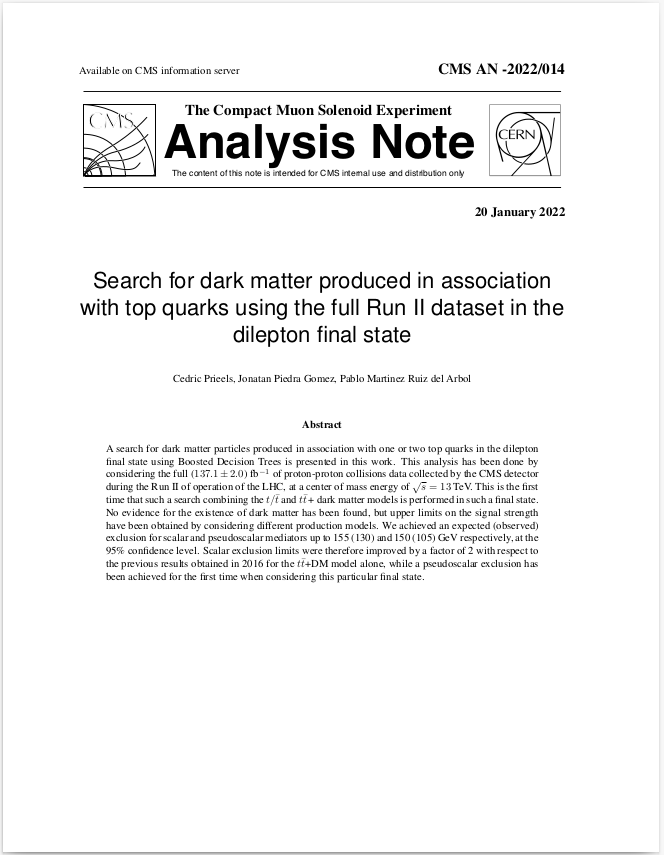
\includegraphics[width=1.0\textwidth]{figs/AN2.png}
	\end{column}
\end{columns}
\end{frame}

\begin{frame}{Focus of this thesis I}
\justifying
We are searching for \alert{dark matter produced in association with either one or two top quarks}. Several \textbf{simplified models} have been considered:

\begin{itemize} 
	\justifying
	\item Spin 1/2 DM $\chi$ ($\in [1, 55]$ GeV, Dirac fermion) \\
	\item Spin 0 scalar (S)/pseudoscalar (PS) mediator $\phi$/a (Yukawa-like structure of such interactions $\rightarrow$ \textbf{gain from the coupling of the mediator to top quarks}) \\
	\item Mediator mass $\in [10, 1000]$ GeV \\
	\item Coupling $g_{\chi}$ mediator/DM set to 1 (same for all $g_q$ couplings) \\
	%\item Most samples cross-section at NLO
	%\item No mixing between $\phi$ and the SM Higgs boson
\end{itemize}\vfill

\begin{center}
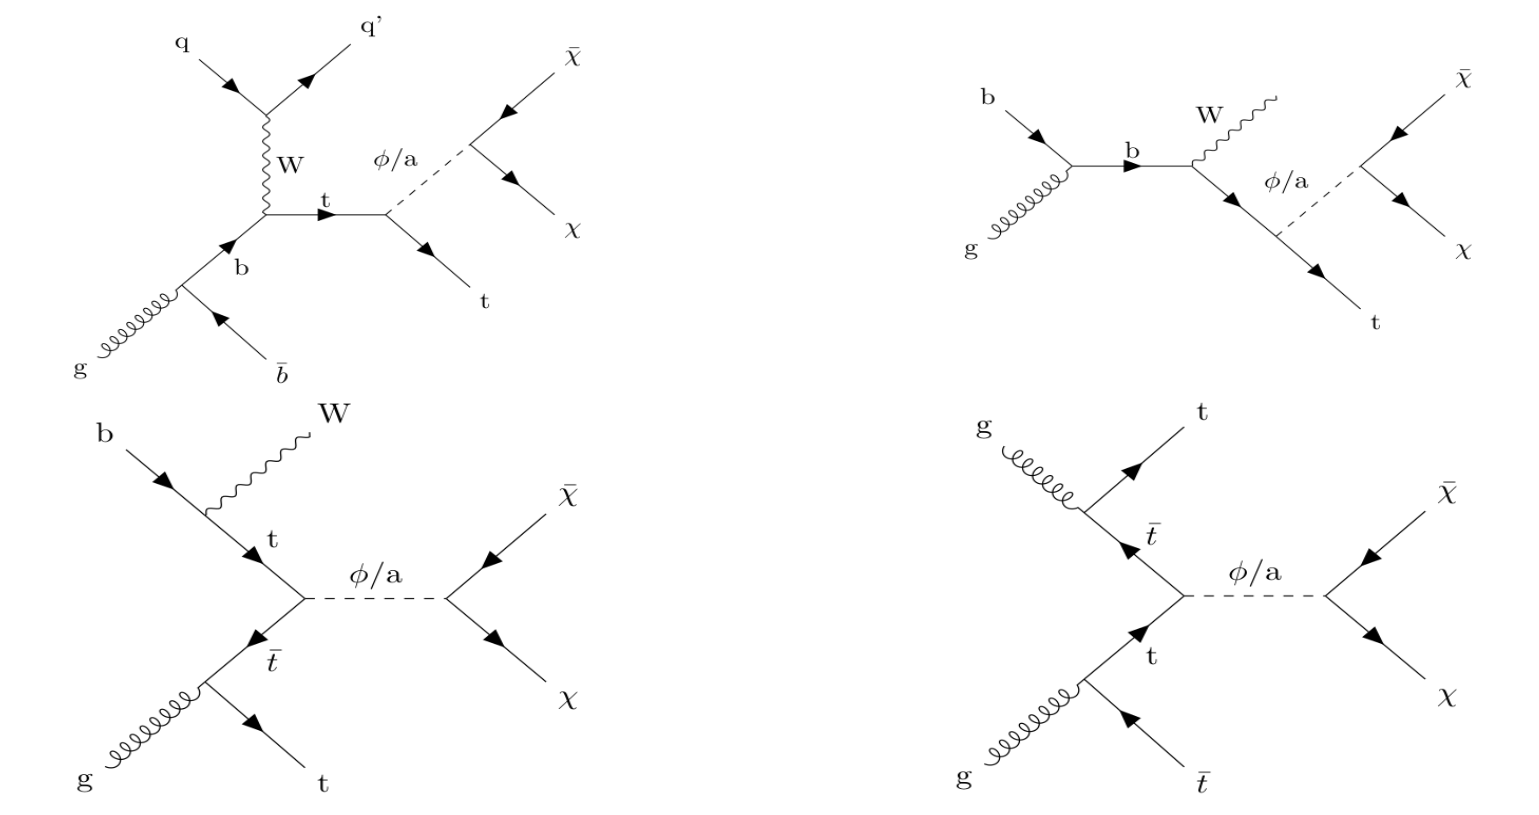
\includegraphics[width=0.78\textwidth, height=140pt]{figs/AllFeynman.png}
\end{center}

%\begin{columns}
%	\begin{column}{0.675\textwidth}
%		\begin{center}
%			\begin{block}{ \centering $t/ \bar t$+DM tW models}\end{block}	
%			%\alert{\textbf{$t$ + DM models}} \\ \vspace{5pt}
%			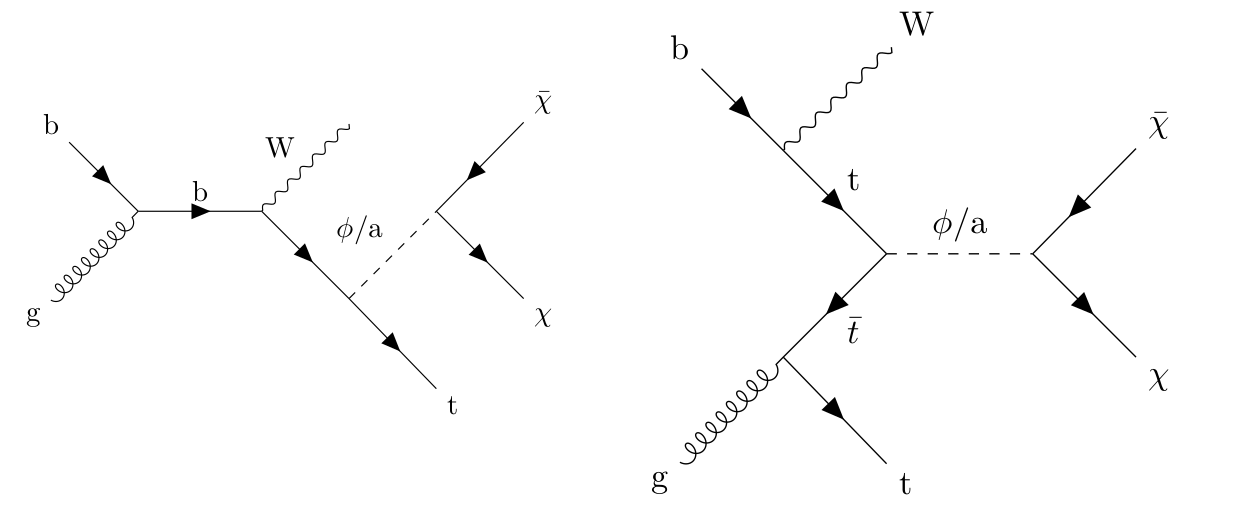
\includegraphics[width=1.0\textwidth]{figs/feynman_tDM_mine.png}
%    		 \end{center}
%	\end{column} \hfill
%	\begin{column}{0.3\textwidth}
%		\begin{center}
%			\begin{block}{\centering $t \bar t$+DM model}\end{block}				
%			%\alert{\textbf{$t \bar t$ + DM model}} \\ \vspace{5pt}
%			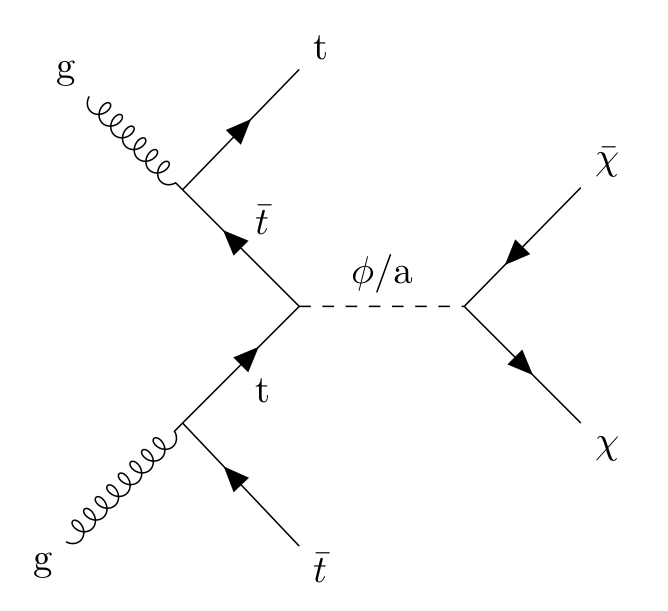
\includegraphics[width=1.0\textwidth]{figs/feynman_ttDM_mine.png}
%    		 \end{center}
%	\end{column} \hfill
%\end{columns} \vfill

%The Yukawa coupling typically favors searches for dark matter \textbf{produced in association with heavy quarks} such as this one. Such MET+X are heavily depend on the MET spectrum, which is expected to be larger for the signals than most backgrounds. \vfill
\end{frame}

\begin{frame}{Focus of this thesis II}
\justifying
The \textbf{typical final state} of such models is made out of:
\begin{itemize}
\justifying
\item 1 or 2 b-tagged jets coming from the decay of the top quark(s);
\item 2 W bosons, seen as a combination of jets and leptons depending on the channel;
\item Some ptmiss coming from the dark matter and the leptonic decay of the Ws;
\end{itemize} \vfill

In particular, we are studying the \alert{dilepton final state} in this work: 
\begin{itemize}
\justifying
\item Has the lowest branching ratio: BR($W \rightarrow l^+ + \nu_l) = (10.80 \pm 0.09)\%$ for each of the charged leptons (contains only $5\%$ of the signal events);
\item But, electrons and muons can usually be reconstructed better than jets, resulting in lower systematic uncertainties;
\item And this channel has the lowest number of backgrounds, with cross-sections typically lower, resulting in a better signal isolation.
\end{itemize} \vfill

%This channel is then \textbf{expected to be competitive with the hadronic and semi-leptonic channels}, especially when considering high mediator masses, which feature a higher global signal/background discrimination. \vfill
\end{frame}

\begin{frame}{Previous relevant results I}
\justifying
\vspace{5pt}
A similar analysis has already been carried out by CMS using 2016 data, considering only the $t \bar t$+DM signal and the dilepton final state (EXO-17-014). \vfill % \cite{PreviousDoubleTopAllLep13CMS}. \vfill

%\vspace{-10pt}
%\begin{figure}[htbp]
%\begin{center}
%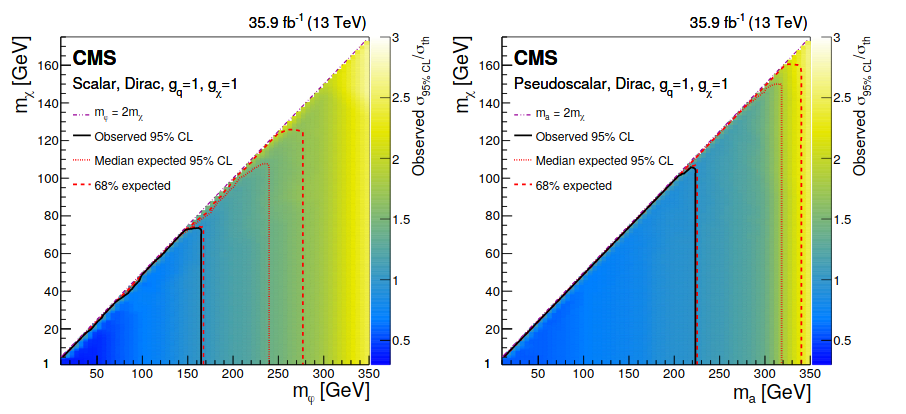
\includegraphics[width=11cm, height=4.8cm]{figs/CMSttbarExclusion.png}
%\end{center}
%\end{figure} \vfill

\begin{figure}[htbp]
\centering
\begin{minipage}[b]{.49\textwidth}
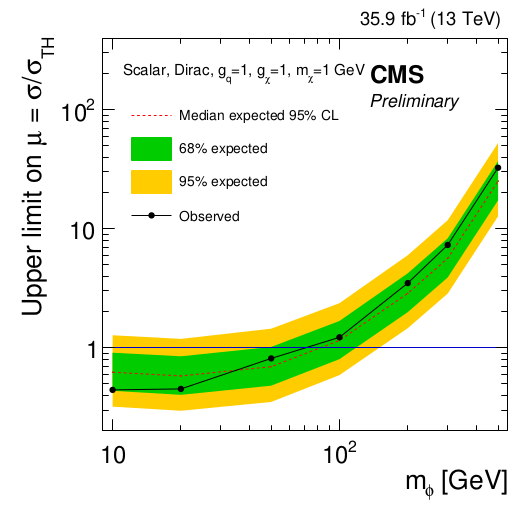
\includegraphics[width=5.4cm, height=4.7cm]{figs/Juan_S.png}
\end{minipage}\hfill
\begin{minipage}[b]{.49\textwidth}
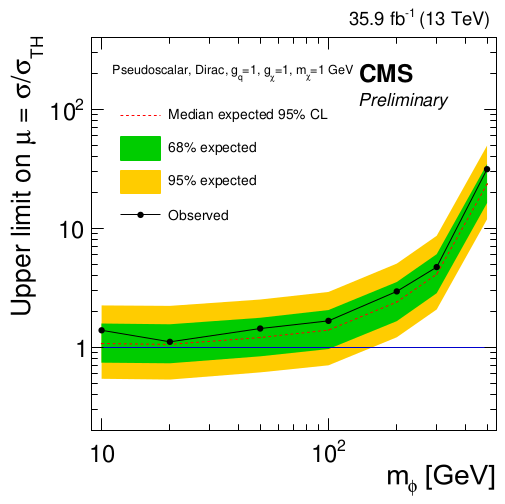
\includegraphics[width=5.4cm, height=4.7cm]{figs/Juan_PS.png}
\end{minipage}\hfill
\label{fig:Juan}
\end{figure}

This analysis \textbf{excluded scalar mediators} with masses below 80 GeV, while \textbf{no exclusion was achieved} when considering pseudoscalar mediators. \vfill
A combination of all the different final states was all also performed in EXO-16-049. \vfill

%The observed (expected) limits \textbf{excluded a pseudoscalar mediator} with mass below 220 (320) GeV, and \textbf{a scalar mediator} with mass below 160 (240) GeV. \vfill
%This provided the \alert{most stringent constraints} ever obtained at the time on the scalar dark matter mediator model. \vfill
\end{frame}

\begin{frame}{Previous relevant results II}
\justifying
\vspace{5pt}
A \textbf{combination} of both the $t/ \bar t$+DM and $t \bar t$+DM processes has also been performed (EXO-18-010). The inclusion of the single top signal process \alert{improved up to a factor 2} the limits obtained by the $t \bar t$ analysis on its own. This analysis: %\cite{PreviousSingleDoubleTopAllLep13CMS}. 

\begin{itemize}
\item Only considered the 2016 data-taking period;
\item And only considered the semi-leptonic and hadronic final states.
\end{itemize} \vfill

\begin{center}
\begin{columns}
	\begin{column}{1.0\textwidth}
		\begin{center}
			%\begin{block}{\centering $t \bar t$+DM limits}\end{block}				
			%\alert{\textbf{$t \bar t$ + DM model}} \\ \vspace{5pt}
			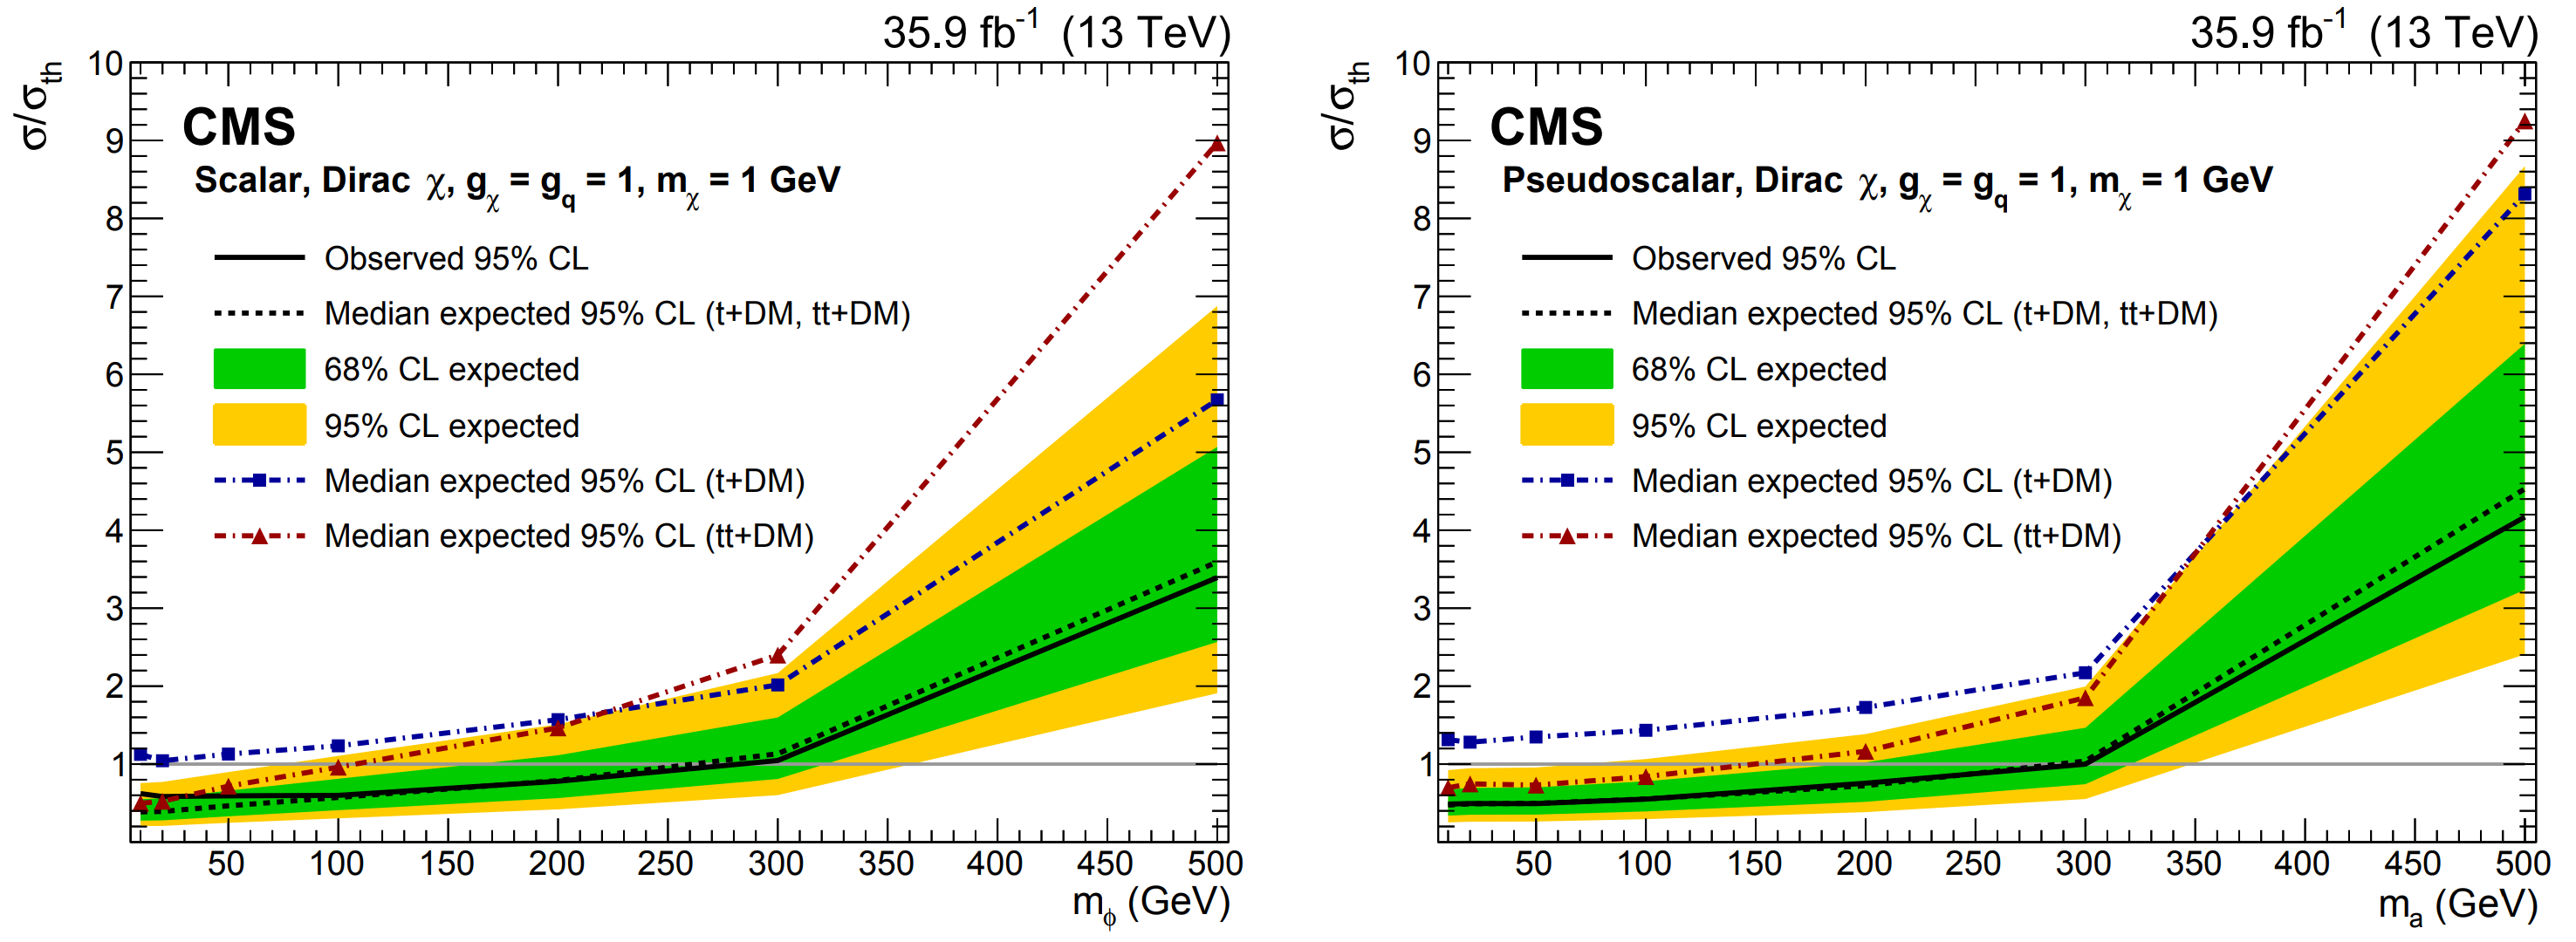
\includegraphics[width=1.0\textwidth]{figs/limitsprevious.png}
    		 \end{center}
	\end{column} \hfill
\end{columns}
\end{center} \vfill

Scalar (pseudoscalar) mediators were with this combination \textbf{excluded up to 290 (300) GeV} at the 95\% confidence level. \vfill %The inclusion of the full Run II dataset and the dilepton final state \textbf{is expected to improve these results}.
\end{frame}

\begin{frame}{Previous relevant results III}
\justifying
The ATLAS collaboration also obtained the exclusion limits obtained using the full Run II legacy dataset and considering the dilepton final state only (ATLAS-CONF-2020-046). \vfill

 \begin{figure}[htbp]
\centering
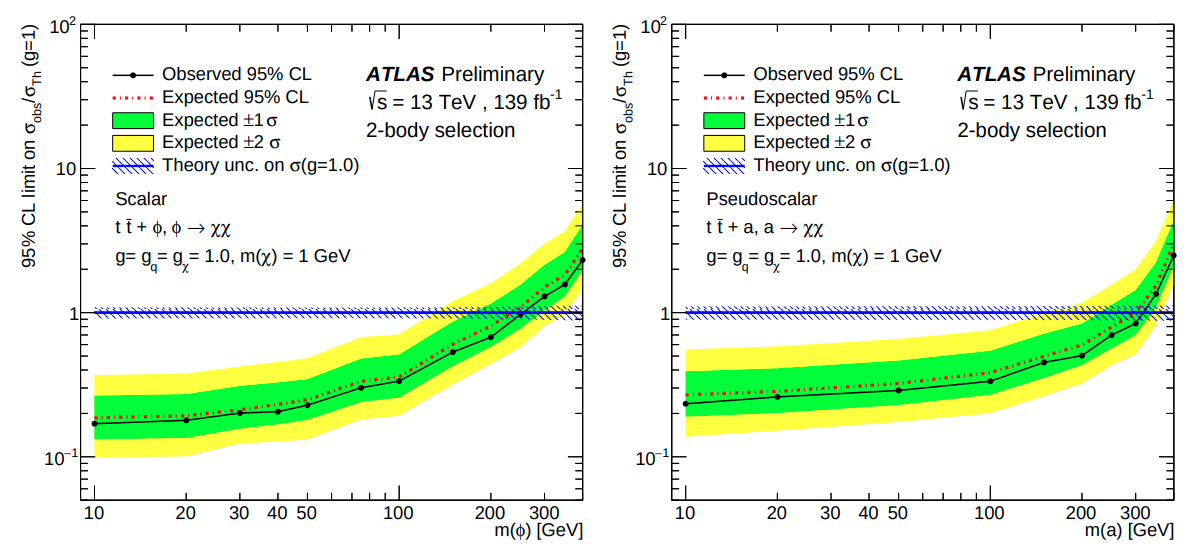
\includegraphics[width=10.5cm, height=4.7cm]{figs/ATLASICHEP.png}
\end{figure} \vfill

They obtained \textbf{expected scalar (pseudoscalar) exlusion limits of 250 (300) GeV}, even though  they used NLO cross-sections for the signals, around 30\% higher than ours. \vfill
\end{frame}












\begin{frame}[standout]
Analysis context
\end{frame}

\begin{frame}{Analysis strategy}
\justifying
Run II legacy paper being worked on, expected to \alert{combine both the $t/\bar t$+DM and $t \bar t$+DM searches}, and the 3 possible final states (hadronic, semi-leptonic and dileptonic). \\
\hspace{10pt} $\rightarrow$ Pre-approval process expected to start within a few weeks. \vfill

The effort is \textbf{globally common} between the groups (Wisconsin, DESY, IFCA) studying the different final states:
\begin{itemize}
\justifying
\item Objects are defined in a common way;
\item Control and signal region orthogonal between the channels.\\
$\rightarrow$ Number of leptons and b-jet categorization to improve the sensitivity by defining enriched $t/\bar t$+DM and $t \bar t$+DM regions.
\end{itemize} \vfill

This talk will however \textbf{be focused on the dilepton final state} only. \vfill
\begin{block}{}
\begin{center}
Given that my PhD thesis is now coming to an end, with no further extensions possible, I would like to ask the conveners to endorse the results presented next.
\end{center}
\end{block} \vfill
\end{frame}
















%\begin{frame}[standout]
%Hadronic final state \\
%Semi-leptonic final state
%\end{frame}
%
%\begin{frame}{Event selection}
%\justifying
%\begin{columns}
%		\hspace{5pt}
%		\begin{column}{0.64\textwidth}
%			\begin{center}
%				%\begin{block}{\centering Leading $p_T$}\end{block}	
%				%\alert{Leading $p_T$} \\ \vspace{5pt}
%     			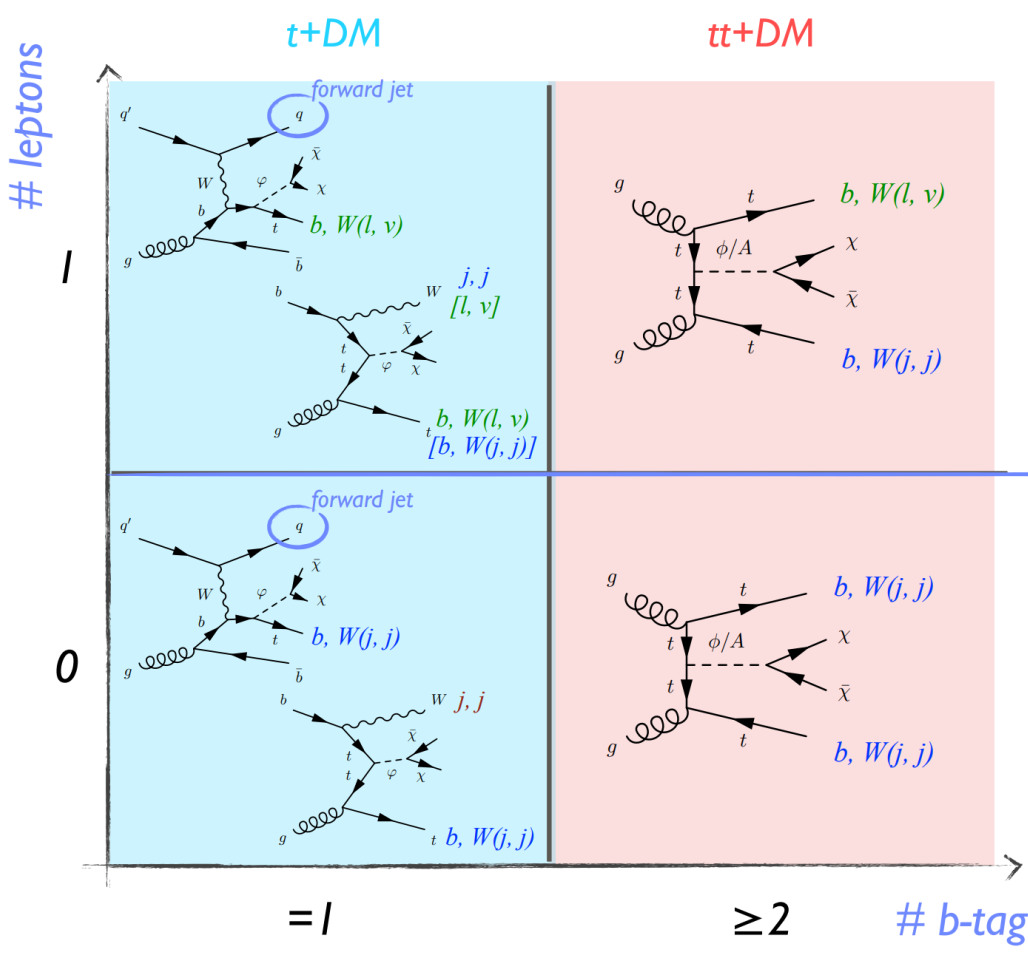
\includegraphics[width=\textwidth]{figs/semiHadronicSelection.png}
%    		\end{center}		
%		\end{column} \hfill
%		\begin{column}{0.39\textwidth}
%			\begin{center}
%				\begin{block}{\centering Single lepton}\end{block} \vfill
%				\begin{itemize}
%				\item Single lepton trigger
%				\item 1 isolated lepton (e, $\mu$)
%				\item $\geq 2$ jets
%				\item MET $> 160$ GeV
%				\item + $0, \geq 1$ forward jets ($|\eta|> 2.4$)
%				\end{itemize} \vfill
%				
%				\vspace{10pt}
%				\begin{block}{\centering All hadronic}\end{block} \vfill	
%				\begin{itemize}
%				\item MET trigger
%				\item Leptons veto (e, $\mu$)
%				\item $\geq 3$ jets
%				\item MET $> 250$ GeV
%				\item + $0, \geq 1$ forward jets
%				\end{itemize} \vfill
%    		\end{center}		
%		\end{column} \hfill
%\end{columns}
%\end{frame}





















\begin{frame}[standout]
Samples and objects
\end{frame}

\begin{frame}{Data and MC samples}
\justifying
\begin{block}{\centering Data}\end{block}
\alert{Single/double leptons datasets} built to avoid any eventual double counting, considering the 3 years of the Run II of operation of the LHC:
\begin{columns}
\hspace{15pt}
	\begin{column}{0.32\textwidth}
		\begin{itemize}
		\item ($35.9 \pm 0.9$) fb$^{-1}$
		\end{itemize}
	\end{column} \hfill
	\begin{column}{0.32\textwidth}
		\begin{itemize}
		\item ($41.5 \pm 1.0$)~fb$^{-1}$
		\end{itemize}
	\end{column} \hfill
	\begin{column}{0.32\textwidth}
		\begin{itemize}
		\item ($59.7 \pm 1.5$)~fb$^{-1}$
		\end{itemize}
	\end{column} \hfill
\end{columns} \vfill
\vspace{5pt}
A \textbf{blinding policy} has been followed at first, allowing us to only look at $1$~fb$^{-1}$ of data per year near the signal regions. \vfill
\vspace{10pt}
\begin{block}{\centering Backgrounds}\end{block}
The \alert{major backgrounds} have been considered from MC and read from NanoAOD. Each year has its corresponding MC samples:

\begin{itemize}
\justifying
\item $t \bar t$: decaying to both 1 and 2 leptons;%, TuneCUETP8M2 (2016) and TuneCP5 (2017, 2018);
\item Single top: s, t and tW channels considered;
\item Drell-Yan: HT-binned samples to increase the statistics, with a correction factor derived from data applied;
\item TTZ and TTW: usually grouped together as TTV, and considering both the hadronic and leptonic final states;
\item Others, such dibosons and tribosons production, all taken from MC directly.
\end{itemize} \vfill
\end{frame}

\begin{frame}{Signal samples}
\justifying
All the signals samples have been generated using MADGRAPH and PYTHIA8 (with the CP5 tune) at LO, while simulated events are then interfaced with a realistic model of the CMS detector using Geant4 [113] and are reconstructed using the official CMS reconstruction algorithms. \vfill
The $t/\bar t$+DM process was \textbf{produced privately} (central request has been made but not yet processed), while the $t \bar t$+DM was \textbf{generated centrally}. In both cases:

\begin{itemize}
\item Both scalar and pseudoscalar mediators are considered;
\item 400.000 events were produced for each mediator mass, from 10 to 1000 GeV;
\item The dark matter mass was set to 1 GeV, but additional samples ranging from 1 to 55 GeV were also produced;
\item All the $g_q$ and $g_\chi$ couplings were set to 1.
\end{itemize} \vfill

\textbf{Recommanded correction factors} (L1 ECAL prefiring in 2016 and 2017, HEM issue in 2018) are applied to the simulation. \vfill 
All the samples used and their cross-sections are listed in the backup. \vfill
\end{frame}

\begin{frame}{Signal samples}
\justifying
\begin{block}{\centering $t/\bar t$+DM}\end{block} \vspace{-10pt}
\begin{figure}[htbp]
\centering
\begin{minipage}[b]{.49\textwidth}
\vspace{-5pt}
\begin{block}{\centering Scalar}\end{block}
\begin{center}
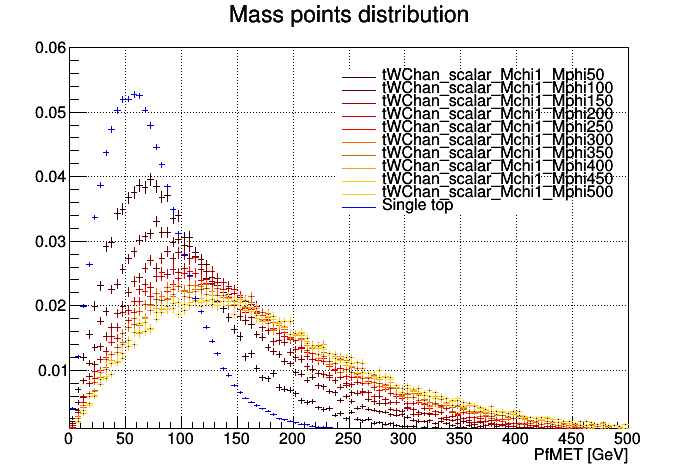
\includegraphics[width=5.2cm, height=3.5cm]{figs/singleTopScalarMETNorm.png}
\end{center}
\end{minipage}
\begin{minipage}[b]{.02\textwidth}\end{minipage}
\begin{minipage}[b]{.49\textwidth}
\vspace{-5pt}
\begin{block}{\centering Pseudoscalar}\end{block}
\begin{center}
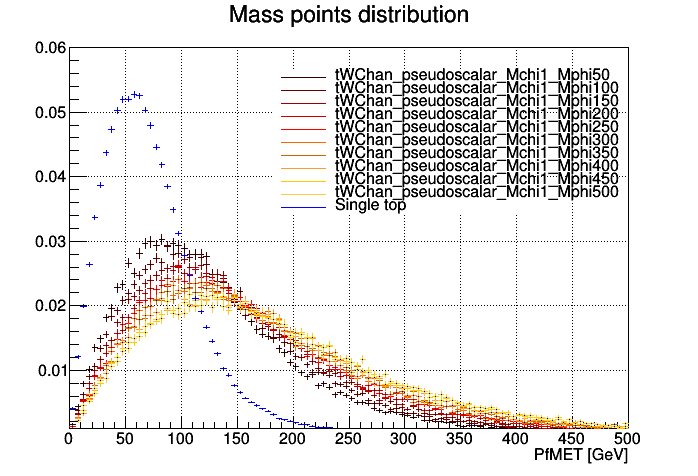
\includegraphics[width=5.2cm, height=3.5cm]{figs/singleTopPseudoMETNorm.png}
\end{center}
\end{minipage}
\end{figure} \vfill

\vspace{-5pt}
\begin{block}{\centering $t \bar t$+DM}\end{block} \vspace{-10pt}
\begin{figure}[htbp]
\centering
\begin{minipage}[b]{.49\textwidth}
\begin{center}
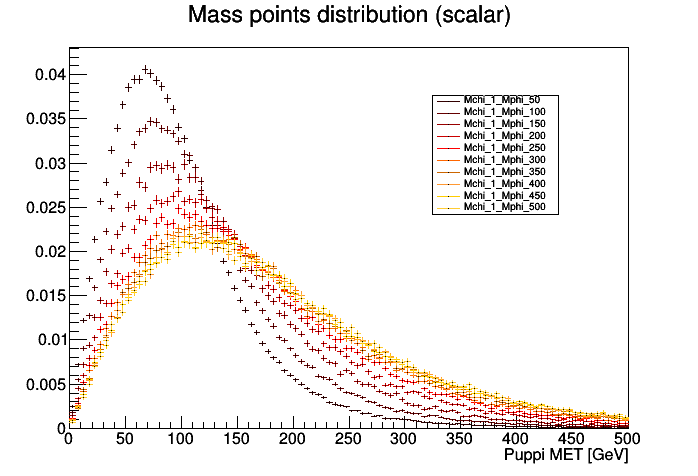
\includegraphics[width=5.2cm, height=3.5cm]{figs/scalarMETmChi1Norm.png}
\end{center}
\end{minipage}\hfill
\begin{minipage}[b]{.49\textwidth}
\begin{center}
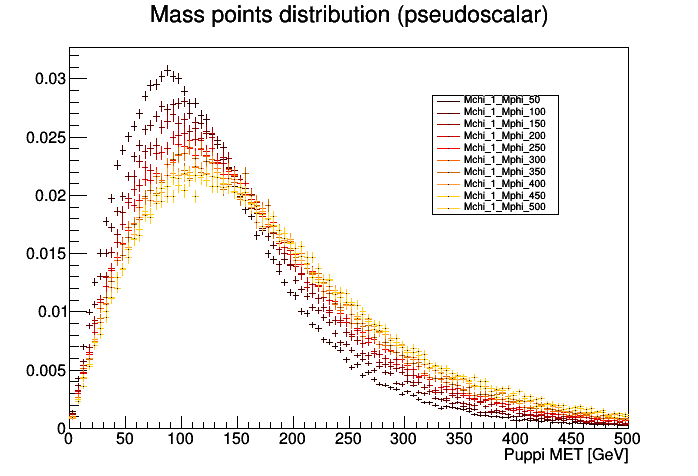
\includegraphics[width=5.2cm, height=3.5cm]{figs/pseudoscalarMETmChi1Norm.png}
\end{center}
\end{minipage} \hfill
\end{figure} \vfill
\end{frame}

\begin{frame}{Objects definition I}
\justifying
%We are currently using the following objects: \vfill

\vspace{5pt} \begin{block}{\centering Triggers}\end{block} \vspace{-6pt}
\begin{itemize}
\justifying
\item \alert{Single and double lepton triggers} combined to gain statistics, and any possible double counting of events in multiple trigger is taken care of;
\item Trigger and lepton $p_T$ carefully chosen to avoid any turn-on effect;
\item SingleMuon, SingleEle, DoubleMuon, DoubleEG, MuonEG (2016) and SingleMuon, EGamma, DoubleMuon, MuonEG (2017/2018) data streams considered;
\item All the triggers used and their efficiencies (computed using orthogonal MET datasets) are listed in the backup.
\end{itemize} \vfill

\begin{block}{\centering Leptons}\end{block} \vspace{-6pt}
\begin{itemize}
\justifying
\item Analysis relies on the selection of events with two leptons, with a leading (trailing) $p_T >$ 25 (20) GeV and $|\eta| < 2.4$;
\item \alert{Medium cut based} POG WP used for electrons without additional ISO cut;
\item \alert{Medium cut based} POG WP for muons with tight ISO (pfRelIso04\_all $< 0.15$);
\item Additional small cuts on the impact parameters to reduce the non-prompt contamination in the ptmiss tail ($|d_0| < 0.05$ cm, $|d_z| < 0.1$ cm, $S_{3D}^d < 4$).
\end{itemize}
\end{frame}

\begin{frame}{Objects definition II}
\justifying
\vspace{5pt} \begin{block}{\centering Jets}\end{block}
\begin{itemize}
\justifying
\item Clustered from the PF candidates using the \textbf{anti-kT algorithm};
\item Basic selection: $p_T > 30$ GeV, $|\eta| < 2.4$;
\item \alert{Tight JET/MET POG} working point (efficiency and background rejection $>$ 98\%), tight jet PU ID applied to jets with $p_T < 50$ GeV to reject PU jets contamination;
\item $\Delta R > 0.4$ away from any lepton passing the criteria established for analysis to prevent signal leptons clustered as jets from entering the jet counting.
\end{itemize} \vfill

\vspace{5pt}
\begin{block}{\centering B-tag}\end{block}
\begin{itemize}
\justifying
\item B-Tagging and Vertexing POG \alert{deep CSV b-tag medium working point} (high efficiency, misidentification rate for a light jet as a b-jet $\sim 1\%$).
%\item B-tagging weight larger than 0.6321, 0.4941 or 0.4184 (2016, 2017 or 2018).
\end{itemize} \vfill

\vspace{5pt}
\begin{block}{\centering Missing transverse momentum}\end{block}
\begin{itemize}
\justifying
\item \alert{PfType1MET} considered by propagating the JECs to the ptmiss;
\item All recommended \textbf{filters applied} to filter anomalous high ptmiss events due to several detector issues, such as eventual dead cells in the calorimeters;
\item XY-shift ($\phi$ modulation fix) and EE noise (2017) corrections applied on top.
\end{itemize} \vfill
\end{frame}



































\begin{frame}[standout]
Event selection
\end{frame}

\begin{frame}{Event selection}
\justifying
\vspace{5pt}
\begin{block}{\centering Minimal event selection}\end{block} \vfill
\vspace{-5pt}

We require for the analysis:
\begin{itemize}
\item Two opposite sign leptons, with leading (trailing) $p_T >$ 25 (20) GeV;
\item Third lepton veto ($p_T < 10$ GeV);
\item $m_{ll} > 20$ GeV to avoid low mass resonances;
\item At least 1 jet.
\end{itemize} \vfill

\vspace{5pt}
\begin{block}{\centering Pre-selection region}\end{block} \vfill
\vspace{-5pt}

A pre-selection region is then defined by additionally asking for:
\begin{itemize}
\item At least 1 medium deep CSV b-jet (misidentification rate of light jets around 1\%);
\item A 76-106 GeV Z-veto on the $ee$ and $\mu \mu$ channels;
\item ptmiss $>$ 100 GeV and $M_{T2}^{ll} >$ 80 GeV to keep this region orthogonal to the $t \bar t$ control regions used by the semi-leptonic channel.
\end{itemize} \vfill

This region is used as the basis for the definition of our signals regions. \vfill
\end{frame}

\begin{frame}{Minimal event selection region}
\begin{columns}
%\begin{column}{1.09\textwidth}
%\begin{block}{\centering $ll$ channel}\end{block}
%\end{column}
\end{columns} \vspace{-5pt}
\begin{columns}
		\begin{column}{0.33\textwidth}
			\begin{center}
			\vspace{-8pt}
			\begin{block}{\centering 2016}\end{block}\vspace{10pt}
     			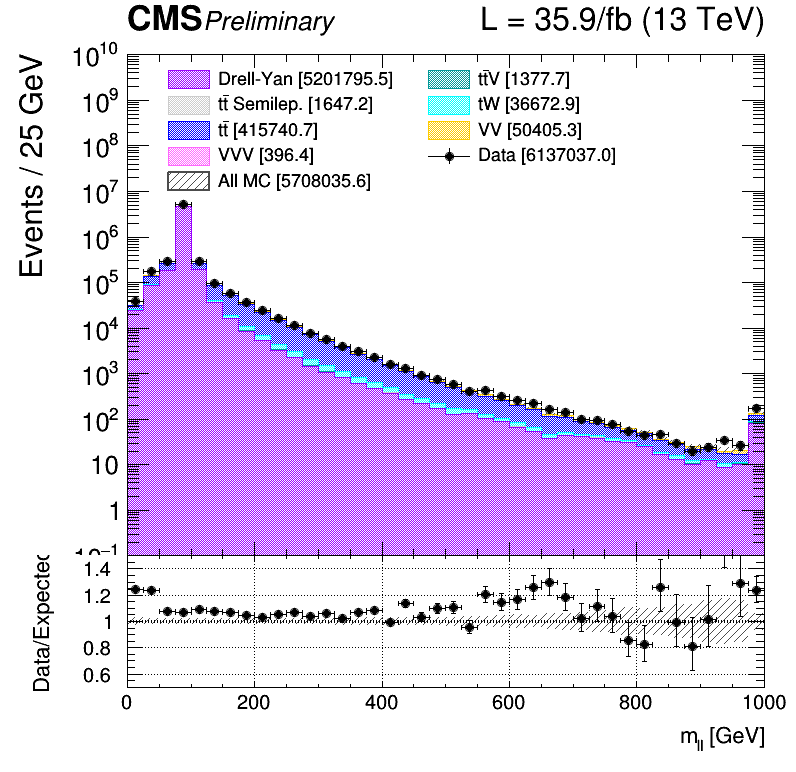
\includegraphics[width=1.0\textwidth, height=100pt]{figs/2016/log_cratio_inclusiveCR_ll_mll.png}
    		\end{center}		
		\end{column} 
		\begin{column}{0.33\textwidth}
			\begin{center}
			\vspace{-8pt}
			\begin{block}{\centering 2017}\end{block}\vspace{10pt}
     			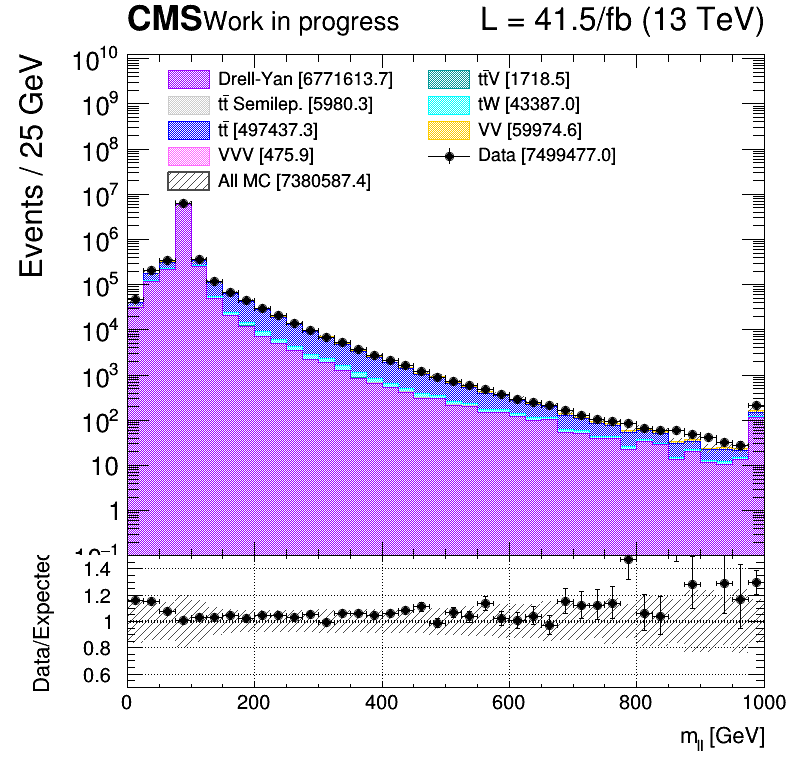
\includegraphics[width=1.0\textwidth, height=100pt]{figs/2017/log_cratio_inclusiveCR_ll_mll.png}
    		\end{center}		
		\end{column} 
		\begin{column}{0.33\textwidth}
			\begin{center}
			\vspace{-8pt}
			\begin{block}{\centering 2018}\end{block}\vspace{10pt}
     			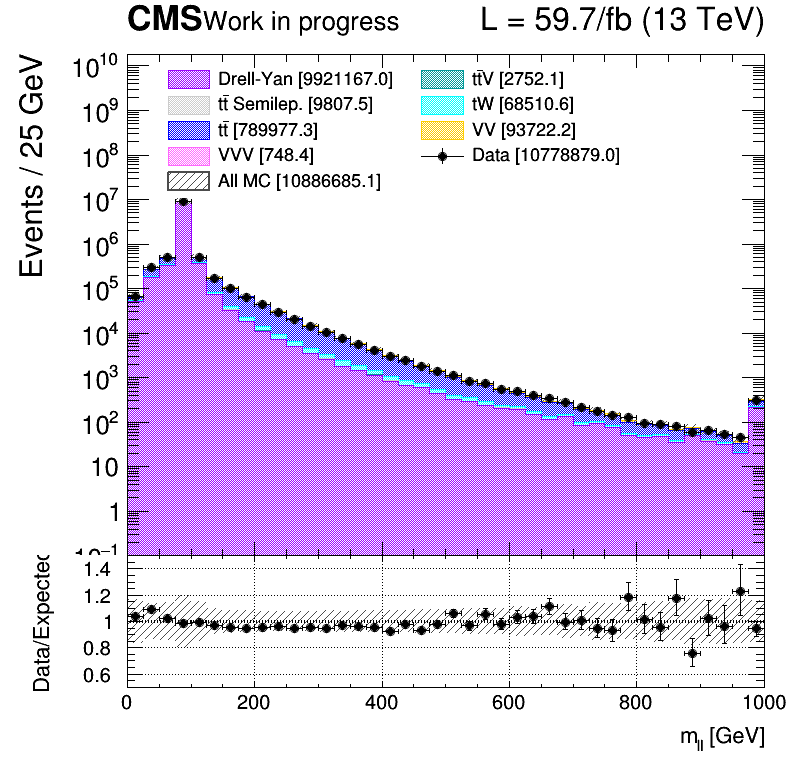
\includegraphics[width=1.0\textwidth, height=100pt]{figs/2018/log_cratio_inclusiveCR_ll_mll.png}
    		\end{center}		
		\end{column}
\end{columns}
\vspace{-5pt}
\begin{columns}
		\begin{column}{0.33\textwidth}
			\begin{center}
				%\begin{block}{\centering Puppi MET}\end{block}	
     			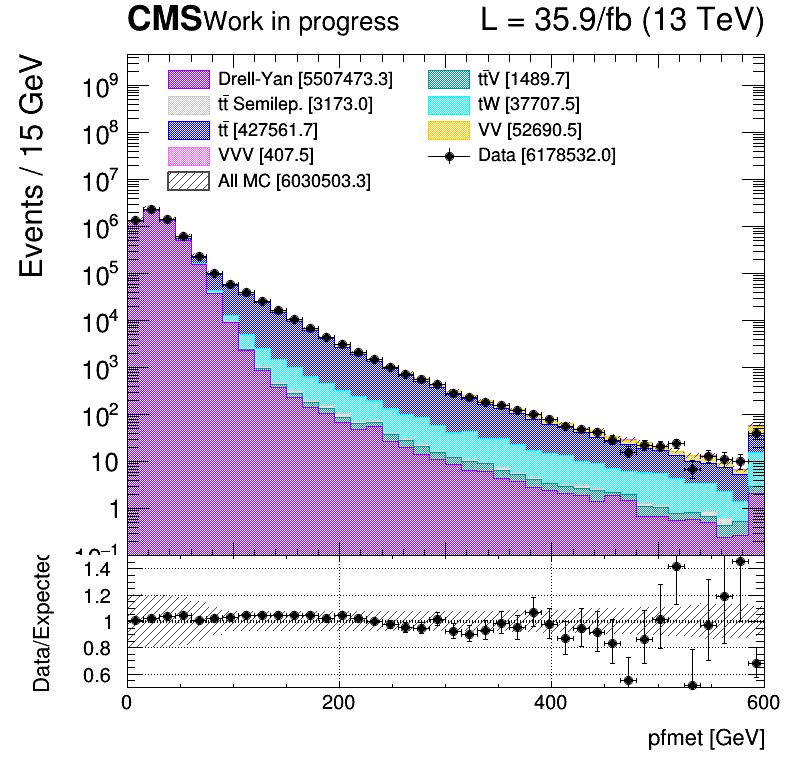
\includegraphics[width=1.0\textwidth, height=100pt]{figs/2016/log_cratio_inclusiveCR_ll_METcorrected_pt.png}
    		\end{center}		
		\end{column}
		\begin{column}{0.33\textwidth}
			\begin{center}
				%\begin{block}{\centering njet}\end{block}	
     			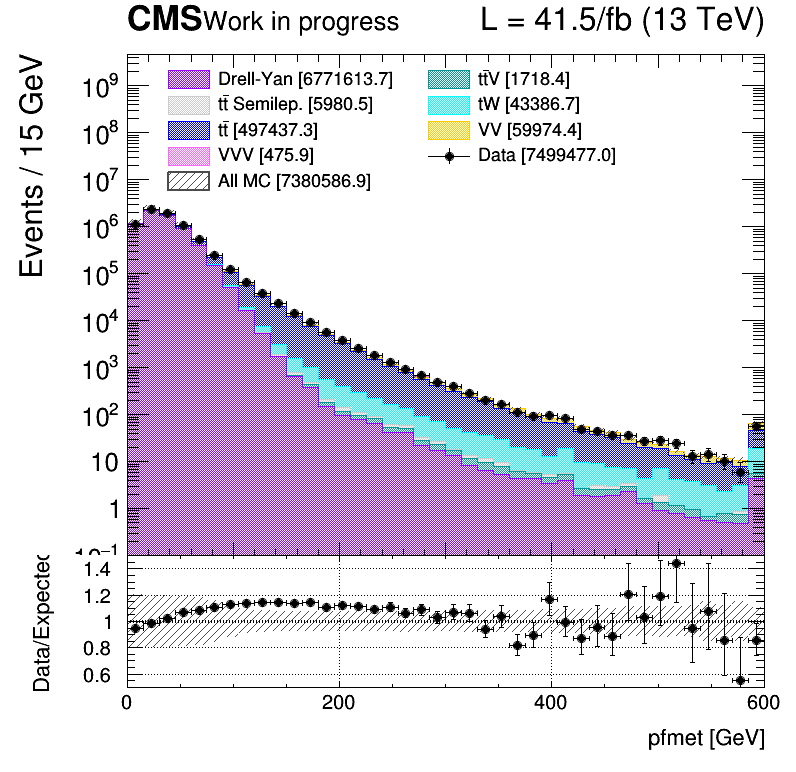
\includegraphics[width=1.0\textwidth, height=100pt]{figs/2017/log_cratio_inclusiveCR_ll_METcorrected_pt.png}
    		\end{center}		
		\end{column}
		\begin{column}{0.33\textwidth}
			\begin{center}
				%\begin{block}{\centering nbjet}\end{block}	
     			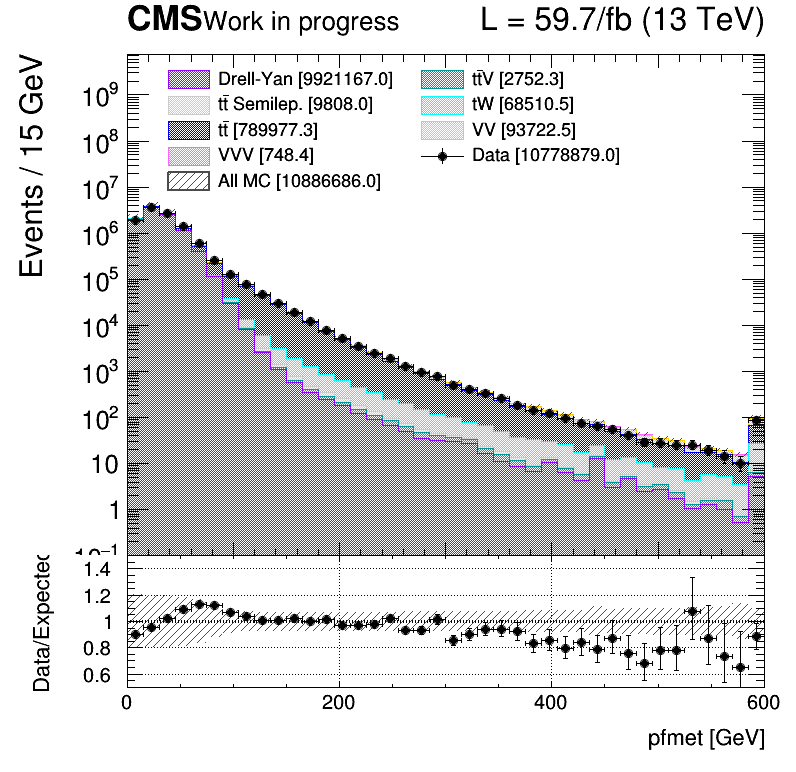
\includegraphics[width=1.0\textwidth, height=100pt]{figs/2018/log_cratio_inclusiveCR_ll_METcorrected_pt.png}
    		\end{center}		
		\end{column}
\end{columns} \vfill
\end{frame}

\begin{frame}{Pre-selection region}
\begin{columns}
%\begin{column}{1.09\textwidth}
%\begin{block}{\centering $ll$ channel}\end{block}
%\end{column}
\end{columns} \vspace{-5pt}
\begin{columns}
		\begin{column}{0.33\textwidth}
			\begin{center}
			\vspace{-8pt}
			\begin{block}{\centering 2016}\end{block}\vspace{10pt}
     			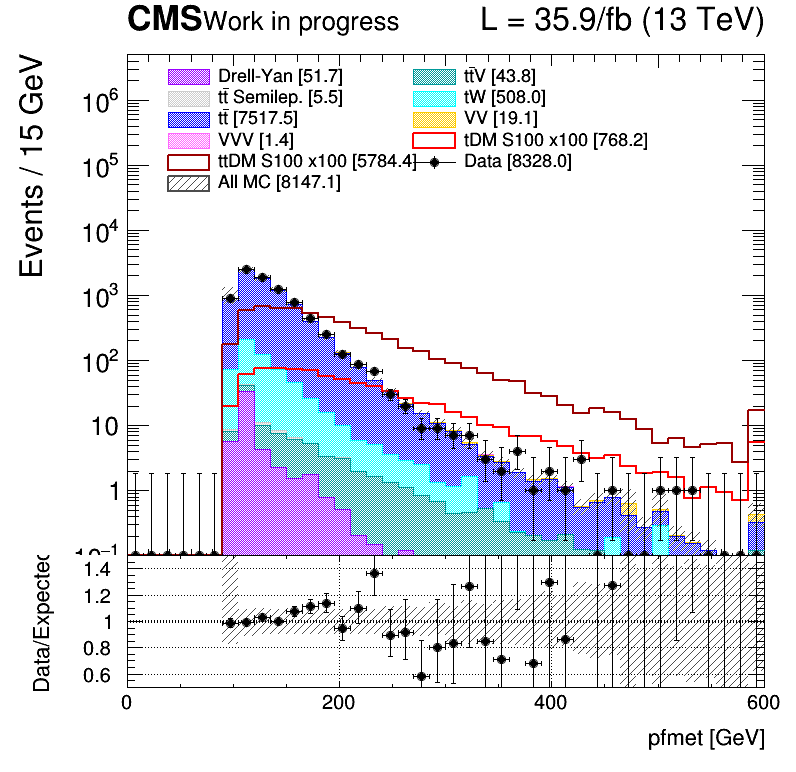
\includegraphics[width=1.0\textwidth, height=100pt]{figs/2016/SmearSR-ttDM-scalar100/log_cratio_topCR_ll_METcorrected_pt.png}
    		\end{center}		
		\end{column} 
		\begin{column}{0.33\textwidth}
			\begin{center}
			\vspace{-8pt}
			\begin{block}{\centering 2017}\end{block}\vspace{10pt}
     			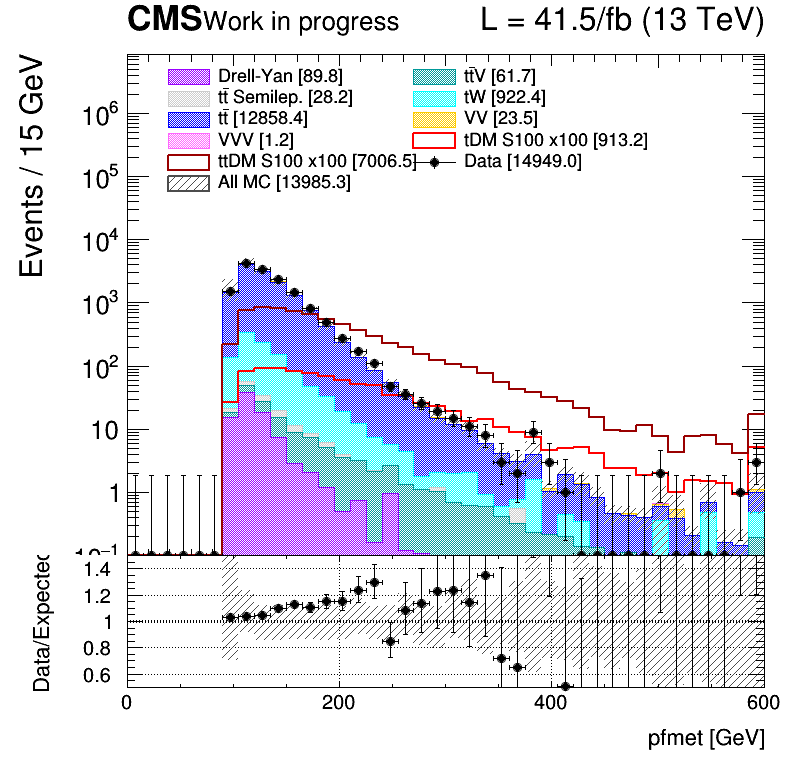
\includegraphics[width=1.0\textwidth, height=100pt]{figs/2017/SmearSR-ttDM-scalar100/log_cratio_topCR_ll_METcorrected_pt.png}
    		\end{center}		
		\end{column} 
		\begin{column}{0.33\textwidth}
			\begin{center}
			\vspace{-8pt}
			\begin{block}{\centering 2018}\end{block}\vspace{10pt}
     			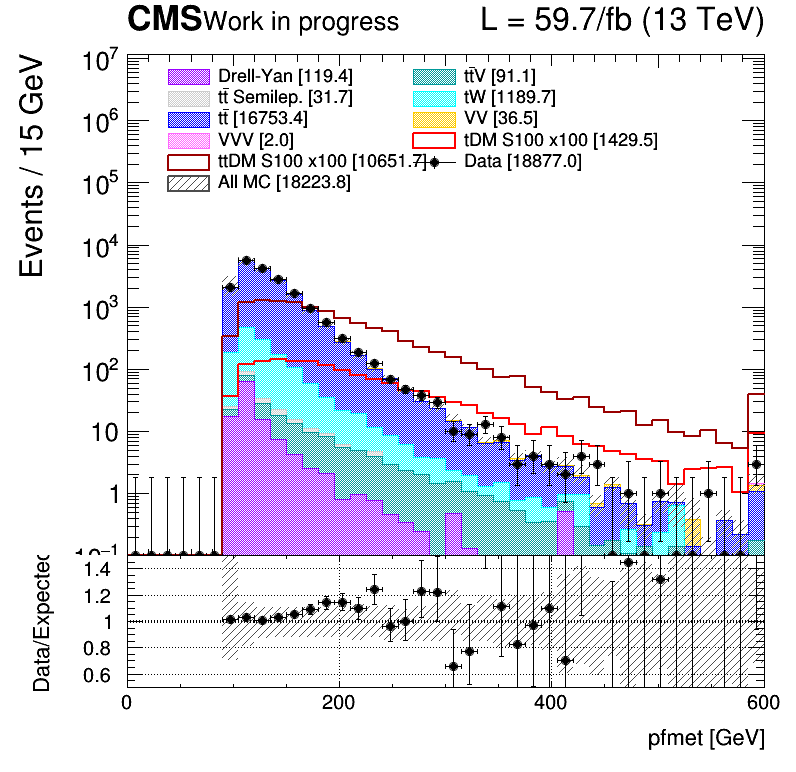
\includegraphics[width=1.0\textwidth, height=100pt]{figs/2018/SmearSR-ttDM-scalar100/log_cratio_topCR_ll_METcorrected_pt.png}
    		\end{center}		
		\end{column}
\end{columns}
\vspace{-5pt}
\begin{columns}
		\begin{column}{0.33\textwidth}
			\begin{center}
				%\begin{block}{\centering Puppi MET}\end{block}	
     			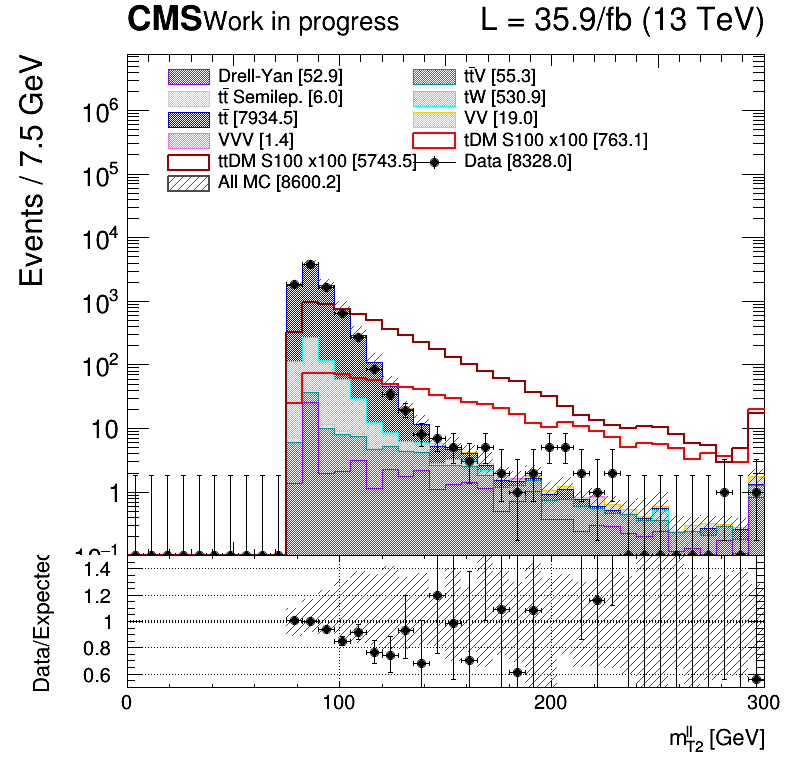
\includegraphics[width=1.0\textwidth, height=100pt]{figs/2016/SmearSR-ttDM-scalar100/log_cratio_topCR_ll_mt2ll.png}
    		\end{center}		
		\end{column}
		\begin{column}{0.33\textwidth}
			\begin{center}
				%\begin{block}{\centering njet}\end{block}	
     			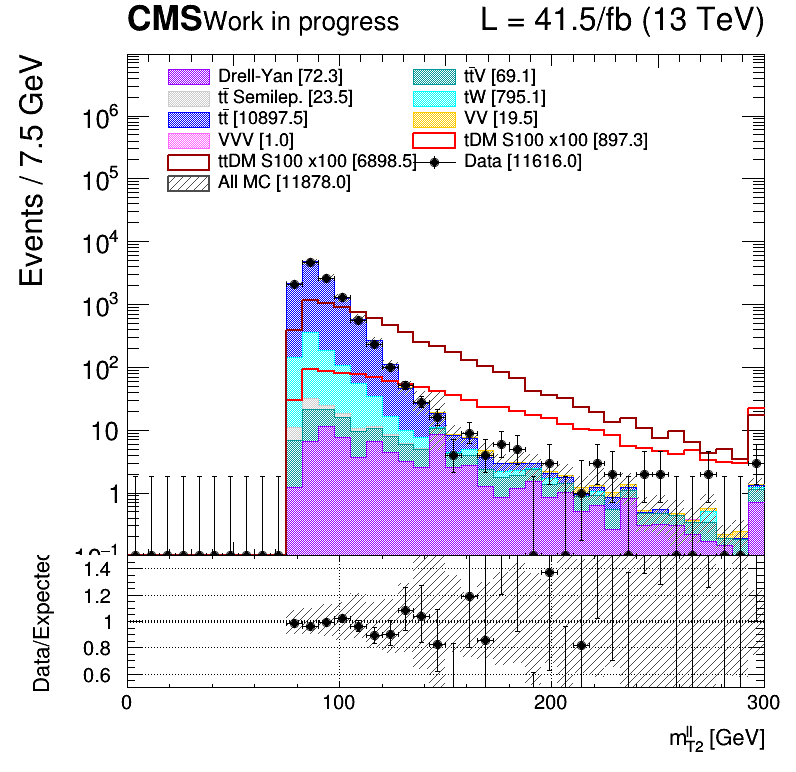
\includegraphics[width=1.0\textwidth, height=100pt]{figs/2017/SmearSR-ttDM-scalar100/log_cratio_topCR_ll_mt2ll.png}
    		\end{center}		
		\end{column}
		\begin{column}{0.33\textwidth}
			\begin{center}
				%\begin{block}{\centering nbjet}\end{block}	
     			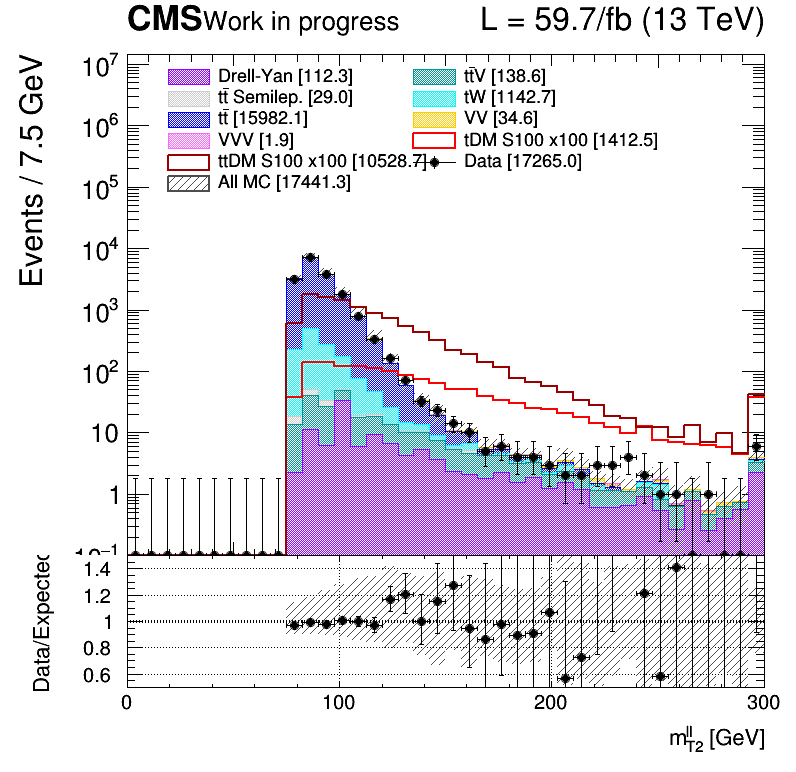
\includegraphics[width=1.0\textwidth, height=100pt]{figs/2018/SmearSR-ttDM-scalar100/log_cratio_topCR_ll_mt2ll.png}
    		\end{center}		
		\end{column}
\end{columns} \vfill
\end{frame}









\begin{frame}[standout]
Background prediction methods
\end{frame}

\begin{frame}{Main background processes}
\justifying
The backgrounds are predicted either directly from \alert{Monte-Carlo simulations or from semi data-driven methods}.

\begin{itemize}
\justifying
\item The \textbf{$t \bar t$ and the single top} are taken from simulation accounting for all the variations in the generation parameters. Several parameters (QCD scale, PDF variation,...) are varied and included as a systematic (see later);
\item The \textbf{Drell-Yan} yields are obtained from a semi data-driven method using the excluded same flavor region on the Z peak as control region;
\item \textbf{ttV, diboson, triboson processes and other minor backgrounds} are taken directly from MC simulations.
\end{itemize} \vfill

\textbf{Recommanded correction factors} (L1 ECAL prefiring in 2016 and 2017, HEM issue in 2018) are also applied to the simulation. \vfill 

\textbf{Data validation regions} enriched in top and Drell-Yan have been explored to ensure the quality of the prediction made.\vfill
\end{frame}

\begin{frame}{Top control region}
\justifying
Same as the pre-selection region but with ptmiss $> 50$ GeV and $60 < M_{T2}^{ll} < 80$ GeV. \vfill

\begin{columns}
		\begin{column}{0.33\textwidth}
			\begin{center}
			\vspace{-8pt}
			\begin{block}{\centering 2016}\end{block}\vspace{5pt}
     			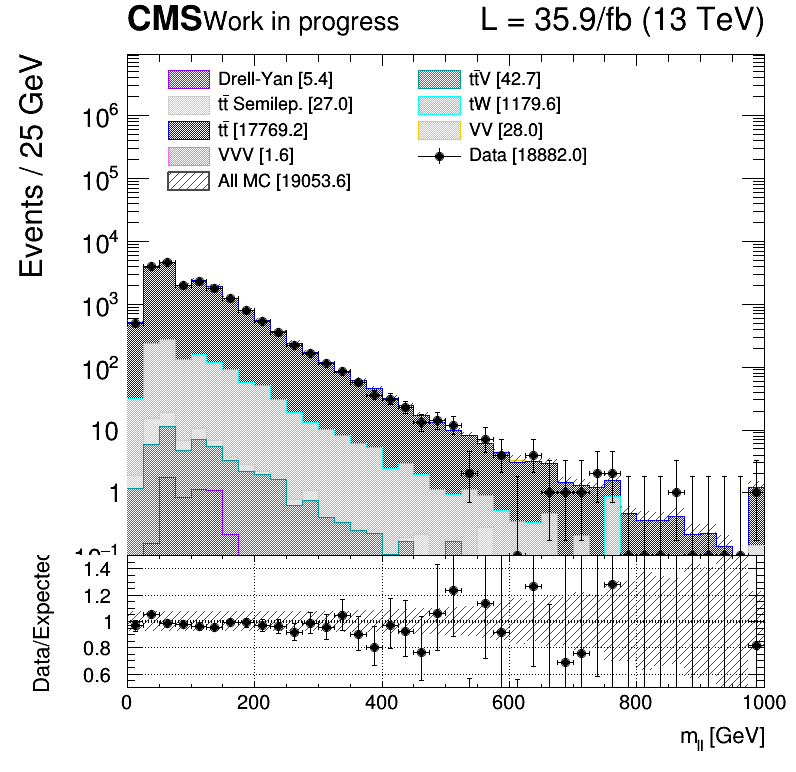
\includegraphics[width=1.0\textwidth, height=95pt]{figs/2016/log_cratio_ttbarCR_ll_mll.png}
    		\end{center}		
		\end{column} 
		\begin{column}{0.33\textwidth}
			\begin{center}
			\vspace{-8pt}
			\begin{block}{\centering 2017}\end{block}\vspace{5pt}
     			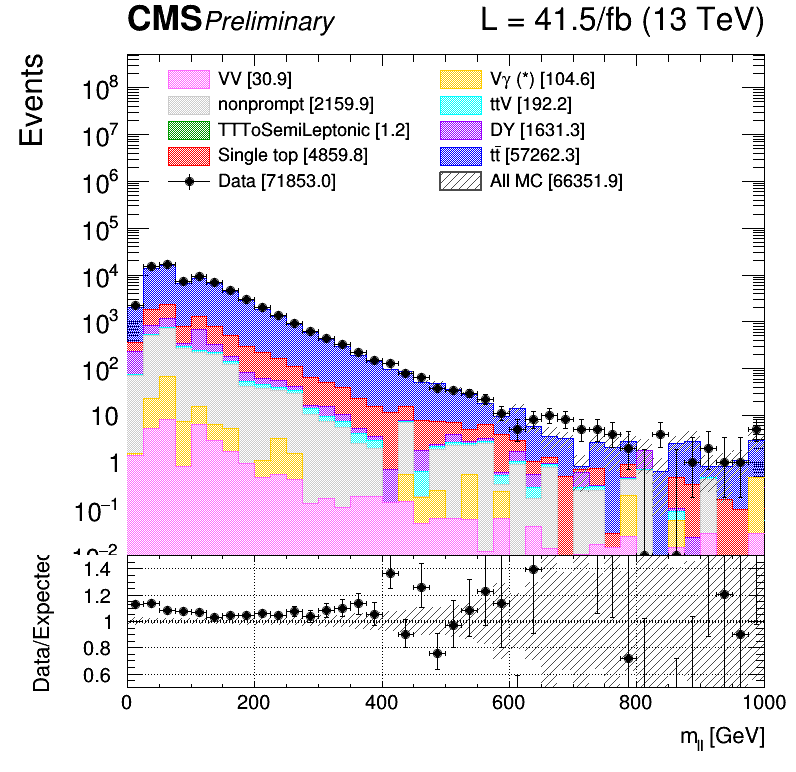
\includegraphics[width=1.0\textwidth, height=95pt]{figs/2017/log_cratio_ttbarCR_ll_mll.png}
    		\end{center}		
		\end{column} 
		\begin{column}{0.33\textwidth}
			\begin{center}
			\vspace{-8pt}
			\begin{block}{\centering 2018}\end{block}\vspace{5pt}
     			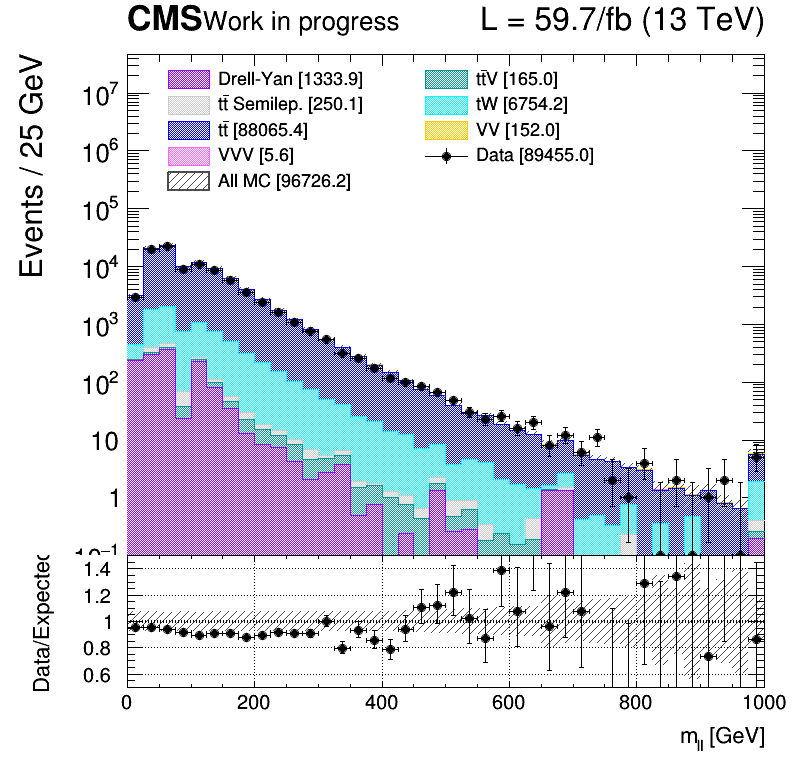
\includegraphics[width=1.0\textwidth, height=95pt]{figs/2018/log_cratio_ttbarCR_ll_mll.png}
    		\end{center}		
		\end{column}
\end{columns}

\vspace{-5pt}
\begin{columns}
		\begin{column}{0.33\textwidth}
			\begin{center}
				%\begin{block}{\centering Puppi MET}\end{block}	
     			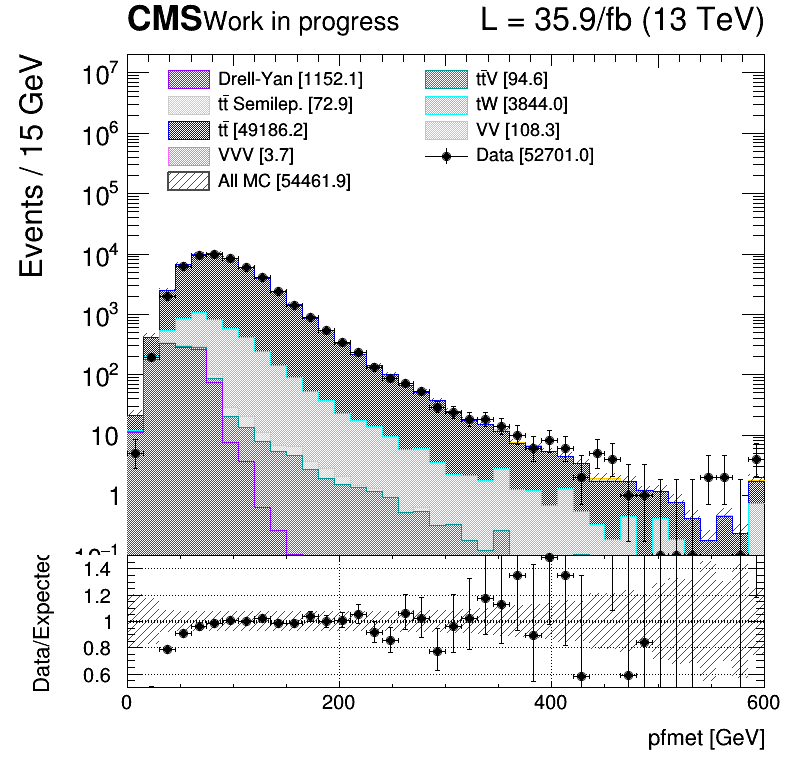
\includegraphics[width=1.0\textwidth, height=95pt]{figs/2016/log_cratio_ttbarCR_ll_METcorrected_pt.png}
    		\end{center}		
		\end{column}
		\begin{column}{0.33\textwidth}
			\begin{center}
				%\begin{block}{\centering njet}\end{block}	
     			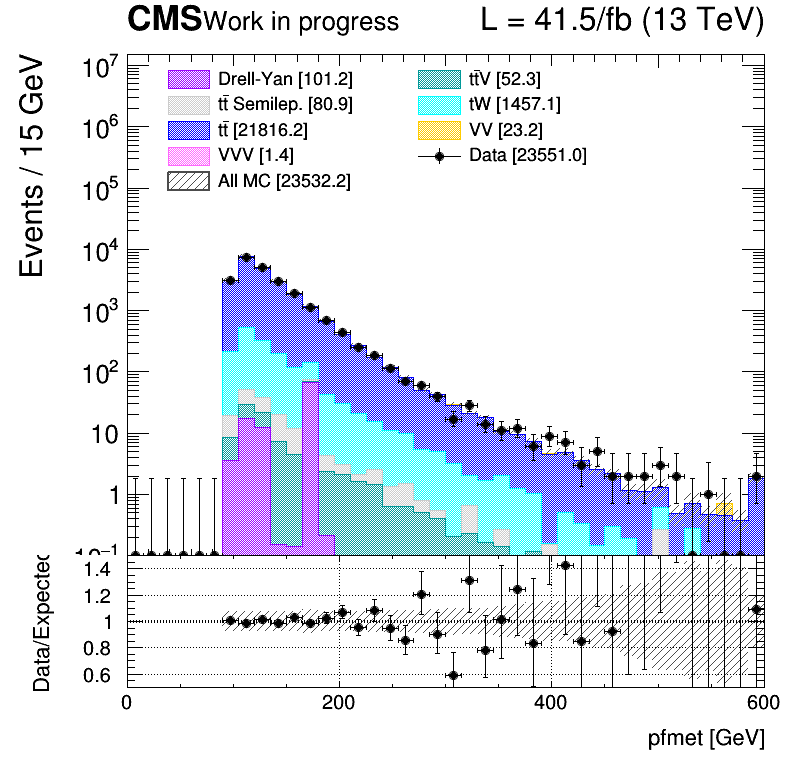
\includegraphics[width=1.0\textwidth, height=95pt]{figs/2017/log_cratio_ttbarCR_ll_METcorrected_pt.png}
    		\end{center}		
		\end{column}
		\begin{column}{0.33\textwidth}
			\begin{center}
				%\begin{block}{\centering nbjet}\end{block}	
     			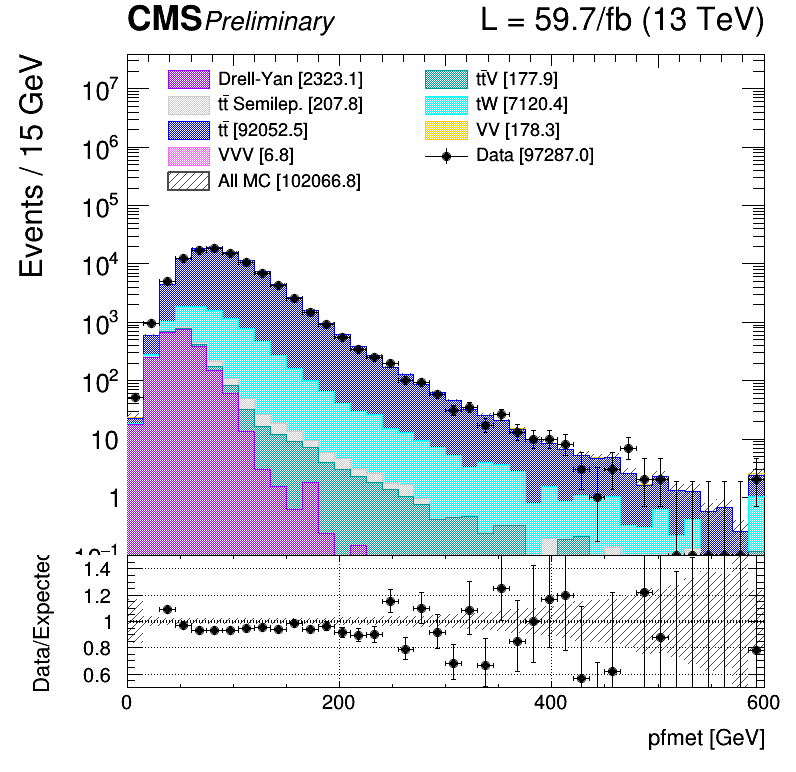
\includegraphics[width=1.0\textwidth, height=95pt]{figs/2018/log_cratio_ttbarCR_ll_METcorrected_pt.png}
    		\end{center}		
		\end{column}
\end{columns} \vfill
\end{frame}

\begin{frame}{DY Rin-out method}
\justifying
We want to \textbf{estimate the DY yields outside of the Z-peak from the data} in the minimal event selection region:

\begin{itemize}
\justifying
\item Given the presence of large backgrounds (such as $t \bar t$) in the analysis region, we go inside of the Z-peak to compute the \alert{Rin-out factor}:
\begin{equation*}
N^{out}_{DY} = N^{in}_{DY, data} \cdot \kappa \cdot \left (\frac{N^{out}_{DY, MC}}{N^{in}_{DY, MC}} \right ) \equiv N^{in}_{DY, data} \cdot \frac{R_{out/in,\text{ } MC}^{0bj}}{R_{out/in,\text{ } data}^{0bj}} \cdot R_{out/in,\text{ } MC}
\end{equation*}
\item To avoid any bias, the contamination of non-peaking backgrounds is removed and we correct this factor by the ratio $\kappa$ between the data/MC transfer factors in a CR close to the SR (asking for 0 b-jet instead of 1);
\item We then get this Rin-out in \textbf{bins of ptmiss and for each channel ($ee$, $\mu \mu$)}:
\end{itemize}

\begin{figure}[htbp]
\begin{center}
\begin{minipage}[b]{.32\textwidth}
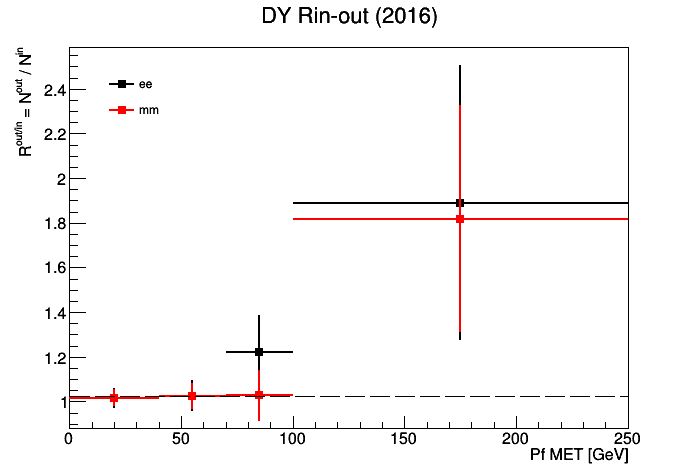
\includegraphics[width=4cm, height=3cm]{figs/Rinout2016_data.png}
\end{minipage} \hfill
\begin{minipage}[b]{.32\textwidth}
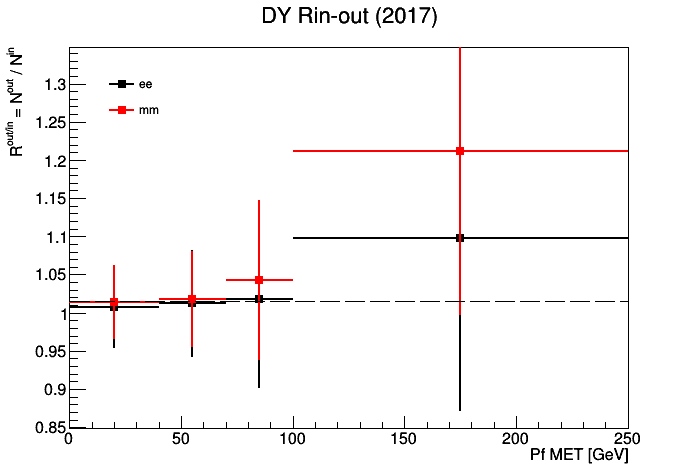
\includegraphics[width=4cm, height=3cm]{figs/Rinout2017_data.png}
\end{minipage} \hfill
\begin{minipage}[b]{.32\textwidth}
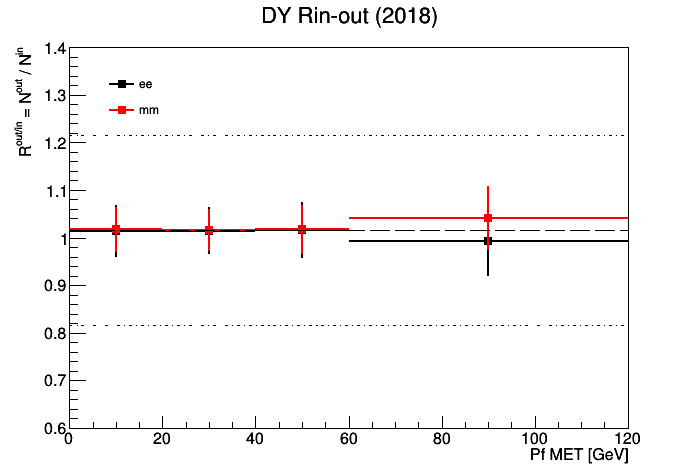
\includegraphics[width=4cm, height=3cm]{figs/Rinout2018_data.png}
\end{minipage} \hfill
\end{center}
\end{figure} \vfill

\vspace{-5pt}
A flat scale factor and a fixed 20\% systematic uncertainty is then applied to the DY. \vfill
\end{frame}

\begin{frame}{DY control region}
\justifying
Same as the pre-selection region but with ptmiss $>$ 30 GeV and Z-veto reversed.
\begin{columns}
		\begin{column}{0.33\textwidth}
			\begin{center}
			\vspace{-8pt}
			\begin{block}{\centering 2016}\end{block}\vspace{5pt}
     			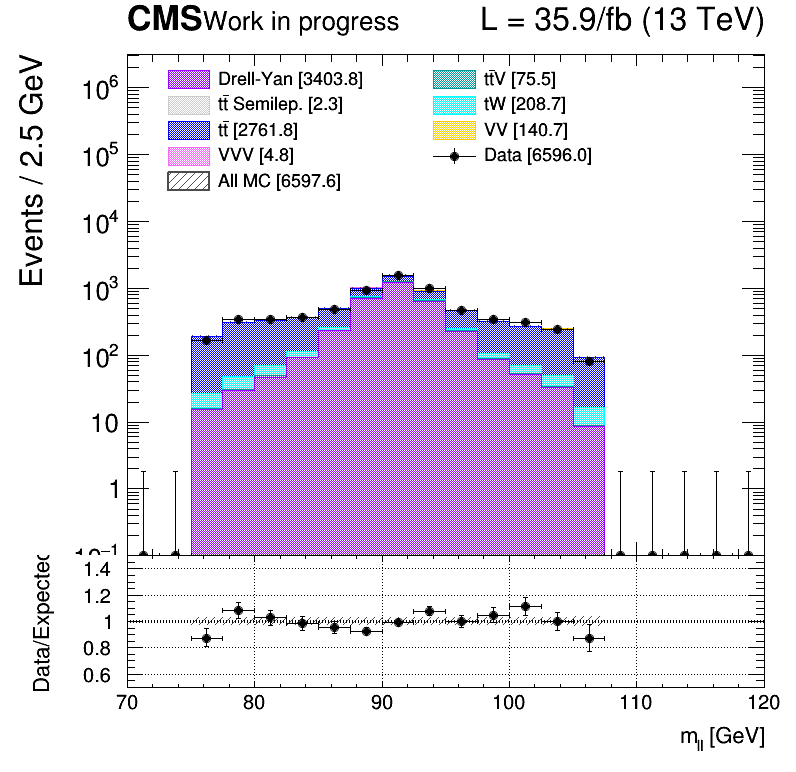
\includegraphics[width=1.0\textwidth, height=95pt]{figs/2016/log_cratio_dyCR_ll_mllpeak.png}
    		\end{center}		
		\end{column} 
		\begin{column}{0.33\textwidth}
			\begin{center}
			\vspace{-8pt}
			\begin{block}{\centering 2017}\end{block}\vspace{5pt}
     			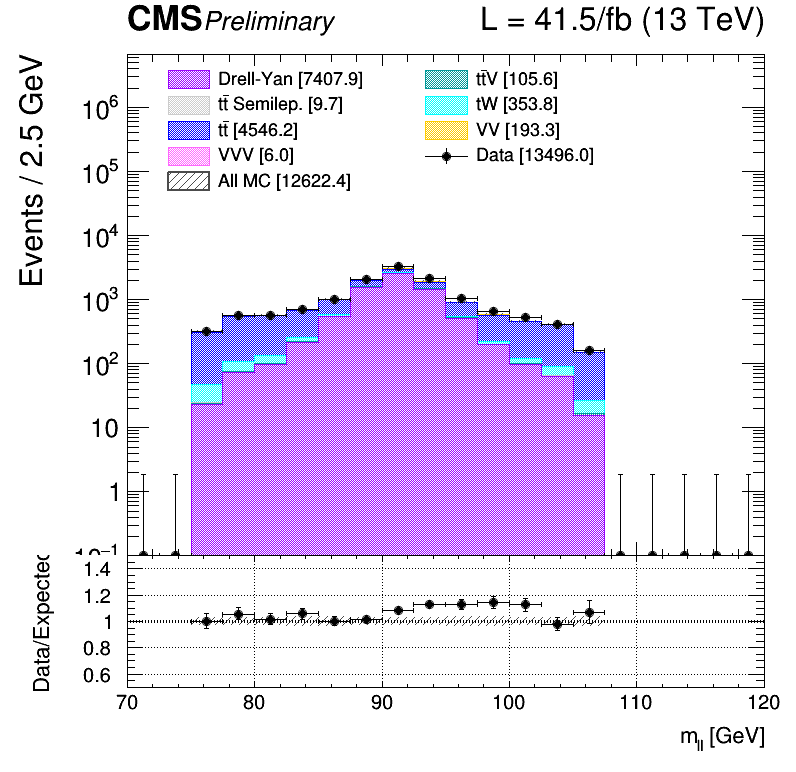
\includegraphics[width=1.0\textwidth, height=95pt]{figs/2017/log_cratio_dyCR_ll_mllpeak.png}
    		\end{center}		
		\end{column} 
		\begin{column}{0.33\textwidth}
			\begin{center}
			\vspace{-8pt}
			\begin{block}{\centering 2018}\end{block}\vspace{5pt}
     			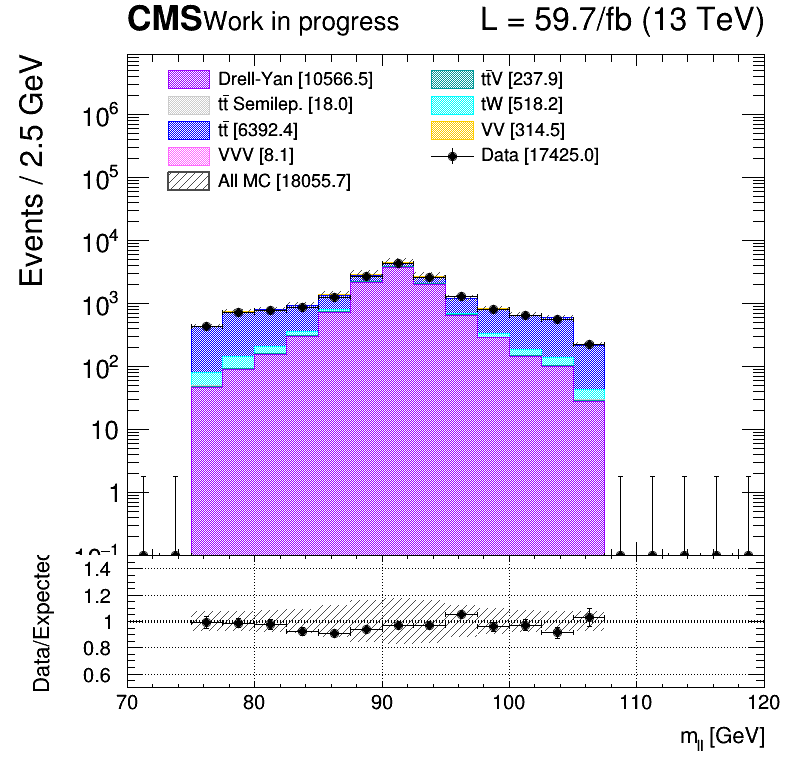
\includegraphics[width=1.0\textwidth, height=95pt]{figs/2018/log_cratio_dyCR_ll_mllpeak.png}
    		\end{center}		
		\end{column}
\end{columns}
\vspace{-5pt}
\begin{columns}
		\begin{column}{0.33\textwidth}
			\begin{center}
				%\begin{block}{\centering Puppi MET}\end{block}	
     			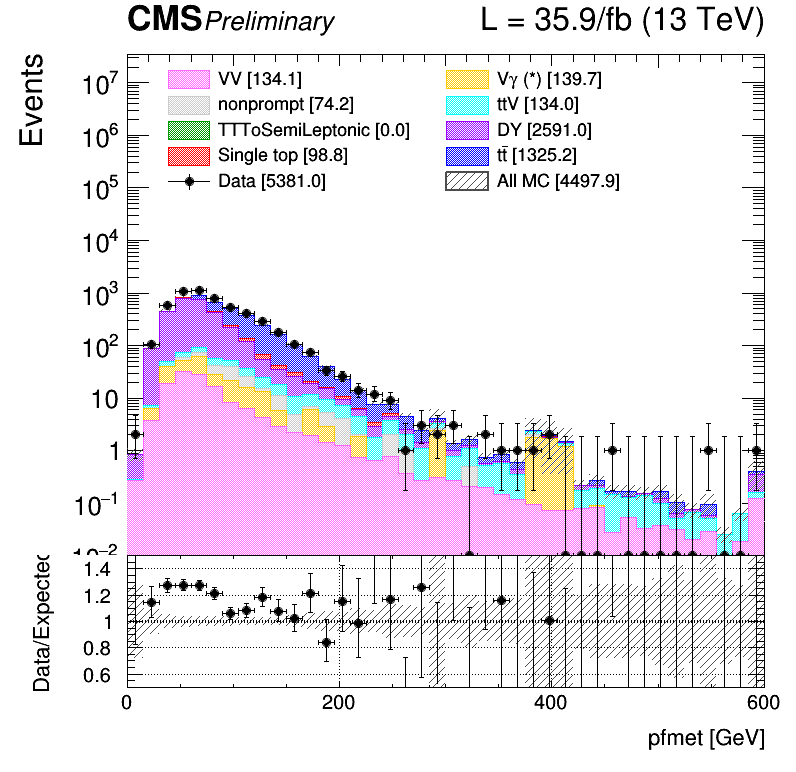
\includegraphics[width=1.0\textwidth, height=95pt]{figs/2016/log_cratio_dyCR_ll_METcorrected_pt.png}
    		\end{center}		
		\end{column}
		\begin{column}{0.33\textwidth}
			\begin{center}
				%\begin{block}{\centering njet}\end{block}	
     			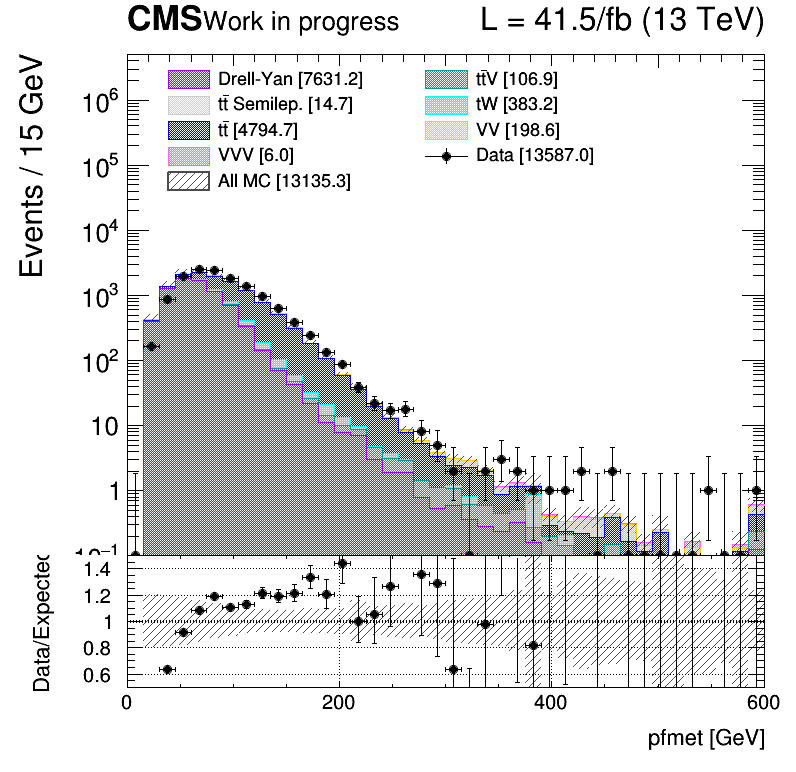
\includegraphics[width=1.0\textwidth, height=95pt]{figs/2017/log_cratio_dyCR_ll_METcorrected_pt.png}
    		\end{center}		
		\end{column}
		\begin{column}{0.33\textwidth}
			\begin{center}
				%\begin{block}{\centering nbjet}\end{block}	
     			\includegraphics[width=1.0\textwidth, height=95pt]{figs/2018/log_cratio_dyCR_ll_METcorrected_pt.png}
    		\end{center}		
		\end{column}
\end{columns} \vfill

%The 0-bjet correction allows us to fix the data/MC discrepancies observed. A large systematic uncertainty is associated to this background, minor in the signal regions. \vfill
\end{frame}












\begin{frame}[standout]
Signal extraction
\end{frame}

\begin{frame}{Global strategy}
\justifying
In this analysis, \alert{two different signal regions} are being used, targeting each one of our signals of interest, each based on the pre-selection region:
\begin{itemize}
\item One targeting the $t/\bar t$+DM signal, by considering events having exactly 1 jet, or exactly 2 jets and 1 b-jet;
\item Another one targeting the $t \bar t$+DM signal, by considering events having exactly 2 jets and more than 1 b-jet, or more than 2 jets.
\end{itemize} \vfill

Several different \alert{discriminating variables} (ptmiss, stranverse mass $M_{T2}^{ll}$, spin correlated variables, etc.) are being considered. \vfill

Many of such variables require knowledge of the top quark and anti-quark 4-momenta, only available after a \textbf{complete reconstruction of the $t \bar t$ system}, performed whenever possible (details in the backup). \vfill

A BDT combines the discriminating power of all the variables considered, and a ANN is being used as a cross check. A complete optimization was followed in order to select features which maximize the performance. \vfill
\end{frame}

\begin{frame}{Discriminating variables I}
\justifying
Several discriminating variables (all detailed in the backup) are considered, such as:
\begin{itemize}
\item The stransverse mass $M_{T2}^{ll}$
\item The missing transverse momentum 
\item The number of b-jets (only in the $t \bar t$+DM signal region) and $m_{bl}^t$ variable, useful to separate our two signals
\item Several spin correlated variables
\item $r_{2l}$ and $r_{2l4j}$, defined as the ratio between the ptmiss and the $p_T$ of the leptons (+ the 4 first jets for $r_{2l4j}$)
\item The dark $p_T$ and overlapping factor naturally arising from the top reconstruction
\item Other variables, such as the angle $\Delta \phi$ between the ptmiss and the two leptons, and total transverse mass massT.
\end{itemize} \vfill

\begin{table}
\begin{center}
\resizebox{0.6\textwidth}{!}{
\begin{tabular}{ c|c|c|c|c } 
 \hline
 & \multicolumn{2}{c}{\textbf{$t/\bar t$+DM region}} & \multicolumn{2}{c}{\textbf{$t \bar t$+DM region}} \\
 Rank & Variable & Importance & Variable & Importance \\
 \hline
 1 & $M_{T2}^{ll}$ & $5.96 \cdot 10^{-1}$ & $M_{T2}^{ll}$ & $5.87 \cdot 10^{-1}$ \\
 2 & $E_{T}^{\text{miss}}$ & $5.32 \cdot 10^{-1}$ & $E_{T}^{\text{miss}}$ & $5.09 \cdot 10^{-1}$ \\
 3 & massT & $3.11 \cdot 10^{-1}$ & massT & $3.98 \cdot 10^{-1}$ \\ 
 4 & $r2l4j$ & $1.70 \cdot 10^{-1}$ & $r2l4j$ & $3.45 \cdot 10^{-1}$ \\ 
 5 & $m_{bl}^t$ & $7.05 \cdot 10^{-2}$ & $m_{bl}^t$ & $1.72 \cdot 10^{-1}$ \\
 6 & $r2l$ & $2.63 \cdot 10^{-2}$ & Dark $p_T$ & $3.92 \cdot 10^{-2}$ \\
\hline
\end{tabular}
}
\end{center}
\end{table} \vfill	
\end{frame}


\begin{frame}{Discriminating variables II}
\begin{columns}
\begin{column}{1.09\textwidth}
\begin{block}{\centering 2016}\end{block} \vspace{5pt}
\end{column}
\end{columns} \vspace{-5pt}
\begin{columns}
		\begin{column}{0.33\textwidth}
			\begin{center}
     			\includegraphics[width=1.0\textwidth, height=100pt]{figs/2016/SmearSR-ttDM-scalar100/log_cratio_topCR_ll_mt2ll.png}
    		\end{center}		
		\end{column} 
		\begin{column}{0.33\textwidth}
			\begin{center}
     			\includegraphics[width=1.0\textwidth, height=100pt]{figs/2016/SmearSR-ttDM-scalar100/log_cratio_topCR_ll_METcorrected_pt.png}
    		\end{center}		
		\end{column} 
		\begin{column}{0.33\textwidth}
			\begin{center}
     			\includegraphics[width=1.0\textwidth, height=100pt]{figs/2016/SmearSR-ttDM-scalar100/log_cratio_topCR_ll_massT.png}
    		\end{center}		
		\end{column}
\end{columns}
\begin{columns}
		\begin{column}{0.33\textwidth}
			\begin{center}
				%\begin{block}{\centering Puppi MET}\end{block}	
     			\includegraphics[width=1.0\textwidth, height=100pt]{figs/2016/SmearSR-ttDM-scalar100/log_cratio_topCR_ll_r2l4j.png}
    		\end{center}		
		\end{column}
		\begin{column}{0.33\textwidth}
			\begin{center}
				%\begin{block}{\centering njet}\end{block}	
     			\includegraphics[width=1.0\textwidth, height=100pt]{figs/2016/SmearSR-ttDM-scalar100/log_cratio_topCR_ll_mblt.png}
    		\end{center}		
		\end{column}
		\begin{column}{0.33\textwidth}
			\begin{center}
				%\begin{block}{\centering nbjet}\end{block}	
     			\includegraphics[width=1.0\textwidth, height=100pt]{figs/2016/SmearSR-ttDM-scalar100/log_cratio_topCR_ll_dark_pt.png}
    		\end{center}		
		\end{column}
\end{columns} \vfill
\end{frame}

\begin{frame}{Discriminating variables III}
\begin{columns}
\begin{column}{1.09\textwidth}
\begin{block}{\centering 2017}\end{block} \vspace{5pt}
\end{column}
\end{columns} \vspace{-5pt}
\begin{columns}
		\begin{column}{0.33\textwidth}
			\begin{center}
     			\includegraphics[width=1.0\textwidth, height=100pt]{figs/2017/SmearSR-ttDM-scalar100/log_cratio_topCR_ll_mt2ll.png}
    		\end{center}		
		\end{column} 
		\begin{column}{0.33\textwidth}
			\begin{center}
     			\includegraphics[width=1.0\textwidth, height=100pt]{figs/2017/SmearSR-ttDM-scalar100/log_cratio_topCR_ll_METcorrected_pt.png}
    		\end{center}		
		\end{column} 
		\begin{column}{0.33\textwidth}
			\begin{center}
     			\includegraphics[width=1.0\textwidth, height=100pt]{figs/2017/SmearSR-ttDM-scalar100/log_cratio_topCR_ll_massT.png}
    		\end{center}		
		\end{column}
\end{columns}
\begin{columns}
		\begin{column}{0.33\textwidth}
			\begin{center}
				%\begin{block}{\centering Puppi MET}\end{block}	
     			\includegraphics[width=1.0\textwidth, height=100pt]{figs/2017/SmearSR-ttDM-scalar100/log_cratio_topCR_ll_r2l4j.png}
    		\end{center}		
		\end{column}
		\begin{column}{0.33\textwidth}
			\begin{center}
				%\begin{block}{\centering njet}\end{block}	
     			\includegraphics[width=1.0\textwidth, height=100pt]{figs/2017/SmearSR-ttDM-scalar100/log_cratio_topCR_ll_mblt.png}
    		\end{center}		
		\end{column}
		\begin{column}{0.33\textwidth}
			\begin{center}
				%\begin{block}{\centering nbjet}\end{block}	
     			\includegraphics[width=1.0\textwidth, height=100pt]{figs/2017/SmearSR-ttDM-scalar100/log_cratio_topCR_ll_dark_pt.png}
    		\end{center}		
		\end{column}
\end{columns} \vfill
\end{frame}

\begin{frame}{Discriminating variables IV}
\begin{columns}
\begin{column}{1.09\textwidth}
\begin{block}{\centering 2018}\end{block} \vspace{5pt}
\end{column}
\end{columns} \vspace{-5pt}
\begin{columns}
		\begin{column}{0.33\textwidth}
			\begin{center}
     			\includegraphics[width=1.0\textwidth, height=100pt]{figs/2018/SmearSR-ttDM-scalar100/log_cratio_topCR_ll_mt2ll.png}
    		\end{center}		
		\end{column} 
		\begin{column}{0.33\textwidth}
			\begin{center}
     			\includegraphics[width=1.0\textwidth, height=100pt]{figs/2018/SmearSR-ttDM-scalar100/log_cratio_topCR_ll_METcorrected_pt.png}
    		\end{center}		
		\end{column} 
		\begin{column}{0.33\textwidth}
			\begin{center}
     			\includegraphics[width=1.0\textwidth, height=100pt]{figs/2018/SmearSR-ttDM-scalar100/log_cratio_topCR_ll_massT.png}
    		\end{center}		
		\end{column}
\end{columns}
\begin{columns}
		\begin{column}{0.33\textwidth}
			\begin{center}
				%\begin{block}{\centering Puppi MET}\end{block}	
     			\includegraphics[width=1.0\textwidth, height=100pt]{figs/2018/SmearSR-ttDM-scalar100/log_cratio_topCR_ll_r2l4j.png}
    		\end{center}		
		\end{column}
		\begin{column}{0.33\textwidth}
			\begin{center}
				%\begin{block}{\centering njet}\end{block}	
     			\includegraphics[width=1.0\textwidth, height=100pt]{figs/2018/SmearSR-ttDM-scalar100/log_cratio_topCR_ll_mblt.png}
    		\end{center}		
		\end{column}
		\begin{column}{0.33\textwidth}
			\begin{center}
				%\begin{block}{\centering nbjet}\end{block}	
     			\includegraphics[width=1.0\textwidth, height=100pt]{figs/2018/SmearSR-ttDM-scalar100/log_cratio_topCR_ll_dark_pt.png}
    		\end{center}		
		\end{column}
\end{columns} \vfill
\end{frame}

\begin{frame}{MVA training}
\justifying
We \alert{trained both a BDT and an ANN}, featuring the following common characteristics:
\vspace{-5pt}
\begin{itemize}
\justifying
\item Mix of standard model $t \bar t$ and single top as \textbf{backgrounds}, and mix of both $t/\bar t$+DM and $t \bar t$+DM as \textbf{signals};
\item Only events passing the \textbf{pre-selection cuts} are considered for the training;
\item One specific training performed per signal mass point, and per signal region:
\begin{itemize}
\item One targeting the $t/\bar t$+DM signal, by considering events having exactly 1 jet, or exactly 2 jets and 1 b-jet;
\item Another one targeting the $t \bar t$+DM signal, by considering events having exactly 2 jets and more than 1 b-jet, or more than 2 jets.
\end{itemize}

\item 70\%/30\% train/test splitting used ($\sim 50.000$ training events in total);
\item 14 different disciminating variables used as input, all documented in the backup.
\end{itemize} \vfill

At the end of the day though, the \textbf{BDT was chosen for the analysis} over the ANN, given that it gave $\sim$10\% better upper limits once optimized. The BDT output shape is then used to perform a general \alert{shape analysis}. \vfill
\end{frame}

\begin{frame}{Hyperparameters optimization}
\justifying
The hyperparameters of the BDT \textbf{have all been fully optimized} one by one, trying each time to minimize the error in the test dataset and the discrimination obtained. \vfill

\begin{columns}
		\begin{column}{0.59\textwidth}
		\begin{table}
\begin{center}
\resizebox{\textwidth}{!}{
\begin{tabular}{ c|c } 
\hline
 BDT parameter & Optimized value \\
 \hline
 Maximum depth & 4 \\
 Minimum samples per leaf & 2\% \\
 Loss function & Quadratic \\
 Boost algorithm & Gradient descent \\
 Shrinkage & 0.3 \\
 Grid points $n_{\text{cut}}$ & 1000 \\
 Number of trees & 250 \\
\hline
\end{tabular}
}
\end{center}
\end{table}
		\end{column} 
		\end{columns} \vfill
		
%The following variables were observed to have the most impact on the final results:
%
%\begin{table}
%\begin{center}
%\resizebox{0.6\textwidth}{!}{
%\begin{tabular}{ c|c|c|c|c } 
% \hline
% & \multicolumn{2}{c}{\textbf{$t/\bar t$+DM region}} & \multicolumn{2}{c}{\textbf{$t \bar t$+DM region}} \\
% Rank & Variable & Importance & Variable & Importance \\
% \hline
% 1 & $M_{T2}^{ll}$ & $4.17 \cdot 10^{-1}$ & $M_{T2}^{ll}$ & $3.92 \cdot 10^{-1}$ \\
% 2 & $E_{T}^{\text{miss}}$ & $3.41 \cdot 10^{-1}$ & $E_{T}^{\text{miss}}$ & $3.14 \cdot 10^{-1}$ \\
% 3 & massT & $1.28 \cdot 10^{-1}$ & massT & $2.28 \cdot 10^{-1}$ \\ 
% 4 & $r2l4j$ & $1.14 \cdot 10^{-1}$ & $r2l4j$ & $1.91 \cdot 10^{-1}$ \\ 
% 5 & $m_{bl}^t$ & $6.12 \cdot 10^{-2}$ & $m_{bl}^t$ & $9.35 \cdot 10^{-2}$ \\
% 6 & Dark $p_T$ & $1.59 \cdot 10^{-2}$ & nbJet & $1.69 \cdot 10^{-2}$ \\
%\hline
%\end{tabular}
%}
%\end{center}
%\end{table} \vfill	
\end{frame}

\begin{frame}{ROC curves}
\justifying
%\begin{block}{\centering Scalar mediators}\end{block} \vspace{-10pt}
ROC curves have been obtained for all the different mass points available, from 50 to 500 GeV, for both scalar and pseudoscalar mediators, in both signal regions. \vfill
\vspace{-5pt}

\begin{figure}[htbp]
\centering
\begin{columns}
\begin{column}{1.09\textwidth}
\begin{block}{\centering $t/\bar t$+DM region}\end{block} \vspace{10pt}
\end{column}
\end{columns} \vspace{-16pt}

\begin{columns}
\begin{column}[b]{.49\textwidth}
\begin{center}
\includegraphics[width=4.2cm, height=3.2cm]{figs/groupedROC_scalar_ST.png}
\end{center}
\end{column} \hfill
\begin{column}[b]{.49\textwidth}
\begin{center}
\includegraphics[width=4.2cm, height=3.2cm]{figs/groupedROC_pseudo_ST.png}
\end{center}
\end{column} \hfill
\end{columns} \vfill
\vspace{-5pt}

\begin{columns}
\begin{column}{1.09\textwidth}
\begin{block}{\centering $t \bar t$+DM region}\end{block} \vspace{10pt}
\end{column}
\end{columns} \vspace{-16pt}

\begin{columns}
\begin{column}[b]{.49\textwidth}
\begin{center}
\includegraphics[width=4.2cm, height=3.2cm]{figs/groupedROC_scalar_TTbar.png}
\end{center}
\end{column} \hfill
\begin{column}[b]{.49\textwidth}
\begin{center}
\includegraphics[width=4.2cm, height=3.2cm]{figs/groupedROC_pseudo_TTbar.png}
\end{center}
\end{column} \hfill
\end{columns} \vfill
\label{fig:ROC2}
\end{figure}
\end{frame}


%\vspace{-5pt}
%\begin{block}{\centering Pseudoscalar mediators}\end{block} \vspace{-10pt}
%\begin{figure}[htbp]
%\centering
%\begin{minipage}[b]{.49\textwidth}
%\begin{center}
%\includegraphics[width=5.2cm, height=3.5cm]{figs/ROC_pseudo100.png}
%\end{center}
%\end{minipage}\hfill
%\begin{minipage}[b]{.49\textwidth}
%\begin{center}
%\includegraphics[width=5.2cm, height=3.5cm]{figs/ROC_pseudo500.png}
%\end{center}
%\end{minipage} \hfill
%\end{figure} \vfill
%\end{frame}

\begin{frame}{Overtraining check ($t/\bar t$+DM region)}
\justifying
\begin{block}{\centering Scalar mediators}\end{block} \vspace{-10pt}
\begin{figure}[htbp]
\centering
\begin{minipage}[b]{.49\textwidth}
\vspace{-5pt}
\begin{block}{\centering 100 GeV}\end{block}
\begin{center}
\includegraphics[width=5.2cm, height=3.5cm]{figs/overtraining_scalar100_ST.png}
\end{center}
\end{minipage}
\begin{minipage}[b]{.02\textwidth}\end{minipage}
\begin{minipage}[b]{.49\textwidth}
\vspace{-5pt}
\begin{block}{\centering 500 GeV}\end{block}
\begin{center}
\includegraphics[width=5.2cm, height=3.5cm]{figs/overtraining_scalar500_ST.png}
\end{center}
\end{minipage}
\end{figure} \vfill

\vspace{-5pt}
\begin{block}{\centering Pseudoscalar mediators}\end{block} \vspace{-10pt}
\begin{figure}[htbp]
\centering
\begin{minipage}[b]{.49\textwidth}
\begin{center}
\includegraphics[width=5.2cm, height=3.5cm]{figs/overtraining_pseudo100_ST.png}
\end{center}
\end{minipage}\hfill
\begin{minipage}[b]{.49\textwidth}
\begin{center}
\includegraphics[width=5.2cm, height=3.5cm]{figs/overtraining_pseudo500_ST.png}
\end{center}
\end{minipage} \hfill
\end{figure} \vfill
\end{frame}

\begin{frame}{Overtraining check ($t \bar t$+DM region)}
\justifying
\begin{block}{\centering Scalar mediators}\end{block} \vspace{-10pt}
\begin{figure}[htbp]
\centering
\begin{minipage}[b]{.49\textwidth}
\vspace{-5pt}
\begin{block}{\centering 100 GeV}\end{block}
\begin{center}
\includegraphics[width=5.2cm, height=3.5cm]{figs/overtraining_scalar100_TTbar.png}
\end{center}
\end{minipage}
\begin{minipage}[b]{.02\textwidth}\end{minipage}
\begin{minipage}[b]{.49\textwidth}
\vspace{-5pt}
\begin{block}{\centering 500 GeV}\end{block}
\begin{center}
\includegraphics[width=5.2cm, height=3.5cm]{figs/overtraining_scalar500_TTbar.png}
\end{center}
\end{minipage}
\end{figure} \vfill

\vspace{-5pt}
\begin{block}{\centering Pseudoscalar mediators}\end{block} \vspace{-10pt}
\begin{figure}[htbp]
\centering
\begin{minipage}[b]{.49\textwidth}
\begin{center}
\includegraphics[width=5.2cm, height=3.5cm]{figs/overtraining_pseudo100_TTbar.png}
\end{center}
\end{minipage}\hfill
\begin{minipage}[b]{.49\textwidth}
\begin{center}
\includegraphics[width=5.2cm, height=3.5cm]{figs/overtraining_pseudo500_TTbar.png}
\end{center}
\end{minipage} \hfill
\end{figure} \vfill
\end{frame}


















































\begin{frame}[standout]
Signal regions
\end{frame}

\begin{frame}{BDT scalar 100 GeV output shape}
\begin{columns}
\begin{column}{1.09\textwidth}
\begin{block}{\centering $t/\bar t$+DM signal region}\end{block} \vspace{10pt}
\end{column}
\end{columns} \vspace{-24pt}
\begin{columns}
		\begin{column}{0.33\textwidth}
			\begin{center}
			\begin{block}{\centering 2016}\end{block}	
     			\includegraphics[width=1.0\textwidth, height=100pt]{figs/2016/SmearSR-ttDM-scalar100/log_cratio_ST_topCR_ll_BDT_ttDM100_ST_BDT_output_scalar100_customBinsAttempt7.png}
    		\end{center}		
		\end{column} 
		\begin{column}{0.33\textwidth}
			\begin{center}
			\begin{block}{\centering 2017}\end{block}	
     			\includegraphics[width=1.0\textwidth, height=100pt]{figs/2017/SmearSR-ttDM-scalar100/log_cratio_ST_topCR_ll_BDT_ttDM100_ST_BDT_output_scalar100_customBinsAttempt7.png}
    		\end{center}		
		\end{column} 
		\begin{column}{0.33\textwidth}
			\begin{center}
			\begin{block}{\centering 2018}\end{block}	
     			\includegraphics[width=1.0\textwidth, height=100pt]{figs/2018/SmearSR-ttDM-scalar100/log_cratio_ST_topCR_ll_BDT_ttDM100_ST_BDT_output_scalar100_customBinsAttempt7.png}
    		\end{center}		
		\end{column}
\end{columns}

\vspace{-8pt}
\begin{columns}
\begin{column}{1.09\textwidth}
\begin{block}{\centering $t \bar t$+DM signal region}\end{block} \vspace{10pt}
\end{column}
\end{columns} \vspace{-16pt}
\begin{columns}
		\begin{column}{0.33\textwidth}
			\begin{center}
				%\begin{block}{\centering Puppi MET}\end{block}	
     			\includegraphics[width=1.0\textwidth, height=100pt]{figs/2016/SmearSR-ttDM-scalar100/log_cratio_TTbar_topCR_ll_BDT_ttDM100_TTbar_BDT_output_scalar100_customBinsAttempt7.png}
    		\end{center}		
		\end{column}
		\begin{column}{0.33\textwidth}
			\begin{center}
				%\begin{block}{\centering njet}\end{block}	
     			\includegraphics[width=1.0\textwidth, height=100pt]{figs/2017/SmearSR-ttDM-scalar100/log_cratio_TTbar_topCR_ll_BDT_ttDM100_TTbar_BDT_output_scalar100_customBinsAttempt7.png}
    		\end{center}		
		\end{column}
		\begin{column}{0.33\textwidth}
			\begin{center}
				%\begin{block}{\centering nbjet}\end{block}	
     			\includegraphics[width=1.0\textwidth, height=100pt]{figs/2018/SmearSR-ttDM-scalar100/log_cratio_TTbar_topCR_ll_BDT_ttDM100_TTbar_BDT_output_scalar100_customBinsAttempt7.png}
    		\end{center}		
		\end{column}
\end{columns} \vfill
\end{frame}

\begin{frame}{BDT scalar 500 GeV output shape}
\begin{columns}
\begin{column}{1.09\textwidth}
\begin{block}{\centering $t/\bar t$+DM signal region}\end{block} \vspace{10pt}
\end{column}
\end{columns} \vspace{-24pt}
\begin{columns}
		\begin{column}{0.33\textwidth}
			\begin{center}
			\begin{block}{\centering 2016}\end{block}	
     			\includegraphics[width=1.0\textwidth, height=100pt]{figs/2016/SmearSR-ttDM-scalar500/log_cratio_ST_topCR_ll_BDT_ttDM500_ST_BDT_output_scalar500_customBinsAttempt7.png}
    		\end{center}		
		\end{column} 
		\begin{column}{0.33\textwidth}
			\begin{center}
			\begin{block}{\centering 2017}\end{block}	
     			\includegraphics[width=1.0\textwidth, height=100pt]{figs/2017/SmearSR-ttDM-scalar500/log_cratio_ST_topCR_ll_BDT_ttDM500_ST_BDT_output_scalar500_customBinsAttempt7.png}
    		\end{center}		
		\end{column} 
		\begin{column}{0.33\textwidth}
			\begin{center}
			\begin{block}{\centering 2018}\end{block}	
     			\includegraphics[width=1.0\textwidth, height=100pt]{figs/2018/SmearSR-ttDM-scalar500/log_cratio_ST_topCR_ll_BDT_ttDM500_ST_BDT_output_scalar500_customBinsAttempt7.png}
    		\end{center}		
		\end{column}
\end{columns}

\vspace{-8pt}
\begin{columns}
\begin{column}{1.09\textwidth}
\begin{block}{\centering $t \bar t$+DM signal region}\end{block} \vspace{10pt}
\end{column}
\end{columns} \vspace{-16pt}
\begin{columns}
		\begin{column}{0.33\textwidth}
			\begin{center}
				%\begin{block}{\centering Puppi MET}\end{block}	
     			\includegraphics[width=1.0\textwidth, height=100pt]{figs/2016/SmearSR-ttDM-scalar500/log_cratio_TTbar_topCR_ll_BDT_ttDM500_TTbar_BDT_output_scalar500_customBinsAttempt7.png}
    		\end{center}		
		\end{column}
		\begin{column}{0.33\textwidth}
			\begin{center}
				%\begin{block}{\centering njet}\end{block}	
     			\includegraphics[width=1.0\textwidth, height=100pt]{figs/2017/SmearSR-ttDM-scalar500/log_cratio_TTbar_topCR_ll_BDT_ttDM500_TTbar_BDT_output_scalar500_customBinsAttempt7.png}
    		\end{center}		
		\end{column}
		\begin{column}{0.33\textwidth}
			\begin{center}
				%\begin{block}{\centering nbjet}\end{block}	
     			\includegraphics[width=1.0\textwidth, height=100pt]{figs/2018/SmearSR-ttDM-scalar500/log_cratio_TTbar_topCR_ll_BDT_ttDM500_TTbar_BDT_output_scalar500_customBinsAttempt7.png}
    		\end{center}		
		\end{column}
\end{columns} \vfill
\end{frame}















\begin{frame}[standout]
Systematic uncertainties
\end{frame}

\begin{frame}{Systematic uncertainties}
\justifying
On top of statistical uncertainties, \alert{many systematics} have been considered: \vfill

\begin{block}{\centering Theoretical uncertainties}\end{block} 

\begin{itemize}
\justifying
\item PDF and higher order corrections ($\sim$4\%), underlying event (1.5\%) and parton shower modeling ($\sim$4\%), renormalization and factorization scales.
\end{itemize} \vfill

\begin{block}{\centering Experimental uncertainties}\end{block}

\begin{itemize}
\justifying
\item Luminosity ($\sim$2.5\%), pileup modeling ($\sim$5\%), lepton trigger ($\sim$2\%), lepton efficiency and energy scale ($\sim$2\%), jet energy scale ($\sim$3\%), ptmiss mismodelling ($\sim$3\%), b-tagging efficiency, top $p_T$ reweighting, ECAL prefiring.
\end{itemize} \vfill

\begin{block}{\centering Background specific uncertainties}\end{block}

\begin{itemize}
\justifying
\item MC statistical uncertainties
\item 20\% systematic uncertainty associated to the DY process in order to cover for the non-flatness of the $R_{\text{in-out}}$ transfer factor;
\item 30\% uncertainty associated to the normalization of all the minor backgrounds, except for the ttV, for which a 50\% systematic uncertainty is associated.
\end{itemize} \vfill
\end{frame}

\begin{frame}{Pulls and impact plots}
\justifying
\begin{figure}[htbp]
\centering
\begin{block}{\centering 2016, scalar}\end{block}	\vspace{-8pt}

\begin{minipage}[b]{0.49\textwidth}
\begin{center}
\centering \begin{block}{\centering 100 GeV}\end{block}	
\includegraphics[width=5.1cm, height=4.2cm]{figs/impacts_2016_both_scalar_100.pdf}
\end{center}
\end{minipage}\hfill
\begin{minipage}[b]{0.49\textwidth}
\begin{center}
\centering \begin{block}{\centering 500 GeV}\end{block}	
\includegraphics[width=5.1cm, height=4.2cm]{figs/impacts_2016_both_scalar_500.pdf}
\end{center}
\end{minipage} \hfill
\end{figure}

The most important systematics in each case is the normalization of the ttV process. \\
Additional impact plots can be found in the backup. \vfill
\end{frame}

%\begin{frame}{Pulls and impact plots}
%\begin{column}{0.49\textwidth}
%\begin{figure}[htbp]
%\centering
%\begin{minipage}[b]{1.0\textwidth}
%\begin{center}
%\includegraphics[width=12cm, height=10cm]{figs/impacts_2016_both_pseudo_100.pdf}
%\end{center}
%\end{minipage} \hfill
%\begin{minipage}[b]{1.0\textwidth}
%\begin{center}
%\includegraphics[width=12cm, height=10cm]{figs/impacts_2016_both_pseudo_500.pdf}
%\end{center}
%\end{minipage} \hfill
%\label{fig:impactsPseudo2016}
%\end{figure}
%\end{column}
%\end{columns}
%
%\end{frame}








\begin{frame}[standout]
Results obtained
\end{frame}

\begin{frame}{Upper limits}
\begin{columns}
\begin{column}{1.09\textwidth}
\begin{block}{\centering Scalar upper limits}\end{block}
\end{column}
\end{columns} \vspace{-5pt}
\begin{columns}
		\begin{column}{0.33\textwidth}
			\begin{center}
			\vspace{-8pt}
			\begin{block}{\centering 2016}\end{block} \vspace{-10pt}
     			\includegraphics[width=1.0\textwidth, height=90pt]{figs/limit_scalar_2016_attempt7.png}
    		\end{center}		
		\end{column} 
		\begin{column}{0.33\textwidth}
			\begin{center}
			\vspace{-8pt}
			\begin{block}{\centering 2017}\end{block} \vspace{-10pt}
     			\includegraphics[width=1.0\textwidth, height=90pt]{figs/limit_scalar_2017_attempt7.png}
    		\end{center}		
		\end{column} 
		\begin{column}{0.33\textwidth}
			\begin{center}
			\vspace{-8pt}
			\begin{block}{\centering 2018}\end{block} \vspace{-10pt}
     			\includegraphics[width=1.0\textwidth, height=90pt]{figs/limit_scalar_2018_attempt7.png}
    		\end{center}		
		\end{column}
\end{columns}

\begin{columns}
\begin{column}{1.09\textwidth}
\begin{block}{\centering Pseudoscalar upper limits}\end{block}
\end{column}
\end{columns} \vspace{-15pt}
\begin{columns}
		\begin{column}{0.33\textwidth}
			\begin{center}
				%\begin{block}{\centering Puppi MET}\end{block}	
     			\includegraphics[width=1.0\textwidth, height=90pt]{figs/limit_pseudo_2016_attempt7.png}
    		\end{center}		
		\end{column}
		\begin{column}{0.33\textwidth}
			\begin{center}
				%\begin{block}{\centering njet}\end{block}	
     			\includegraphics[width=1.0\textwidth, height=90pt]{figs/limit_pseudo_2017_attempt7.png}
    		\end{center}		
		\end{column}
		\begin{column}{0.33\textwidth}
			\begin{center}
				%\begin{block}{\centering nbjet}\end{block}	
     			\includegraphics[width=1.0\textwidth, height=90pt]{figs/limit_pseudo_2018_attempt7.png}
    		\end{center}		
		\end{column}
\end{columns} \vfill
\end{frame}

\begin{frame}{Run II legacy limits}
\justifying
\begin{columns}
	\begin{column}{0.5 \textwidth}
\begin{center}
\begin{block}{\centering Scalar mediators}\end{block} \vspace{-10pt}
\includegraphics[width=5.4cm, height=4.8cm]{figs/limit_scalar.png}
\end{center}
\end{column}
	\begin{column}{0.5 \textwidth}
\begin{figure}[htbp]
\begin{center}
\begin{block}{\centering Pseudoscalar mediators}\end{block} \vspace{-8pt}
\includegraphics[width=5.4cm, height=4.8cm]{figs/limit_pseudo.png}
\end{center}
\end{figure}
	\end{column}
	\end{columns} \vfill
	
After combining the different years, the following \textbf{expected (observed) exclusion have been achieved}:
\begin{itemize}
\item Scalar mediators excluded to 215 (180) GeV;
\item Pseudoscalar mediators excluded up to 250 (220) GeV. 
\end{itemize} \vfill
\end{frame}

\begin{frame}{Conclusions}
\justifying
A search for \alert{dark matter produced in association with either one or two top quarks} has been perform, considering in particular its dilepton final state, and analyzing the \textbf{Run II legacy dataset} collected by the CMS detector at 13 TeV. \vfill

This is the \textbf{first time that such a combination of two signals of interest} is performed considering this final state. \vfill

This search \textbf{improves by a factor of 2} the scalar exclusion limits obtained in 2016 and \textbf{manages to exclude for the first time pseudoscalar mediators} up to 150 GeV. \vfill

We would therefore like to ask for the endorsement of the work performed here. \vfill
\end{frame}

























\backupbegin

\begin{frame}[standout]
Back up
\end{frame}

\begin{frame}{Additional relevant results}
\justifying
CMS combination of all the different final states published in 2016:

%\vspace{-10pt}
\begin{figure}[htbp]
\begin{center}
\includegraphics[width=11cm, height=4.8cm]{figs/CMSttbarExclusion.png}
\end{center}
\end{figure} \vfill

The observed (expected) limits \textbf{excluded a pseudoscalar mediator} with mass below 220 (320) GeV, and \textbf{a scalar mediator} with mass below 160 (240) GeV. \vfill
\end{frame}

\begin{frame}{2016 data samples}
\justifying
\begin{table}
\begin{center}
\resizebox{0.65\textwidth}{!}{
\begin{tabular}{ c|c|c } 
 \hline
 Dataset & Events (size) & $\mathcal{L}$ [fb$^{-1}$] \\
\hline
\textbf{Run 2016B} & & \\
/DoubleEG/Run2016B\_ver2-Nano02Apr2020\_ver2-v1/NANOAOD & 143073268 (99.4Gb) & \multirow{ 5}{*}{5.8}  \\
/DoubleMuon/Run2016B\_ver2-Nano02Apr2020\_ver2-v1/NANOAOD & 82535526 (53.2Gb) &   \\
 /MuonEG/Run2016B\_ver2-Nano02Apr2020\_ver2-v1/NANOAOD & 32727796 (26.8Gb) & \\
 /SingleElectron/Run2016B\_ver2-Nano02Apr2020\_ver2-v1/NANOAOD & 246440440 (167.8Gb) & \\
 /SingleMuon/Run2016B\_ver2-Nano02Apr2020\_ver2-v1/NANOAOD & 158145722 (96.4Gb) & \\
 \hline
 \textbf{Run 2016C} & & \\
 /DoubleEG/Run2016C-Nano02Apr2020-v1/NANOAOD & 47677856 (35.3Gb) & \multirow{ 5}{*}{2.6} \\
 /DoubleMuon/Run2016C-Nano02Apr2020-v1/NANOAOD & 27934629 (19.7Gb) & \\
 /MuonEG/Run2016C-Nano02Apr2020-v1/NANOAOD & 15405678 (12.8Gb) & \\
 /SingleElectron/Run2016C-Nano02Apr2020-v1/NANOAOD & 97259854 (69.3Gb) & \\
 /SingleMuon/Run2016C-Nano02Apr2020-v1/NANOAOD & 67441308 (42.4Gb) & \\
 \hline
 \textbf{Run 2016D} & & \\
 /DoubleEG/Run2016D-Nano02Apr2020-v1/NANOAOD & 53324960 (39.6Gb) & \multirow{ 5}{*}{4.2} \\
 /DoubleMuon/Run2016D-Nano02Apr2020-v1/NANOAOD & 33861745 (24.1Gb) & \\
 /MuonEG/Run2016D-Nano02Apr2020-v1/NANOAOD & 23482352 (19.4Gb) & \\
 /SingleElectron/Run2016D-Nano02Apr2020-v1/NANOAOD & 148167727 (104.4Gb) & \\
 /SingleMuon/Run2016D-Nano02Apr2020-v1/NANOAOD & 98017996 (61.3Gb) & \\
 \hline
 \textbf{Run 2016E} & & \\
 /DoubleEG/Run2016E-Nano02Apr2020-v1/NANOAOD & 49877710 (37.9Gb) & \multirow{ 5}{*}{4.0} \\
 /DoubleMuon/Run2016E-Nano02Apr2020-v1/NANOAOD & 28246946 (20.8Gb) & \\
 /MuonEG/Run2016E-Nano02Apr2020-v2/NANOAOD & 22519303 (19.0Gb) & \\
 /SingleElectron/Run2016E-Nano02Apr2020-v1/NANOAOD & 117321545 (86.5Gb) & \\
 /SingleMuon/Run2016E-Nano02Apr2020-v1/NANOAOD & 90984718 (58.7Gb) & \\
 \hline
 \textbf{Run 2016F} & & \\
 /DoubleEG/Run2016F-Nano02Apr2020-v1/NANOAOD & 34577629 (26.9Gb) & \multirow{ 5}{*}{3.1} \\
 /DoubleMuon/Run2016F-Nano02Apr2020-v1/NANOAOD & 20329921 (15.3Gb) & \\
 /MuonEG/Run2016F-Nano02Apr2020-v1/NANOAOD & 16002165 (13.6Gb) & \\
 /SingleElectron/Run2016F-Nano02Apr2020-v1/NANOAOD & 70593532 (51.4Gb) & \\
 /SingleMuon/Run2016F-Nano02Apr2020-v1/NANOAOD & 65489554 (42.4Gb) & \\
 \hline
 \textbf{Run 2016G} & & \\
 /DoubleEG/Run2016G-Nano02Apr2020-v1/NANOAOD & 78797031 (61.6Gb) & \multirow{ 5}{*}{7.6} \\
 /DoubleMuon/Run2016G-Nano02Apr2020-v1/NANOAOD & 45235604 (34.2Gb) & \\
 /MuonEG/Run2016G-Nano02Apr2020-v1/NANOAOD & 33854612 (29.0Gb) & \\
 /SingleElectron/Run2016G-Nano02Apr2020-v1/NANOAOD & 153363109 (109.2Gb) & \\
 /SingleMuon/Run2016G-Nano02Apr2020-v1/NANOAOD & 149912248 (94.6Gb) & \\
 \hline
 \textbf{Run 2016H} & & \\
 /DoubleEG/Run2016H-Nano02Apr2020-v1/NANOAOD & 85388734 (67.7Gb) & \multirow{ 5}{*}{8.6} \\
 /DoubleMuon/Run2016H-Nano02Apr2020-v1/NANOAOD & 48912812 (37.3Gb) & \\
 /MuonEG/Run2016H-Nano02Apr2020-v1/NANOAOD & 29236516 (26.0Gb) & \\
 /SingleElectron/Run2016H-Nano02Apr2020-v1/NANOAOD & 128854598 (93.8Gb) & \\
 /SingleMuon/Run2016H-Nano02Apr2020-v1/NANOAOD & 174035164 (110.2Gb) & \\
 \hline
\end{tabular}
}
\end{center}
\end{table}
\end{frame}

\begin{frame}{2017 data samples}
\justifying
\begin{table}
\begin{center}
\resizebox{0.8\textwidth}{!}{
\begin{tabular}{ c|c|c } 
 \hline
 Dataset & Events (size) & $\mathcal{L}$ [fb$^{-1}$] \\
\hline
\textbf{Run 2017B} & & \\
/DoubleEG/Run2017B-Nano02Apr2020-v1/NANOAOD & 58088760 (46.6Gb) & \multirow{ 5}{*}{4.8} \\
/DoubleMuon/Run2017B-Nano02Apr2020-v1/NANOAOD & 14501767 (10.8Gb) & \\
/SingleElectron/Run2017B-Nano02Apr2020-v1/NANOAOD & 60537490 (42.2Gb) & \\
/SingleMuon/Run2017B-Nano02Apr2020-v1/NANOAOD & 136300266 (86.2Gb) & \\
/MuonEG/Run2017B-Nano02Apr2020-v1/NANOAOD & 4453465 (4.1Gb) & \\
 \hline
 \textbf{Run 2017C} & & \\
 /DoubleEG/Run2017C-Nano02Apr2020-v1/NANOAOD & 65181125 (53.8Gb) & \multirow{ 5}{*}{9.7} \\
 /DoubleMuon/Run2017C-Nano02Apr2020-v1/NANOAOD & 49636525 (39.5Gb) & \\
 /SingleElectron/Run2017C-Nano02Apr2020-v1/NANOAOD & 136637888 (102.5Gb) & \\
 /SingleMuon/Run2017C-Nano02Apr2020-v1/NANOAOD & 165652756 (109.5Gb) & \\
 /MuonEG/Run2017C-Nano02Apr2020-v1/NANOAOD & 15595214 (15.0Gb) & \\
 \hline
 \textbf{Run 2017D} & & \\
/DoubleEG/Run2017D-Nano02Apr2020-v1/NANOAOD & 25911432 (21.6Gb) & \multirow{ 5}{*}{4.2} \\
/DoubleMuon/Run2017D-Nano02Apr2020-v1/NANOAOD & 23075733 (18.6Gb) & \\
/SingleElectron/Run2017D-Nano02Apr2020-v1/NANOAOD & 51526710 (38.5Gb) & \\
/SingleMuon/Run2017D-Nano02Apr2020-v1/NANOAOD & 70361660 (47.2Gb) & \\
 /MuonEG/Run2017D-Nano02Apr2020-v1/NANOAOD & 9164365 (8.9Gb) & \\
 \hline
 \textbf{Run 2017E} & & \\
/DoubleEG/Run2017E-Nano02Apr2020-v1/NANOAOD & 56233597 (49.8Gb) & \multirow{ 5}{*}{9.3} \\
/DoubleMuon/Run2017E-Nano02Apr2020-v1/NANOAOD & 51589091 (44.4Gb) & \\
/SingleElectron/Run2017E-Nano02Apr2020-v1/NANOAOD & 102121689 (81.3Gb) & \\
/SingleMuon/Run2017E-Nano02Apr2020-v1/NANOAOD & 154630534 (111.0Gb) & \\
/MuonEG/Run2017E-Nano02Apr2020-v1/NANOAOD & 19043421 (19.2Gb) & \\
 \hline
\textbf{Run 2017F} & & \\ 
/DoubleEG/Run2017F-Nano02Apr2020-v1/NANOAOD & 74307066 (67.1Gb) & \multirow{ 5}{*}{13.5} \\
/DoubleMuon/Run2017F-Nano02Apr2020-v1/NANOAOD & 79756560 (68.0Gb) & \\
/SingleElectron/Run2017F-Nano02Apr2020-v1/NANOAOD & 128467223 (105.2Gb) & \\
/SingleMuon/Run2017F-Nano02Apr2020-v1/NANOAOD & 242135500 (178.3Gb) \\
 /MuonEG/Run2017F-Nano02Apr2020-v1/NANOAOD & 25776363 (26.3Gb) & \\
 \hline
\end{tabular}
}
\end{center}
\end{table}
\end{frame}

\begin{frame}{2018 data samples}
\justifying
\begin{table}
\begin{center}
\resizebox{0.8\textwidth}{!}{
\begin{tabular}{ c|c|c } 
 \hline
 Dataset & Events (size) & $\mathcal{L}$ [fb$^{-1}$] \\
\hline
\textbf{Run 2018A} & & \\
 /DoubleMuon/Run2018A-Nano02Apr2020-v1/NANOAOD & 75499908 (62.6Gb) & \multirow{ 4}{*}{13.5} \\
 /EGamma/Run2018A-Nano02Apr2020-v1/NANOAOD & 327843843 (261.8Gb) & \\
 /SingleMuon/Run2018A-Nano02Apr2020-v1/NANOAOD & 241608232 (167.7Gb) & \\
 /MuonEG/Run2018A-Nano02Apr2020-v1/NANOAOD & 32958503 (32.3Gb) & \\
 \hline
\textbf{Run 2018B} & & \\
 /DoubleMuon/Run2018B-Nano02Apr2020-v1/NANOAOD & 35057758 (28.3Gb) & \multirow{ 4}{*}{6.8} \\
 /EGamma/Run2018B-Nano02Apr2020-v1/NANOAOD & 153822427 (123.1Gb) & \\
 /SingleMuon/Run2018B-Nano02Apr2020-v1/NANOAOD & 119918017 (82.3Gb) & \\
 /MuonEG/Run2018B-Nano02Apr2020-v1/NANOAOD & 16211567 (15.8Gb) & \\
 \hline
 \textbf{Run 2018C} & & \\
/DoubleMuon/Run2018C-Nano02Apr2020-v1/NANOAOD & 34565869 (27.6Gb) & \multirow{ 4}{*}{6.6} \\
/EGamma/Run2018C-Nano02Apr2020-v1/NANOAOD & 147827904 (119.2Gb) & \\
/SingleMuon/Run2018C-Nano02Apr2020-v1/NANOAOD & 110032072 (75.7Gb) & \\
/MuonEG/Run2018C-Nano02Apr2020-v1/NANOAOD & 15652198 (15.3Gb) & \\
 \hline
 \textbf{Run 2018D} & & \\
/DoubleMuon/Run2018D-Nano02Apr2020\_ver2-v1/NANOAOD & 168605834 (128.6Gb) & \multirow{ 4}{*}{32.0} \\
/EGamma/Run2018D-Nano02Apr2020-v1/NANOAOD & 751348648 (583.6Gb) & \\
/SingleMuon/Run2018D-Nano02Apr2020-v1/NANOAOD & 513867253 (344.5Gb) & \\
/MuonEG/Run2018D-Nano02Apr2020\_ver2-v1/NANOAOD & 71961587 (68.6Gb) & \\
 \hline
\end{tabular}
}
\end{center}
\end{table}
\end{frame}

\begin{frame}{2016 MC samples}
\justifying
\begin{table}
\begin{center}
\resizebox{0.8\textwidth}{!}{
\begin{tabular}{ c|c|c } 
 \hline
 Process & Sample & Cross section [pb] \\
\hline
\multirow{1}{*}{Drell-Yan} & DYJetsToLL\_M-10to50\_TuneCUETP8M1\_13TeV-madgraphMLM-pythia8 & 18610.0 \\
%& DYJetsToLL\_M-5to50\_HT-70to100\_TuneCUETP8M1\_13TeV-madgraphMLM-pythia8 & 303.8 \\                                                                                                                                                        
%& DYJetsToLL\_M-5to50\_HT-100to200\_TuneCUETP8M1\_13TeV-madgraphMLM-pythia8 & 203.3 \\
%& DYJetsToLL\_M-5to50\_HT-200to400\_TuneCUETP8M1\_13TeV-madgraphMLM-pythia8 & 54.31 \\
%& DYJetsToLL\_M-5to50\_HT-400to600\_TuneCUETP8M1\_13TeV-madgraphMLM-pythia8 & 5.697 \\
%& DYJetsToLL\_M-5to50\_HT-600toInf\_TuneCUETP8M1\_13TeV-madgraphMLM-pythia8 & 1.837 \\
& DYJetsToLL\_M-50\_TuneCUETP8M1\_13TeV-madgraphMLM-pythia8 ($H_T < 70$ GeV) & 6077.22 \\
& DYJetsToLL\_M-50\_HT-70to100\_TuneCUETP8M1\_13TeV-madgraphMLM-pythia8 & 169.9 \\
& DYJetsToLL\_M-50\_HT-100to200\_TuneCUETP8M1\_13TeV-madgraphMLM-pythia8 & 147.4 \\
& DYJetsToLL\_M-50\_HT-200to400\_TuneCUETP8M1\_13TeV-madgraphMLM-pythia8 & 40.99 \\
& DYJetsToLL\_M-50\_HT-400to600\_TuneCUETP8M1\_13TeV-madgraphMLM-pythia8 & 5.678 \\
& DYJetsToLL\_M-50\_HT-600to800\_TuneCUETP8M1\_13TeV-madgraphMLM-pythia8 & 1.367 \\
& DYJetsToLL\_M-50\_HT-800to1200\_TuneCUETP8M1\_13TeV-madgraphMLM-pythia8 & 0.6304 \\
& DYJetsToLL\_M-50\_HT-1200to2500\_TuneCUETP8M1\_13TeV-madgraphMLM-pythia8 & 0.1514 \\
& DYJetsToLL\_M-50\_HT-2500toInf\_TuneCUETP8M1\_13TeV-madgraphMLM-pythia8 & 0.003565 \\
\hline
\multirow{1}{*}{TTTo2L2Nu} & TTTo2L2Nu\_TuneCUETP8M2\_ttHtranche3\_13TeV-powheg-pythia8 & 87.310 \\
\hline
\multirow{1}{*}{Single top} & ST\_s-channel\_4f\_leptonDecays\_13TeV-amcatnlo-pythia8\_TuneCUETP8M1 & 3.360 \\
& ST\_t-channel\_antitop\_4f\_inclusiveDecays\_13TeV-powhegV2-madspin-pythia8\_TuneCUETP8M1 & 80.95 \\
& ST\_t-channel\_top\_4f\_inclusiveDecays\_13TeV-powhegV2-madspin-pythia8\_TuneCUETP8M1 & 136.02 \\
& ST\_tW\_antitop\_5f\_inclusiveDecays\_13TeV-powheg-pythia8\_TuneCUETP8M1 & 35.85 \\
& ST\_tW\_top\_5f\_inclusiveDecays\_13TeV-powheg-pythia8\_TuneCUETP8M1 & 35.85 \\
\hline
\multirow{1}{*}{TTToSemiLeptonic} & TTToSemilepton\_TuneCUETP8M2\_ttHtranche3\_13TeV-powheg-pythia8 & 364.35 \\
\hline
\multirow{1}{*}{ttV} & TTZToLLNuNu\_M-10\_TuneCP5\_PSweights\_13TeV-amcatnlo-pythia8 & 0.2814 \\
& TTZToQQ\_TuneCUETP8M1\_13TeV-amcatnlo-pythia8 & 0.5297 \\
& TTWJetsToLNu\_TuneCUETP8M1\_13TeV-amcatnloFXFX-madspin-pythia8 & 0.2043 \\
& TTWJetsToQQ\_TuneCUETP8M1\_13TeV-amcatnloFXFX-madspin-pythia8 & 0.4062 \\
\hline
VZ & WWTo2L2Nu\_13TeV-powheg & 12.178 \\ 
& WZTo3LNu\_TuneCUETP8M1\_13TeV-powheg-pythia8 & 4.42965 \\
& WZTo2L2Q\_13TeV\_amcatnloFXFX\_madspin\_pythia8 & 5.595 \\
& ZZTo2L2Nu\_13TeV\_powheg\_pythia8 & 0.5640 \\
& ZZTo2L2Q\_13TeV\_powheg\_pythia8 & 3.22 \\
 \hline
Others & WWW, WWZ, WZZ, ZZZ, WWG & // \\
\hline
\end{tabular}
}
\end{center}
\end{table}
\end{frame}

\begin{frame}{2017 MC samples}
\justifying
\begin{table}
\begin{center}
\resizebox{0.8\textwidth}{!}{
\begin{tabular}{ c|c|c } 
 \hline
 Process & Sample & Cross section [pb] \\
\hline
\multirow{1}{*}{Drell-Yan} & DYJetsToLL\_M-10to50\_TuneCP5\_13TeV-madgraphMLM-pythia8 & 18610 \\
%& DYJetsToLL\_M-4to50\_HT-100to200\_TuneCP5\_13TeV-madgraphMLM-pythia8 & 203.3 \\
%& DYJetsToLL\_M-4to50\_HT-200to400\_TuneCP5\_13TeV-madgraphMLM-pythia8 & 54.31 \\
%& DYJetsToLL\_M-4to50\_HT-400to600\_TuneCP5\_13TeV-madgraphMLM-pythia8 & 5.697 \\
%& DYJetsToLL\_M-4to50\_HT-600toInf\_TuneCP5\_13TeV-madgraphMLM-pythia8 & 1.837 \\
& DYJetsToLL\_M-50\_TuneCP5\_13TeV-madgraphMLM-pythia8 ($H_T < 70$ GeV) & 6077.22 \\
& DYJetsToLL\_M-50\_HT-70to100\_TuneCP5\_13TeV-madgraphMLM-pythia8 & 169.9 \\
& DYJetsToLL\_M-50\_HT-100to200\_TuneCP5\_13TeV-madgraphMLM-pythia8 & 147.4 \\
& DYJetsToLL\_M-50\_HT-200to400\_TuneCP5\_13TeV-madgraphMLM-pythia8 & 40.99 \\
& DYJetsToLL\_M-50\_HT-400to600\_TuneCP5\_13TeV-madgraphMLM-pythia8 & 5.678 \\
& DYJetsToLL\_M-50\_HT-600to800\_TuneCP5\_13TeV-madgraphMLM-pythia8 & 1.367 \\
& DYJetsToLL\_M-50\_HT-800to1200\_TuneCP5\_13TeV-madgraphMLM-pythia8 & 0.6304 \\
& DYJetsToLL\_M-50\_HT-1200to2500\_TuneCP5\_13TeV-madgraphMLM-pythia8 & 0.1514 \\
& DYJetsToLL\_M-50\_HT-2500toInf\_TuneCP5\_13TeV-madgraphMLM-pythia8 & 0.003565 \\
\hline
\multirow{1}{*}{TTTo2L2Nu} & TTTo2L2Nu\_TuneCP5\_13TeV-powheg-pythia8 & 87.310 \\
\hline
\multirow{1}{*}{Single top} & ST\_s-channel\_4f\_leptonDecays\_mtop1715\_TuneCP5\_PSweights\_13TeV-amcatnlo-pythia8 & 3.360 \\
& ST\_t-channel\_antitop\_4f\_inclusiveDecays\_TuneCP5\_13TeV-powhegV2-madspin-pythia8 & 80.95 \\
& ST\_t-channel\_top\_4f\_inclusiveDecays\_TuneCP5\_13TeV-powhegV2-madspin-pythia8 & 136.02 \\
& ST\_tW\_antitop\_5f\_inclusiveDecays\_TuneCP5\_13TeV-powheg-pythia8 & 35.85 \\
& ST\_tW\_top\_5f\_inclusiveDecays\_TuneCP5\_13TeV-powheg-pythia8 & 35.85 \\
\hline
\multirow{1}{*}{TTToSemiLeptonic} & TTToSemiLeptonic\_TuneCP5\_13TeV-powheg-pythia8 & 364.35 \\
\hline
\multirow{1}{*}{ttV} & TTZToLLNuNu\_M-10\_TuneCP5\_PSweights\_13TeV-amcatnlo-pythia8 & 0.2814 \\
& TTZToQQ\_TuneCUETP8M1\_13TeV-amcatnlo-pythia8 & 0.5297 \\
& TTWJetsToLNu\_TuneCP5\_PSweights\_13TeV-amcatnloFXFX-madspin-pythia8 & 0.2043 \\
& TTWJetsToQQ\_TuneCUETP8M1\_13TeV-amcatnloFXFX-madspin-pythia8 & 0.4062 \\
 \hline
VZ & WWTo2L2Nu\_NNPDF31\_TuneCP5\_PSweights\_13TeV-powheg-pythia8 & 12.178 \\ 
& WZTo3LNu\_TuneCUETP8M1\_13TeV-powheg-pythia8 & 4.42965 \\
& WZTo2L2Q\_13TeV\_amcatnloFXFX\_madspin\_pythia8 & 5.595 \\
& ZZTo2L2Nu\_13TeV\_powheg\_pythia8 & 0.5640 \\
& ZZTo2L2Q\_13TeV\_amcatnloFXFX\_madspin\_pythia8 & 3.22 \\
\hline
Others & WWW, WWZ, WZZ, ZZZ, WWG & // \\
\hline
\end{tabular}
}
\end{center}
\end{table}
\end{frame}

\begin{frame}{2018 MC samples}
\justifying
\begin{table}
\begin{center}
\resizebox{0.8\textwidth}{!}{
\begin{tabular}{ c|c|c } 
 \hline
 Process & Sample & Cross section [pb] \\
\hline
\multirow{1}{*}{Drell-Yan} & DYJetsToLL\_M-10to50\_TuneCP5\_13TeV-madgraphMLM-pythia8 & 18610 \\
%& DYJetsToLL\_M-4to50\_HT-100to200\_TuneCP5\_13TeV-madgraphMLM-pythia8 & 203.3 \\
%& DYJetsToLL\_M-4to50\_HT-200to400\_TuneCP5\_13TeV-madgraphMLM-pythia8 & 54.31 \\
%& DYJetsToLL\_M-4to50\_HT-400to600\_TuneCP5\_13TeV-madgraphMLM-pythia8 & 5.697 \\
%& DYJetsToLL\_M-4to50\_HT-600toInf\_TuneCP5\_13TeV-madgraphMLM-pythia8 & 1.837 \\
& DYJetsToLL\_M-50\_TuneCP5\_13TeV-madgraphMLM-pythia8 ($H_T < 70$ GeV) & 6077.22 \\
& DYJetsToLL\_M-50\_HT-70to100\_TuneCP5\_PSweights\_13TeV-madgraphMLM-pythia8 & 169.9 \\
& DYJetsToLL\_M-50\_HT-100to200\_TuneCP5\_13TeV-madgraphMLM-pythia8 & 147.4 \\
& DYJetsToLL\_M-50\_HT-200to400\_TuneCP5\_13TeV-madgraphMLM-pythia8 & 40.99 \\
& DYJetsToLL\_M-50\_HT-400to600\_TuneCP5\_13TeV-madgraphMLM-pythia8 & 5.678 \\
& DYJetsToLL\_M-50\_HT-600to800\_TuneCP5\_13TeV-madgraphMLM-pythia8 & 1.367 \\
& DYJetsToLL\_M-50\_HT-800to1200\_TuneCP5\_13TeV-madgraphMLM-pythia8 & 0.6304 \\
& DYJetsToLL\_M-50\_HT-1200to2500\_TuneCP5\_13TeV-madgraphMLM-pythia8 & 0.1514 \\
& DYJetsToLL\_M-50\_HT-2500toInf\_TuneCP5\_13TeV-madgraphMLM-pythia8 & 0.003565 \\
\hline
\multirow{1}{*}{TTTo2L2Nu} & TTTo2L2Nu\_TuneCP5\_13TeV-powheg-pythia8 & 87.310 \\
\hline
\multirow{1}{*}{Single top} & ST\_s-channel\_4f\_leptonDecays\_TuneCP5\_13TeV-madgraph-pythia8 & 3.360 \\
& ST\_t-channel\_antitop\_4f\_InclusiveDecays\_TuneCP5\_13TeV-powheg-madspin-pythia8 & 80.95 \\
& ST\_t-channel\_top\_4f\_InclusiveDecays\_TuneCP5\_13TeV-powheg-madspin-pythia8 & 136.02 \\
&ST\_tW\_antitop\_5f\_inclusiveDecays\_TuneCP5\_13TeV-powheg-pythia8 & 35.85 \\
& ST\_tW\_top\_5f\_inclusiveDecays\_TuneCP5\_13TeV-powheg-pythia8 & 35.85 \\
\hline
\multirow{1}{*}{TTToSemiLeptonic} & TTToSemiLeptonic\_TuneCP5\_13TeV-powheg-pythia8 & 364.35 \\
\hline
\multirow{1}{*}{ttV} & TTZToLLNuNu\_M-10\_TuneCP5\_PSweights\_13TeV-amcatnlo-pythia8 & 0.2814 \\
& TTZToQQ\_TuneCUETP8M1\_13TeV-amcatnlo-pythia8 & 0.5297 \\
& TTWJetsToLNu\_TuneCP5\_PSweights\_13TeV-amcatnloFXFX-madspin-pythia8 & 0.2043 \\
& TTWJetsToQQ\_TuneCUETP8M1\_13TeV-amcatnloFXFX-madspin-pythia8 & 0.4062 \\
\hline
VZ & WWTo2L2Nu\_NNPDF31\_TuneCP5\_13TeV-powheg-pythia8 & 12.178 \\ 
& WZTo3LNu\_TuneCP5\_13TeV-amcatnloFXFX-pythia8 & 4.42965 \\
& WZTo2L2Q\_13TeV\_amcatnloFXFX\_madspin\_pythia8 & 5.595 \\
& ZZTo2L2Nu\_TuneCP5\_13TeV\_powheg\_pythia8 & 0.5640 \\
& ZZTo2L2Q\_13TeV\_amcatnloFXFX\_madspin\_pythia8 & 3.22 \\
 \hline
 Others & WWW, WWZ, WZZ, ZZZ, WWG & // \\
 \hline
\end{tabular}
}
\end{center}
\end{table}
\end{frame}

\begin{frame}{$t/\bar t$+DM signal samples}
\justifying
\begin{table}
\begin{center}
\resizebox{0.68\textwidth}{!}{
\begin{tabular}{ c|c } 
 \hline
 Mass point & Cross-section [pb] \\
\hline
\textbf{Scalar mediators} & \\
 DMscalar\_Dilepton\_top\_tWChan\_Mchi1\_Mphi10 & $4.959 \cdot 10^{-2}$ \\
 DMscalar\_Dilepton\_top\_tWChan\_Mchi1\_Mphi20 & $3.235 \cdot 10^{-2}$ \\
 DMscalar\_Dilepton\_top\_tWChan\_Mchi1\_Mphi50 & $1.323 \cdot 10^{-2}$ \\
 DMscalar\_Dilepton\_top\_tWChan\_Mchi1\_Mphi100 & $5.633 \cdot 10^{-3}$ \\
 DMscalar\_Dilepton\_top\_tWChan\_Mchi1\_Mphi150 & $3.397 \cdot 10^{-3}$ \\
 DMscalar\_Dilepton\_top\_tWChan\_Mchi1\_Mphi200 & $2.359 \cdot 10^{-3}$ \\
 DMscalar\_Dilepton\_top\_tWChan\_Mchi1\_Mphi250 & $1.720 \cdot 10^{-3}$ \\
 DMscalar\_Dilepton\_top\_tWChan\_Mchi1\_Mphi300 & $1.328 \cdot 10^{-3}$ \\
 DMscalar\_Dilepton\_top\_tWChan\_Mchi1\_Mphi350 & $1.018 \cdot 10^{-3}$ \\
 DMscalar\_Dilepton\_top\_tWChan\_Mchi1\_Mphi400 & $6.717 \cdot 10^{-4}$ \\
 DMscalar\_Dilepton\_top\_tWChan\_Mchi1\_Mphi450 & $4.535 \cdot 10^{-4}$ \\
 DMscalar\_Dilepton\_top\_tWChan\_Mchi1\_Mphi500 & $3.206 \cdot 10^{-4}$ \\
 DMscalar\_Dilepton\_top\_tWChan\_Mchi1\_Mphi1000 & $3.045 \cdot 10^{-5}$ \\
 \hline
 \textbf{Pseudoscalar mediators} & \\
 DMpseudoscalar\_Dilepton\_top\_tWChan\_Mchi1\_Mphi10 & $6.151 \cdot 10^{-3}$ \\
 DMpseudoscalar\_Dilepton\_top\_tWChan\_Mchi1\_Mphi20 & $5.869 \cdot 10^{-3}$ \\
 DMpseudoscalar\_Dilepton\_top\_tWChan\_Mchi1\_Mphi50 & $4.946 \cdot 10^{-3}$ \\
 DMpseudoscalar\_Dilepton\_top\_tWChan\_Mchi1\_Mphi100 & $3.658 \cdot 10^{-3}$ \\
 DMpseudoscalar\_Dilepton\_top\_tWChan\_Mchi1\_Mphi150 & $2.754 \cdot 10^{-3}$ \\
 DMpseudoscalar\_Dilepton\_top\_tWChan\_Mchi1\_Mphi200 & $2.097 \cdot 10^{-3}$ \\
 DMpseudoscalar\_Dilepton\_top\_tWChan\_Mchi1\_Mphi250 & $1.616 \cdot 10^{-3}$ \\
 DMpseudoscalar\_Dilepton\_top\_tWChan\_Mchi1\_Mphi300 & $1.253 \cdot 10^{-3}$ \\
 DMpseudoscalar\_Dilepton\_top\_tWChan\_Mchi1\_Mphi350 & $7.851 \cdot 10^{-4}$ \\
 DMpseudoscalar\_Dilepton\_top\_tWChan\_Mchi1\_Mphi400 & $4.371 \cdot 10^{-4}$ \\
 DMpseudoscalar\_Dilepton\_top\_tWChan\_Mchi1\_Mphi450 & $3.095 \cdot 10^{-4}$ \\
 DMpseudoscalar\_Dilepton\_top\_tWChan\_Mchi1\_Mphi500 & $2.321 \cdot 10^{-4}$ \\
 DMpseudoscalar\_Dilepton\_top\_tWChan\_Mchi1\_Mphi1000 & $2.791 \cdot 10^{-5}$ \\
 \hline
\end{tabular}
}
\end{center}
\end{table}
\end{frame}

\begin{frame}{$t \bar t$+DM signal samples}
\justifying
\begin{table}
\begin{center}
\resizebox{0.85\textwidth}{!}{
\begin{tabular}{ c|c } 
 \hline
 Mass point & Cross-section [pb] \\
\hline
\textbf{Scalar mediators} & \\
 TTbarDMJets\_Dilepton\_scalar\_LO\_TuneCP5\_13TeV-madgraph-mcatnlo-pythia8\_mChi\_1\_mPhi\_50 & $3.405 \cdot 10^{-1}$ \\
 TTbarDMJets\_Dilepton\_scalar\_LO\_TuneCP5\_13TeV-madgraph-mcatnlo-pythia8\_mChi\_1\_mPhi\_100 & $8.027 \cdot 10^{-2}$ \\
 TTbarDMJets\_Dilepton\_scalar\_LO\_TuneCP5\_13TeV-madgraph-mcatnlo-pythia8\_mChi\_1\_mPhi\_150 & $2.673 \cdot 10^{-2}$ \\
 TTbarDMJets\_Dilepton\_scalar\_LO\_TuneCP5\_13TeV-madgraph-mcatnlo-pythia8\_mChi\_1\_mPhi\_200 & $1.158 \cdot 10^{-2}$ \\
 TTbarDMJets\_Dilepton\_scalar\_LO\_TuneCP5\_13TeV-madgraph-mcatnlo-pythia8\_mChi\_1\_mPhi\_250 & $6.020 \cdot 10^{-3}$ \\
 TTbarDMJets\_Dilepton\_scalar\_LO\_TuneCP5\_13TeV-madgraph-mcatnlo-pythia8\_mChi\_1\_mPhi\_300 & $3.579 \cdot 10^{-3}$ \\
 TTbarDMJets\_Dilepton\_scalar\_LO\_TuneCP5\_13TeV-madgraph-mcatnlo-pythia8\_mChi\_1\_mPhi\_350 & $2.376 \cdot 10^{-3}$ \\
 TTbarDMJets\_Dilepton\_scalar\_LO\_TuneCP5\_13TeV-madgraph-mcatnlo-pythia8\_mChi\_1\_mPhi\_400 & $1.443 \cdot 10^{-3}$ \\
 TTbarDMJets\_Dilepton\_scalar\_LO\_TuneCP5\_13TeV-madgraph-mcatnlo-pythia8\_mChi\_1\_mPhi\_450 & $9.025 \cdot 10^{-4}$ \\
 TTbarDMJets\_Dilepton\_scalar\_LO\_TuneCP5\_13TeV-madgraph-mcatnlo-pythia8\_mChi\_1\_mPhi\_500 & $6.204 \cdot 10^{-4}$ \\
 TTbarDMJets\_Dilepton\_scalar\_LO\_TuneCP5\_13TeV-madgraph-mcatnlo-pythia8\_mChi\_20\_mPhi\_100 & $7.993 \cdot 10^{-2}$ \\
 TTbarDMJets\_Dilepton\_scalar\_LO\_TuneCP5\_13TeV-madgraph-mcatnlo-pythia8\_mChi\_30\_mPhi\_100 & $8.052 \cdot 10^{-2}$ \\
 TTbarDMJets\_Dilepton\_scalar\_LO\_TuneCP5\_13TeV-madgraph-mcatnlo-pythia8\_mChi\_40\_mPhi\_100 & $8.147 \cdot 10^{-2}$ \\
 TTbarDMJets\_Dilepton\_scalar\_LO\_TuneCP5\_13TeV-madgraph-mcatnlo-pythia8\_mChi\_45\_mPhi\_100 & $8.319 \cdot 10^{-2}$ \\
 TTbarDMJets\_Dilepton\_scalar\_LO\_TuneCP5\_13TeV-madgraph-mcatnlo-pythia8\_mChi\_49\_mPhi\_100 & $8.304 \cdot 10^{-2}$ \\
 TTbarDMJets\_Dilepton\_scalar\_LO\_TuneCP5\_13TeV-madgraph-mcatnlo-pythia8\_mChi\_51\_mPhi\_100 & $9.735 \cdot 10^{-4}$ \\
 TTbarDMJets\_Dilepton\_scalar\_LO\_TuneCP5\_13TeV-madgraph-mcatnlo-pythia8\_mChi\_55\_mPhi\_100 & $4.835 \cdot 10^{-4}$ \\
 \hline
\textbf{Pseudoscalar mediators} & \\
 TTbarDMJets\_Dilepton\_pseudoscalar\_LO\_TuneCP5\_13TeV-madgraph-mcatnlo-pythia8\_mChi\_1\_mPhi\_50 & $3.440 \cdot 10^{-2}$ \\
 TTbarDMJets\_Dilepton\_pseudoscalar\_LO\_TuneCP5\_13TeV-madgraph-mcatnlo-pythia8\_mChi\_1\_mPhi\_100 & $2.164 \cdot 10^{-2}$ \\
 TTbarDMJets\_Dilepton\_pseudoscalar\_LO\_TuneCP5\_13TeV-madgraph-mcatnlo-pythia8\_mChi\_1\_mPhi\_150 & $1.414 \cdot 10^{-2}$ \\
 TTbarDMJets\_Dilepton\_pseudoscalar\_LO\_TuneCP5\_13TeV-madgraph-mcatnlo-pythia8\_mChi\_1\_mPhi\_200 & $9.773 \cdot 10^{-3}$ \\
 TTbarDMJets\_Dilepton\_pseudoscalar\_LO\_TuneCP5\_13TeV-madgraph-mcatnlo-pythia8\_mChi\_1\_mPhi\_250 & $6.753 \cdot 10^{-3}$ \\
 TTbarDMJets\_Dilepton\_pseudoscalar\_LO\_TuneCP5\_13TeV-madgraph-mcatnlo-pythia8\_mChi\_1\_mPhi\_300 & $4.808 \cdot 10^{-3}$ \\
 TTbarDMJets\_Dilepton\_pseudoscalar\_LO\_TuneCP5\_13TeV-madgraph-mcatnlo-pythia8\_mChi\_1\_mPhi\_350 & $2.742 \cdot 10^{-3}$ \\
 TTbarDMJets\_Dilepton\_pseudoscalar\_LO\_TuneCP5\_13TeV-madgraph-mcatnlo-pythia8\_mChi\_1\_mPhi\_400 & $1.409 \cdot 10^{-3}$ \\
 TTbarDMJets\_Dilepton\_pseudoscalar\_LO\_TuneCP5\_13TeV-madgraph-mcatnlo-pythia8\_mChi\_1\_mPhi\_450 & $9.302 \cdot 10^{-4}$ \\
 TTbarDMJets\_Dilepton\_pseudoscalar\_LO\_TuneCP5\_13TeV-madgraph-mcatnlo-pythia8\_mChi\_1\_mPhi\_500 & $6.618 \cdot 10^{-4}$ \\
 TTbarDMJets\_Dilepton\_pseudoscalar\_LO\_TuneCP5\_13TeV-madgraph-mcatnlo-pythia8\_mChi\_20\_mPhi\_100 & $2.166 \cdot 10^{-2}$ \\
 TTbarDMJets\_Dilepton\_pseudoscalar\_LO\_TuneCP5\_13TeV-madgraph-mcatnlo-pythia8\_mChi\_30\_mPhi\_100 & $2.164 \cdot 10^{-2}$ \\
 TTbarDMJets\_Dilepton\_pseudoscalar\_LO\_TuneCP5\_13TeV-madgraph-mcatnlo-pythia8\_mChi\_40\_mPhi\_100 & $2.162 \cdot 10^{-2}$ \\
 TTbarDMJets\_Dilepton\_pseudoscalar\_LO\_TuneCP5\_13TeV-madgraph-mcatnlo-pythia8\_mChi\_45\_mPhi\_100 & $2.180 \cdot 10^{-2}$ \\
 TTbarDMJets\_Dilepton\_pseudoscalar\_LO\_TuneCP5\_13TeV-madgraph-mcatnlo-pythia8\_mChi\_49\_mPhi\_100 & $2.151 \cdot 10^{-2}$ \\
 TTbarDMJets\_Dilepton\_pseudoscalar\_LO\_TuneCP5\_13TeV-madgraph-mcatnlo-pythia8\_mChi\_51\_mPhi\_100 & $1.993 \cdot 10^{-3}$ \\
 TTbarDMJets\_Dilepton\_pseudoscalar\_LO\_TuneCP5\_13TeV-madgraph-mcatnlo-pythia8\_mChi\_55\_mPhi\_100 & $7.750 \cdot 10^{-4}$ \\
 \hline
\end{tabular}
}
\end{center}
\end{table}
\end{frame}

\begin{frame}{Signal samples}
\justifying
\begin{block}{\centering $t/\bar t$+DM}\end{block} \vspace{-10pt}
\begin{figure}[htbp]
\centering
\begin{minipage}[b]{.49\textwidth}
\vspace{-5pt}
\begin{block}{\centering Scalar}\end{block}
\begin{center}
\includegraphics[width=5.2cm, height=3.5cm]{figs/singleTopScalarMET.png}
\end{center}
\end{minipage}
\begin{minipage}[b]{.02\textwidth}\end{minipage}
\begin{minipage}[b]{.49\textwidth}
\vspace{-5pt}
\begin{block}{\centering Pseudoscalar}\end{block}
\begin{center}
\includegraphics[width=5.2cm, height=3.5cm]{figs/singleTopPseudoMET.png}
\end{center}
\end{minipage}
\end{figure} \vfill

\vspace{-5pt}
\begin{block}{\centering $t \bar t$+DM}\end{block} \vspace{-10pt}
\begin{figure}[htbp]
\centering
\begin{minipage}[b]{.49\textwidth}
\begin{center}
\includegraphics[width=5.2cm, height=3.5cm]{figs/scalarMETmChi1.png}
\end{center}
\end{minipage}\hfill
\begin{minipage}[b]{.49\textwidth}
\begin{center}
\includegraphics[width=5.2cm, height=3.5cm]{figs/pseudoscalarMETmChi1.png}
\end{center}
\end{minipage} \hfill
\end{figure} \vfill
\end{frame}

\begin{frame}{2016 triggers}
\justifying
\begin{table}
\begin{center}
\resizebox{\textwidth}{!}{
\begin{tabular}{ l|l|l } 
 \hline
 Dataset & Run range & \textbf{HLT trigger path} \\
 \hline
 SingleMu & [297020,306462]  & HLT\_IsoMu27\_v* \\
 \hline
 SingleEle & [297020,306462]  & HLT\_Ele35\_WPTight\_Gsf\_v* \\
\hline
DoubleEG & [297020,306462] & HLT\_Ele23\_Ele12\_CaloIdL\_TrackIdL\_IsoVL\_v* \\
\hline
DoubleMu & [297020,299336] & HLT\_Mu17\_TrkIsoVVL\_Mu8\_TrkIsoVVL\_DZ\_v* \\
& [299337,306462] & HLT\_Mu17\_TrkIsoVVL\_Mu8\_TrkIsoVVL\_DZ\_Mass8\_v* \\
\hline
\multirow{1}{*}{MuonEG} & [297020,306462] & HLT\_Mu12\_TrkIsoVVL\_Ele23\_CaloIdL\_TrackIdL\_IsoVL\_DZ\_v* \\
& [297020,299336] & HLT\_Mu23\_TrkIsoVVL\_Ele12\_CaloIdL\_TrackIdL\_IsoVL\_DZ\_v* \\
& [299337,306462]  & HLT\_Mu23\_TrkIsoVVL\_Ele12\_CaloIdL\_TrackIdL\_IsoVL\_v* \\
\hline
\end{tabular}
}
\end{center}
\end{table}	
\end{frame}

\begin{frame}{2017 triggers}
\justifying
\begin{table}
\begin{center}
\resizebox{\textwidth}{!}{
\begin{tabular}{ l|l|l } 
 \hline
 Dataset & Run range & \textbf{HLT trigger path} \\
 \hline
 SingleMu & [297020,306462]  & HLT\_IsoMu27\_v* \\
 \hline
 SingleEle & [297020,306462]  & HLT\_Ele35\_WPTight\_Gsf\_v* \\
\hline
DoubleEG & [297020,306462] & HLT\_Ele23\_Ele12\_CaloIdL\_TrackIdL\_IsoVL\_v* \\
\hline
DoubleMu & [297020,299336] & HLT\_Mu17\_TrkIsoVVL\_Mu8\_TrkIsoVVL\_DZ\_v* \\
& [299337,306462] & HLT\_Mu17\_TrkIsoVVL\_Mu8\_TrkIsoVVL\_DZ\_Mass8\_v* \\
\hline
\multirow{1}{*}{MuonEG} & [297020,306462] & HLT\_Mu12\_TrkIsoVVL\_Ele23\_CaloIdL\_TrackIdL\_IsoVL\_DZ\_v* \\
& [297020,299336] & HLT\_Mu23\_TrkIsoVVL\_Ele12\_CaloIdL\_TrackIdL\_IsoVL\_DZ\_v* \\
& [299337,306462]  & HLT\_Mu23\_TrkIsoVVL\_Ele12\_CaloIdL\_TrackIdL\_IsoVL\_v* \\
\hline
\end{tabular}
}
\end{center}
\end{table}	
\end{frame}

\begin{frame}{2018 triggers}
\justifying
\begin{table}
\begin{center}
\resizebox{\textwidth}{!}{
\begin{tabular}{ l|l|l } 
 \hline
 Dataset & Run range & \textbf{HLT trigger path} \\
 \hline
 SingleMu & [315252,325175] & HLT\_IsoMu24\_v* \\
 \hline
 SingleEle & [315252,325175] & HLT\_Ele32\_WPTight\_Gsf\_v* \\
\hline
DoubleEG & [315252,325175] & HLT\_Ele23\_Ele12\_CaloIdL\_TrackIdL\_IsoVL\_v* \\
\hline
DoubleMu & [315252,325175] & HLT\_Mu17\_TrkIsoVVL\_Mu8\_TrkIsoVVL\_DZ\_Mass3p8\_v* \\
\hline
\multirow{1}{*}{MuonEG} & [315252,325175] & HLT\_Mu23\_TrkIsoVVL\_Ele12\_CaloIdL\_TrackIdL\_IsoVL\_v* \\
& & HLT\_Mu12\_TrkIsoVVL\_Ele23\_CaloIdL\_TrackIdL\_IsoVL\_DZ\_v* \\
\hline
\end{tabular}
}
\end{center}
\end{table}	\vfill

Trigger efficiencies computed using orthogonal MET datasets. \vfill
\begin{figure}[htbp]
\begin{center}
\begin{minipage}[b]{.32\textwidth}
\includegraphics[width=4cm, height=3cm]{figs/Efficiency_pt_2016_2016.png}
\end{minipage} \hfill
\begin{minipage}[b]{.32\textwidth}
\includegraphics[width=4cm, height=3cm]{figs/Efficiency_pt_2017_2017.png}
\end{minipage} \hfill
\begin{minipage}[b]{.32\textwidth}
\includegraphics[width=4cm, height=3cm]{figs/Efficiency_pt_2018_2018.png}
\end{minipage} \hfill
\end{center}
\end{figure} \vfill
\end{frame}

\begin{frame}{2D trigger efficiencies}
\justifying
\begin{minipage}[b]{.32\textwidth}
\begin{center}
\includegraphics[width=3.9cm, height=3cm]{figs/triggEff_2016_ee.pdf}
\end{center}
\end{minipage} \hfill
\begin{minipage}[b]{.32\textwidth}
\begin{center}
\includegraphics[width=3.9cm, height=3cm]{figs/triggEff_2016_em.pdf}
\end{center}
\end{minipage} \hfill
\begin{minipage}[b]{.32\textwidth}
\begin{center}
\includegraphics[width=3.9cm, height=3cm]{figs/triggEff_2016_mm.pdf}
\end{center}
\end{minipage} \vfill

\vspace{-10pt}¸
\begin{minipage}[b]{.32\textwidth}
\begin{center}
\includegraphics[width=3.9cm, height=3cm]{figs/triggEff_2017_ee.pdf}
\end{center}
\end{minipage} \hfill
\begin{minipage}[b]{.32\textwidth}
\begin{center}
\includegraphics[width=3.9cm, height=3cm]{figs/triggEff_2017_em.pdf}
\end{center}
\end{minipage} \hfill
\begin{minipage}[b]{.32\textwidth}
\begin{center}
\includegraphics[width=3.9cm, height=3cm]{figs/triggEff_2017_mm.pdf}
\end{center}
\end{minipage} \vfill

\vspace{-10pt}
\begin{minipage}[b]{.32\textwidth}
\begin{center}
\includegraphics[width=3.9cm, height=3cm]{figs/triggEff_2018_ee.pdf}
\end{center}
\end{minipage} \hfill
\begin{minipage}[b]{.32\textwidth}
\begin{center}
\includegraphics[width=3.9cm, height=3cm]{figs/triggEff_2018_em.pdf}
\end{center}
\end{minipage} \hfill
\begin{minipage}[b]{.32\textwidth}
\begin{center}
\includegraphics[width=3.9cm, height=3cm]{figs/triggEff_2018_mm.pdf}
\end{center}
\end{minipage} \vfill
\end{frame}

\begin{frame}{Available b-taggers}
\justifying
\begin{figure}[htbp]
\begin{center}
\includegraphics[width=11cm, height=7.5cm]{figs/CMSBTag.png}
\end{center}
\end{figure}
\end{frame}

\begin{frame}{MET filters}
\begin{table}
\begin{center}
%\resizebox{\textwidth}{!}{
\begin{tabular}{c|c|c}
\hline
Filter name & Applied to data & Applied to simulation \\
\hline
Flag\_goodVertices & \checkmark & \checkmark \\
Flag\_globalSuperTightHalo2016Filter & \checkmark & \checkmark \\
Flag\_HBHENoiseFilter & \checkmark & \checkmark \\
Flag\_HBHENoiseIsoFilter & \checkmark & \checkmark \\
Flag\_EcalDeadCellTriggerPrimitiveFilter & \checkmark & \checkmark \\
Flag\_BadPFMuonFilter & \checkmark & \checkmark \\
%Flag\_BadChargedCandidateFilter & \checkmark & \checkmark \\                                                                                                                       
Flag\_ecalBadCalibFilterV2$^{\dagger}$ & \checkmark & \checkmark \\
%Flag\_eeBadScFilter & \checkmark & $-$ \\
%Flag\_ecalBadCalibFilter & \checkmark & \checkmark \\                                                                                                                              
\hline
\end{tabular}
%}
\end{center}
\footnotesize{$^{\dagger}$ applied only to 2017 and 2018.}
\end{table}
\end{frame}

\begin{frame}{Top reconstruction I}
\justifying
Many disciminating variables for our signals require knowledge of the top quark and anti-quark 4-momenta, only available after a \alert{complete reconstruction of the $t \bar t$ system}. \vfill

The \textbf{Batchart analytical method} was used, relying on a geometrical approach to analytically solve equations constraining the decay of top quarks involving leptons:
\begin{itemize}
\justifying
\item Invariant mass constraints from the top quark and W boson imply that the solution set for each neutrino 4-momentum can be constrained to an ellipse;
\item A typical SM $t \bar t$ event will give two ellipses close to each other, while ellipses coming from a typical signal event will be further apart and will not intersect.
\end{itemize} \vfill

\begin{figure}[htbp]
\centering
\begin{minipage}[b]{.49\textwidth}
\begin{center}
\includegraphics[width=4cm, height=3cm]{figs/ElipseDM3.png}
\end{center}
\end{minipage}\hfill
\begin{minipage}[b]{.49\textwidth}
\begin{center}
\includegraphics[width=4cm, height=3cm]{figs/Elipsettnormal.png}
\end{center}
\end{minipage} \hfill
\label{fig:ellipsesDM}
\end{figure}
\end{frame}

\begin{frame}{Top reconstruction II}
\justifying
Two discriminating variables naturally arise from this reconstruction: the \textbf{dark $p_T$}, defined as the distance between the centroids of the ellipses, and the \textbf{overlapping factor $R$}, defined as the ratio between the size of the ellipses and the distance between them. \vfill

In practice, \textbf{several complications} were taken into account:
\begin{itemize}
\justifying
\item 0, 2 or 4 intersections can be observed while only 1 is physical, therefore considered to be the solution with the lowest possible invariant mass for the $t \bar t$ system;
\item All the leptons and (b-)jets combinations of the event were taken into account;
\item A \alert{smearing process} was followed to evaluate the impact that imperfectly measured kinematic variables can have on this process (100 iterations per event, by updating several parameters such as the energy/direction of the jets and leptons within their respective uncertainties).
\end{itemize} \vfill

These considerations allowed to \textbf{increase the mean top reconstruction efficiency from around 70 to 90\%}. Non-physical default values are set to all the variables which depend on the value of the neutrino momenta for the events which stil fail this reconstruction. \vfill
\end{frame}

\begin{frame}{$m_{bl}^t$ variable}
\justifying
If a b-jet is produced in a top-quark decay, its invariant mass is bounded from above by $\sqrt{m_t^2 - m_{W}^2} = 153$ GeV. Events compatible with two semileptonic top-quark decays can then be selected or rejected by introducing the observable $m_{bl}^t$: \vfill

\begin{equation*}
m_{bl}^t = \min \left (\max(m_{l_1 j_a}, m_{l_2 j_b}) \right)
\end{equation*} \vfill

In this equation, the minimization is performed either:
\begin{itemize}
\justifying
\item Over all the possible combinations of jets {$j_a, j_b$} among the b-jets of the events if three or more j-bets are observed;
\item Or over the b-jet(s) observed plus the non b-tagged jet having the highest b-tag weight of the event.
\end{itemize} \vfill 

This variable is expected to \textbf{give some discrimination} between our two signals of interest. \vfill
\end{frame}

\begin{frame}{Number of b-jets and $m_{bl}^t$ variable}
\justifying
\begin{figure}[htbp]
\centering
\begin{minipage}[b]{.49\textwidth}
\includegraphics[width=5.5cm, height=5cm]{figs/2018/SmearSR-ttDM-scalar100/log_cratio_topCR_ll_nbjet.png}
\end{minipage}\hfill
\begin{minipage}[b]{.49\textwidth}
\includegraphics[width=5.5cm, height=5cm]{figs/2018/SmearSR-ttDM-scalar100/log_cratio_topCR_ll_mblt.png}
\end{minipage} \hfill
\label{fig:SRdiscmblt}
\end{figure}
\end{frame}

\begin{frame}{Stransverse mass $M_{T2}^{ll}$ and $M_{T2}^{bl}$}
\justifying
Extension of the transverse mass $m_T$ to cases when pairs of same flavor particles decay into one visible and one invisible particle, such as the double $W \rightarrow l\nu$ decay. \vfill

Here, 2 neutrinos contribute to the presence of ptmiss and the individual contribution of each particle ($\bm{\cancel{p}_{T_{1}}}$, $\bm{\cancel{p}_{T_2}}$) to this missing energy cannot be inferred. $M_{T2}^{ll}$ is defined as:
\begin{equation*}
\begin{dcases}
M_{T2}^2 = \min_{\bm{\cancel{p}_{T_{1}}} + \bm{\cancel{p}_{T_{2}}} = \bm{\cancel{p}_{T_{\text{tot}}}}} \bigg (\max \Big (m_T^2(\bm{p_{T_1}}, \bm{\cancel{p}_{T_{1}}}), m_T^2(\bm{p_{T_2}}, \bm{\cancel{p}_{T_{2}}}) \Big ) \bigg ) \\
m_T^2(\bm{p_{T}}, \bm{\cancel{p}_{T}}) = 4 \text{ } |\bm{p_{T}}| |\bm{\cancel{p}_{T}}| \text{ sin}^2 \left (\frac{\alpha}{2} \right ) 
\end{dcases}
\end{equation*} \vfill

Different combinations ($\bm{\cancel{p}_{T_{1}}}$, $\bm{\cancel{p}_{T_{2}}}$) satisfying the condition $\bm{\cancel{p}_{T_{1}}} + \bm{\cancel{p}_{T_{2}}} = \bm{\cancel{p}_{T_{\text{tot}}}}$ then need to be probed, keeping only the combination which results in the lowest possible value. \vfill

The $t \bar t$ process is expected to have an endpoint exactly at the mass of the W boson, while our eventual signal does not have this limitation because of the pair of dark matter particles produced. \vfill

The $M_{T2}^{bl}$ variable is defined in a similar case, except that in this case, the lepton is paired with a b-jet. The jet/lepton permutation giving the smallest value is kept. \vfill
\end{frame}

\begin{frame}{Stransverse mass $M_{T2}^{ll}$ and $M_{T2}^{bl}$}
\justifying
\begin{figure}[htbp]
\centering
\begin{minipage}[b]{.49\textwidth}
\includegraphics[width=5.5cm, height=5cm]{figs/2018/SmearSR-ttDM-scalar100/log_cratio_topCR_ll_mt2ll.png}
\end{minipage}\hfill
\begin{minipage}[b]{.49\textwidth}
\includegraphics[width=5.5cm, height=5cm]{figs/2018/SmearSR-ttDM-scalar100/log_cratio_topCR_ll_mt2bl.png}
\end{minipage} \hfill
\label{fig:SRdiscmblt}
\end{figure}
\end{frame}

\begin{frame}{Dark $p_T$ and overlapping factor $R$}
\justifying
Two discriminating variables naturally arise from the top reconstruction:
\begin{itemize}
\item The \textbf{dark $p_T$}, defined as the distance between the centroids of the ellipses;
\item And the \textbf{overlapping factor $R$}, defined as the ratio between the size of the ellipses and the distance between them. 
\end{itemize} \vfill

\begin{figure}[htbp]
\centering
\begin{minipage}[b]{.49\textwidth}
\includegraphics[width=5.5cm, height=5cm]{figs/2018/SmearSR-ttDM-scalar100/log_cratio_topCR_ll_dark_pt.png}
\end{minipage}\hfill
\begin{minipage}[b]{.49\textwidth}
\includegraphics[width=5.5cm, height=5cm]{figs/2018/SmearSR-ttDM-scalar100/log_cratio_topCR_ll_overlapping_factor.png}
\end{minipage} \hfill
\label{fig:SRdiscmblt}
\end{figure}
\end{frame}

\begin{frame}{Top reconstruction weight $W$}
\justifying
The top reconstruction smearing process does introduce a new discriminating variable: the \textbf{top reconstruction weight $W$}. \vfill

Indeed, in order to know which lepton/b-jets combination and which smearing iteration performs the best, a weight is assigned to each iteration by comparing the invariant mass obtained $m_{lb}$ with the expected distribution using generation. The combination with the largest weight is then simply considered as the solution of the event. \vfill

\begin{figure}[htbp]
\centering
\begin{minipage}[b]{.99\textwidth}
\begin{center}
\includegraphics[width=5.5cm, height=5cm]{figs/2018/SmearSR-ttDM-scalar100/log_cratio_topCR_ll_reco_weight.png}
\end{center}
\end{minipage}\hfill
%\begin{minipage}[b]{.49\textwidth}
%\includegraphics[width=5.5cm, height=5cm]{figs/2018/SmearSR-ttDM-scalar100/log_cratio_topCR_ll_overlapping_factor.png}
%\end{minipage} \hfill
\label{fig:SRdiscmblt}
\end{figure}
\end{frame}

\begin{frame}{Spin correlated variables}
\justifying
The spin correlation in a $t \bar t$-like event is expected to be conserved, because of the short lifetime of the top quark, and can be inferred from the top quark decay products. \vfill
Such variables are interesting because \textbf{the spin correlation depend on the production mechanism} and will be influenced by
the additional coupling to a scalar or pseudoscalar mediator, making this a perfect candidate to be good discriminating variables:
\begin{itemize}
\justifying
\item $\xi = \cos(\theta_i) \cos(\theta_j)$, where $i$ and $j$ are either leptons, b-jets or neutrinos;
\item $\cos(\Phi_{i,j})$, the cosine of the full opening angle of such top decay products in their respective parent rest frames.
\end{itemize} \vfill

\begin{figure}[htbp]
\centering
\begin{minipage}[b]{.49\textwidth}
\includegraphics[width=5.5cm, height=5cm]{figs/2018/SmearSR-ttDM-scalar100/log_cratio_topCR_ll_costhetall.png}
\end{minipage}\hfill
\begin{minipage}[b]{.49\textwidth}
\includegraphics[width=5.5cm, height=5cm]{figs/2018/SmearSR-ttDM-scalar100/log_cratio_topCR_ll_cosphill.png}
\end{minipage} \hfill
\label{fig:SRdiscmblt}
\end{figure}
\end{frame}

\begin{frame}{Other discriminating variables I}
\justifying
Several other variables were considered for their discriminating power:
\begin{itemize}
\justifying
\item $\Delta \Phi(E_{T}^{\text{miss}}, ll)$: the distribution in $\Phi$ of the two leptons is expected to change depending on the eventual production of DM;
\item massT, which corresponds to the scalar sum of the transverse component of the MET, the two leptons and the two b-jets obtained by the top reconstruction process also helps with the discrimination process.
\end{itemize} \vfill

\begin{figure}[htbp]
\centering
\begin{minipage}[b]{.49\textwidth}
\includegraphics[width=5.5cm, height=5cm]{figs/2018/SmearSR-ttDM-scalar100/log_cratio_topCR_ll_dphillmet.png}
\end{minipage}\hfill
\begin{minipage}[b]{.49\textwidth}
\includegraphics[width=5.5cm, height=5cm]{figs/2018/SmearSR-ttDM-scalar100/log_cratio_topCR_ll_massT.png}
\end{minipage} \hfill
\end{figure} \vfill
\end{frame}

\begin{frame}{Other discriminating variables II}
\justifying
Two other interesting variables used by the ATLAS collaboration for their own analysis:
\vspace{-10pt}
\begin{itemize}
\justifying
\item $r2l$, defined as the ratio between the ptmiss and the $p_T$ of the two leptons observed; \item And $r2l4j$, defined in a similar way but considering additionally the $p_T$ of the first 4 jets (if they exist) in the sum in the denominator.
\end{itemize} \vfill

\begin{figure}[htbp]
\centering
\begin{minipage}[b]{.49\textwidth}
\includegraphics[width=5.5cm, height=5cm]{figs/2018/SmearSR-ttDM-scalar100/log_cratio_topCR_ll_r2l.png}
\end{minipage}\hfill
\begin{minipage}[b]{.49\textwidth}
\includegraphics[width=5.5cm, height=5cm]{figs/2018/SmearSR-ttDM-scalar100/log_cratio_topCR_ll_r2l4j.png}
\end{minipage} \hfill
\end{figure} \vfill
\end{frame}

\begin{frame}{Input variables correlation}
\justifying

\begin{figure}[htbp]
\centering
\begin{block}{ \centering $t/\bar t$+DM region}\end{block}
\begin{minipage}[b]{.49\textwidth}	
\begin{center}
\includegraphics[width=3.5cm, height=3.5cm]{figs/corr_background_ST.png}
\end{center}
\end{minipage}\hfill
\begin{minipage}[b]{.49\textwidth}
\begin{center}
\includegraphics[width=3.5cm, height=3.5cm]{figs/corr_signal_ST.png}
\end{center}
\end{minipage} \hfill

\begin{block}{ \centering $t \bar t$+DM region}\end{block}
\begin{minipage}[b]{.49\textwidth}
\begin{center}
\includegraphics[width=3.5cm, height=3.5cm]{figs/corr_background_TTbar.png}
\end{center}
\end{minipage}\hfill
\begin{minipage}[b]{.49\textwidth}
\begin{center}
\includegraphics[width=3.5cm, height=3.5cm]{figs/corr_signal_TTbar.png}
\end{center}
\end{minipage} \hfill

\label{fig:correlationVar}
\end{figure}
\end{frame}

\begin{frame}{Input variables}
\justifying

\begin{figure}[htbp]
\centering
\begin{block}{ \centering BDT ROC curves}\end{block}
\begin{minipage}[b]{.48\textwidth}
\begin{center} \vspace{-8pt}
\begin{block}{\centering $t/\bar t$+DM region}\end{block}
\includegraphics[width=5cm, height=3.2cm]{figs/BDT_input_ST.png}
\end{center}
\end{minipage}\hfill
\begin{minipage}[b]{.48\textwidth}
\begin{center}  \vspace{-8pt}
\begin{block}{\centering $t \bar t$+DM region}\end{block}
\includegraphics[width=5cm, height=3.2cm]{figs/BDT_input_TTbar.png}
\end{center}
\end{minipage}\hfill

\begin{block}{ \centering ANN ROC curves}\end{block}
\begin{minipage}[b]{.48\textwidth}
\begin{center}
\includegraphics[width=5cm, height=3.2cm]{figs/ANN_input_ST.png}
\end{center}
\end{minipage} \hfill
\begin{minipage}[b]{.48\textwidth}
\begin{center}
\includegraphics[width=5cm, height=3.2cm]{figs/ANN_input_TTbar.png}
\end{center}
\end{minipage} \hfill

\label{fig:InputVarROC}
\end{figure}
\end{frame}

\begin{frame}{BDT vs ANN ($t/\bar t$+DM region)}
\justifying

\begin{figure}[htbp]
\centering
\begin{block}{ \centering Scalar mediators}\end{block} \vspace{-10pt}
\begin{minipage}[b]{.49\textwidth}
\begin{center}
\begin{block}{ \centering 100 GeV}\end{block}
\includegraphics[width=4.5cm, height=3.2cm]{figs/ROC_scalar100_ST.png}
\end{center}
\end{minipage} \hfill
\begin{minipage}[b]{.49\textwidth}
\begin{center}
\begin{block}{ \centering 500 GeV}\end{block}
\includegraphics[width=4.5cm, height=3.2cm]{figs/ROC_scalar500_ST.png}
\end{center}
\end{minipage} \hfill

\begin{block}{ \centering Pseudoscalar mediators}\end{block}
\begin{minipage}[b]{.49\textwidth}
\begin{center}
\includegraphics[width=4.5cm, height=3.2cm]{figs/ROC_pseudo100_ST.png}
\end{center}
\end{minipage} \hfill
\begin{minipage}[b]{.49\textwidth}
\begin{center}
\includegraphics[width=4.5cm, height=3.2cm]{figs/ROC_pseudo500_ST.png}
\end{center}
\end{minipage} \hfill

\label{fig:ROC_TTbar}
\end{figure}
\end{frame}

\begin{frame}{BDT vs ANN ($t \bar t$+DM region)}
\justifying

\begin{figure}[htbp]
\centering
\begin{block}{ \centering Scalar mediators}\end{block} \vspace{-10pt}
\begin{minipage}[b]{.49\textwidth}
\begin{center}
\begin{block}{ \centering 100 GeV}\end{block}
\includegraphics[width=4.5cm, height=3.2cm]{figs/ROC_scalar100_TTbar.png}
\end{center}
\end{minipage} \hfill
\begin{minipage}[b]{.49\textwidth}
\begin{center}
\begin{block}{ \centering 500 GeV}\end{block}
\includegraphics[width=4.5cm, height=3.2cm]{figs/ROC_scalar500_TTbar.png}
\end{center}
\end{minipage} \hfill

\begin{block}{ \centering Pseudoscalar mediators}\end{block}
\begin{minipage}[b]{.49\textwidth}
\begin{center}
\includegraphics[width=4.5cm, height=3.2cm]{figs/ROC_pseudo100_TTbar.png}
\end{center}
\end{minipage} \hfill
\begin{minipage}[b]{.49\textwidth}
\begin{center}
\includegraphics[width=4.5cm, height=3.2cm]{figs/ROC_pseudo500_TTbar.png}
\end{center}
\end{minipage} \hfill

\label{fig:ROC_TTbar}
\end{figure}
\end{frame}

\begin{frame}{BDT pseudoscalar 100 GeV output shape}
\begin{columns}
\begin{column}{1.09\textwidth}
\begin{block}{\centering $t/\bar t$+DM region}\end{block} \vspace{10pt}
\end{column}
\end{columns} \vspace{-24pt}
\begin{columns}
		\begin{column}{0.33\textwidth}
			\begin{center}
			\begin{block}{\centering 2016}\end{block}	
     			\includegraphics[width=1.0\textwidth, height=100pt]{figs/2016/SmearSR-ttDM-pseudo100/log_cratio_ST_topCR_ll_BDT_ttDM100_ST_BDT_output_pseudoscalar100_customBinsAttempt7.png}
    		\end{center}		
		\end{column} 
		\begin{column}{0.33\textwidth}
			\begin{center}
			\begin{block}{\centering 2017}\end{block}	
     			\includegraphics[width=1.0\textwidth, height=100pt]{figs/2017/SmearSR-ttDM-pseudo100/log_cratio_ST_topCR_ll_BDT_ttDM100_ST_BDT_output_pseudoscalar100_customBinsAttempt7.png}
    		\end{center}		
		\end{column} 
		\begin{column}{0.33\textwidth}
			\begin{center}
			\begin{block}{\centering 2018}\end{block}	
     			\includegraphics[width=1.0\textwidth, height=100pt]{figs/2018/SmearSR-ttDM-pseudo100/log_cratio_ST_topCR_ll_BDT_ttDM100_ST_BDT_output_pseudoscalar100_customBinsAttempt7.png}
    		\end{center}		
		\end{column}
\end{columns}

\vspace{-8pt}
\begin{columns}
\begin{column}{1.09\textwidth}
\begin{block}{\centering $t \bar t$+DM region}\end{block} \vspace{10pt}
\end{column}
\end{columns} \vspace{-16pt}
\begin{columns}
		\begin{column}{0.33\textwidth}
			\begin{center}
				%\begin{block}{\centering Puppi MET}\end{block}	
     			\includegraphics[width=1.0\textwidth, height=100pt]{figs/2016/SmearSR-ttDM-pseudo100/log_cratio_TTbar_topCR_ll_BDT_ttDM100_TTbar_BDT_output_pseudoscalar100_customBinsAttempt7.png}
    		\end{center}		
		\end{column}
		\begin{column}{0.33\textwidth}
			\begin{center}
				%\begin{block}{\centering njet}\end{block}	
     			\includegraphics[width=1.0\textwidth, height=100pt]{figs/2017/SmearSR-ttDM-pseudo100/log_cratio_TTbar_topCR_ll_BDT_ttDM100_TTbar_BDT_output_pseudoscalar100_customBinsAttempt7.png}
    		\end{center}		
		\end{column}
		\begin{column}{0.33\textwidth}
			\begin{center}
				%\begin{block}{\centering nbjet}\end{block}	
     			\includegraphics[width=1.0\textwidth, height=100pt]{figs/2018/SmearSR-ttDM-pseudo100/log_cratio_TTbar_topCR_ll_BDT_ttDM100_TTbar_BDT_output_pseudoscalar100_customBinsAttempt7.png}
    		\end{center}		
		\end{column}
\end{columns} \vfill
\end{frame}

\begin{frame}{BDT pseudoscalar 500 GeV output shape}
\begin{columns}
\begin{column}{1.09\textwidth}
\begin{block}{\centering $t/\bar t$+DM region}\end{block} \vspace{10pt}
\end{column}
\end{columns} \vspace{-24pt}
\begin{columns}
		\begin{column}{0.33\textwidth}
			\begin{center}
			\begin{block}{\centering 2016}\end{block}	
     			\includegraphics[width=1.0\textwidth, height=100pt]{figs/2016/SmearSR-ttDM-pseudo500/log_cratio_ST_topCR_ll_BDT_ttDM500_ST_BDT_output_pseudoscalar500_customBinsAttempt7.png}
    		\end{center}		
		\end{column} 
		\begin{column}{0.33\textwidth}
			\begin{center}
			\begin{block}{\centering 2017}\end{block}	
     			\includegraphics[width=1.0\textwidth, height=100pt]{figs/2017/SmearSR-ttDM-pseudo500/log_cratio_ST_topCR_ll_BDT_ttDM500_ST_BDT_output_pseudoscalar500_customBinsAttempt7.png}
    		\end{center}		
		\end{column} 
		\begin{column}{0.33\textwidth}
			\begin{center}
			\begin{block}{\centering 2018}\end{block}	
     			\includegraphics[width=1.0\textwidth, height=100pt]{figs/2018/SmearSR-ttDM-pseudo500/log_cratio_ST_topCR_ll_BDT_ttDM500_ST_BDT_output_pseudoscalar500_customBinsAttempt7.png}
    		\end{center}		
		\end{column}
\end{columns}

\vspace{-8pt}
\begin{columns}
\begin{column}{1.09\textwidth}
\begin{block}{\centering $t \bar t$+DM region}\end{block} \vspace{10pt}
\end{column}
\end{columns} \vspace{-16pt}
\begin{columns}
		\begin{column}{0.33\textwidth}
			\begin{center}
				%\begin{block}{\centering Puppi MET}\end{block}	
     			\includegraphics[width=1.0\textwidth, height=100pt]{figs/2016/SmearSR-ttDM-pseudo500/log_cratio_TTbar_topCR_ll_BDT_ttDM500_TTbar_BDT_output_pseudoscalar500_customBinsAttempt7.png}
    		\end{center}		
		\end{column}
		\begin{column}{0.33\textwidth}
			\begin{center}
				%\begin{block}{\centering njet}\end{block}	
     			\includegraphics[width=1.0\textwidth, height=100pt]{figs/2017/SmearSR-ttDM-pseudo500/log_cratio_TTbar_topCR_ll_BDT_ttDM500_TTbar_BDT_output_pseudoscalar500_customBinsAttempt7.png}
    		\end{center}		
		\end{column}
		\begin{column}{0.33\textwidth}
			\begin{center}
				%\begin{block}{\centering nbjet}\end{block}	
     			\includegraphics[width=1.0\textwidth, height=100pt]{figs/2018/SmearSR-ttDM-pseudo500/log_cratio_TTbar_topCR_ll_BDT_ttDM500_TTbar_BDT_output_pseudoscalar500_customBinsAttempt7.png}
    		\end{center}		
		\end{column}
\end{columns} \vfill
\end{frame}


\begin{frame}{Pulls and impact plots}
\justifying
\begin{figure}[htbp]
\centering
\begin{block}{\centering 2016, pseudoscalar}\end{block}	\vspace{-8pt}

\begin{minipage}[b]{0.49\textwidth}
\begin{center}
\centering \begin{block}{\centering 100 GeV}\end{block}	
\includegraphics[width=5.1cm, height=4.2cm]{figs/impacts_2016_both_pseudo_100.pdf}
\end{center}
\end{minipage}\hfill
\begin{minipage}[b]{0.49\textwidth}
\begin{center}
\centering \begin{block}{\centering 500 GeV}\end{block}	
\includegraphics[width=5.1cm, height=4.2cm]{figs/impacts_2016_both_pseudo_500.pdf}
\end{center}
\end{minipage} \hfill
\end{figure}
\end{frame}

\begin{frame}{Pulls and impact plots}
\justifying
\begin{figure}[htbp]
\centering
\begin{block}{\centering 2017, scalar}\end{block}	\vspace{-8pt}

\begin{minipage}[b]{0.49\textwidth}
\begin{center}
\centering \begin{block}{\centering 100 GeV}\end{block}	
\includegraphics[width=5.1cm, height=4.2cm]{figs/impacts_2017_both_scalar_100.pdf}
\end{center}
\end{minipage}\hfill
\begin{minipage}[b]{0.49\textwidth}
\begin{center}
\centering \begin{block}{\centering 500 GeV}\end{block}	
\includegraphics[width=5.1cm, height=4.2cm]{figs/impacts_2017_both_scalar_500.pdf}
\end{center}
\end{minipage} \hfill
\end{figure}
\end{frame}

\begin{frame}{Pulls and impact plots}
\justifying
\begin{figure}[htbp]
\centering
\begin{block}{\centering 2017, pseudoscalar}\end{block}	\vspace{-8pt}

\begin{minipage}[b]{0.49\textwidth}
\begin{center}
\centering \begin{block}{\centering 100 GeV}\end{block}	
\includegraphics[width=5.1cm, height=4.2cm]{figs/impacts_2017_both_pseudo_100.pdf}
\end{center}
\end{minipage}\hfill
\begin{minipage}[b]{0.49\textwidth}
\begin{center}
\centering \begin{block}{\centering 500 GeV}\end{block}	
\includegraphics[width=5.1cm, height=4.2cm]{figs/impacts_2017_both_pseudo_500.pdf}
\end{center}
\end{minipage} \hfill
\end{figure}
\end{frame}

\begin{frame}{Pulls and impact plots}
\justifying
\begin{figure}[htbp]
\centering
\begin{block}{\centering 2018, scalar}\end{block}	\vspace{-8pt}

\begin{minipage}[b]{0.49\textwidth}
\begin{center}
\centering \begin{block}{\centering 100 GeV}\end{block}	
\includegraphics[width=5.1cm, height=4.2cm]{figs/impacts_2018_both_scalar_100.pdf}
\end{center}
\end{minipage}\hfill
\begin{minipage}[b]{0.49\textwidth}
\begin{center}
\centering \begin{block}{\centering 500 GeV}\end{block}	
\includegraphics[width=5.1cm, height=4.2cm]{figs/impacts_2018_both_scalar_500.pdf}
\end{center}
\end{minipage} \hfill
\end{figure}
\end{frame}

\begin{frame}{Pulls and impact plots}
\justifying
\begin{figure}[htbp]
\centering
\begin{block}{\centering 2018, pseudoscalar}\end{block}	\vspace{-8pt}

\begin{minipage}[b]{0.49\textwidth}
\begin{center}
\centering \begin{block}{\centering 100 GeV}\end{block}	
\includegraphics[width=5.1cm, height=4.2cm]{figs/impacts_2018_both_pseudo_100.pdf}
\end{center}
\end{minipage}\hfill
\begin{minipage}[b]{0.49\textwidth}
\begin{center}
\centering \begin{block}{\centering 500 GeV}\end{block}	
\includegraphics[width=5.1cm, height=4.2cm]{figs/impacts_2018_both_pseudo_500.pdf}
\end{center}
\end{minipage} \hfill
\end{figure}
\end{frame}

\backupend

%\begin{thebibliography}{1}
%\begin{frame}{References I}
%\justifying
%
%\bibitem{SMPredictions}
%\href{https://arxiv.org/abs/1808.10518}{J. Woithe, G.J. Wiener and F. Van der Vecken,
%"Let's have a coffee with the Standard Model of particle physics!",
%Physics education 52, number 3, 2017
%}
%
%\bibitem{Zwicky} 
%\href{http://articles.adsabs.harvard.edu/cgi-bin/nph-iarticle_query?1933AcHPh...6..110Z&amp;data_type=PDF_HIGH&amp;whole_paper=YES&amp;type=PRINTER&amp;filetype=.pdf}{
%F. Zwicky,
%"Die Rotverschiebung von extragalaktischen Nebeln",
%Helvetica Physica Acta , vol. 6, pp. 110-127, 1933}
%
%\bibitem{RotationCurves}
%\href{https://academic.oup.com/mnras/article/249/3/523/1005565}{K.G. Begeman, A.H. Broeils and R.H. Sanders,
%"Extended rotation curves of spiral galaxies - Dark haloes and modified dynamics",
%Monthly Notices of the Royal Astronomical Society, vol. 249, issue 3, ISSN 0035-8711, 1991}
%
%\bibitem{CMBTemperature}
%\href{https://iopscience.iop.org/article/10.1088/0004-637X/707/2/916}{D.J. Fixsen,
%"The temperature of the cosmic microwave background",
%Astrophysical Journal, 2009
%}
%
%\bibitem{Freezeout1}
%\href{https://arxiv.org/abs/1912.02828}{L. Heurtier, H. Partouche,
%"Spontaneous Freeze Out of Dark Matter From an Early Thermal Phase Transition",
%CPHT-RR065.112019 [arXiv: 1912.02828]}
%
%\bibitem{BulletClusterSigma}
%\href{https://iopscience.iop.org/article/10.1086/508162}{D. Clowe et all.,
%"A Direct Empirical Proof of the Existence of Dark Matter",
%Astrophysical Journal Letters 648, 2006
%}
%\end{frame}
%
%\begin{frame}{References II}
%\justifying
%
%\bibitem{PreviousDoubleTopAllLep13CMS}
%\href{https://arxiv.org/abs/1807.06522}{CMS Collaboration,
%"Search for dark matter particles produced in association with a top quark pair at $\sqrt{s} = 13$ TeV",
%Phys. Rev. Lett. 122, 011803 (2019) [arXiv: 1807.06522]}
%
%\bibitem{PreviousSingleDoubleTopAllLep13CMS}
%\href{https://arxiv.org/abs/1901.01553}{CMS Collaboration,
%"Search for dark matter produced in association with a single top quark or a top quark pair in proton-proton collisions at $\sqrt{s} = 13$ TeV",
%JHEP, vol. 03 141, 2019 [arXiv: 1901.01553]}
%
%\bibitem{HiggsDiscovery1} 
%\href{https://arxiv.org/abs/1207.7235}{S. Chatrchyan et al.,
%"Observation of a new boson at a mass of 125 GeV with the CMS experiment at the LHC",
%Phys. Lett. B716, pp. 30-61, 2012 [arXiv: 1207.7235]
%}
%
%\bibitem{HiggsDiscovery2} 
%\href{https://arxiv.org/abs/1207.7214}{G. Aad et al.,
%"Observation of a new particle in the search for the Standard Model Higgs boson with the ATLAS detector at the LHC", 
%Phys. Lett. B716, pp. 1-29, 2012 [arXiv: 1207.7214]}
%
%\bibitem{ourTwiki} 
%\href{https://twiki.cern.ch/twiki/bin/view/CMS/TopPlusDMRunIILegacy}{CMS Twiki,
%"Top + DM Run II Legacy analysis", 
%\url{https://twiki.cern.ch/twiki/bin/viewauth/CMS/TopPlusDMRunIILegacy}}
%
%\end{frame}
%\end{thebibliography}

\end{document}
